% mnras_template.tex 
%
% LaTeX template for creating an MNRAS paper
%
% v3.0 released 14 May 2015
% (version numbers match those of mnras.cls)
%
% Copyright (C) Royal Astronomical Society 2015
% Authors:
% Keith T. Smith (Royal Astronomical Society)

% Change log
%
% v3.0 May 2015
%    Renamed to match the new package name
%    Version number matches mnras.cls
%    A few minor tweaks to wording
% v1.0 September 2013
%    Beta testing only - never publicly released
%    First version: a simple (ish) template for creating an MNRAS paper

%%%%%%%%%%%%%%%%%%%%%%%%%%%%%%%%%%%%%%%%%%%%%%%%%%
% Basic setup. Most papers should leave these options alone.
\documentclass[fleqn,usenatbib]{mnras}

% MNRAS is set in Times font. If you don't have this installed (most LaTeX
% installations will be fine) or prefer the old Computer Modern fonts, comment
% out the following line
\usepackage{newtxtext,newtxmath}
% Depending on your LaTeX fonts installation, you might get better results with one of these:
%\usepackage{mathptmx}
%\usepackage{txfonts}

% Use vector fonts, so it zooms properly in on-screen viewing software
% Don't change these lines unless you know what you are doing
\usepackage[T1]{fontenc}
\usepackage{ae,aecompl}




%%%%% AUTHORS - PLACE YOUR OWN PACKAGES HERE %%%%%

% Only include extra packages if you really need them. Common packages are:
\usepackage{graphicx}	% Including figure files
\usepackage{amsmath}	% Advanced maths commands
\usepackage{amssymb}	% Extra maths symbols
\usepackage{braket}
\usepackage{siunitx} %v. useful units package 
\usepackage{multirow}
\usepackage{mathtools}
\usepackage{makecell}
\renewcommand{\cellalign}{l}
% \usepackage{caption}
\usepackage[caption = false]{subfig}
% \usepackage{subcaption}
% \captionsetup{compatibility=false}
% \usepackage{subfigure}
% \usepackage{mwe}
\usepackage{multirow}
%%%%%%%%%%%%%%%%%%%%%%%%%%%%%%%%%%%%%%%%%%%%%%%%%%



%%%%% AUTHORS - PLACE YOUR OWN COMMANDS HERE %%%%%

% Please keep new commands to a minimum, and use \newcommand not \def to avoid
% overwriting existing commands. Example:
%\newcommand{\pcm}{\,cm$^{-2}$}	% per cm-squared
\newcommand{\xip}{\ensuremath{\xi_{+}}}
\newcommand{\xim}{\ensuremath{\xi_{-}}}
\newcommand{\xipm}{\ensuremath{\xi_{\pm}}}
\newcommand{\gammat}{\ensuremath{\gamma_{t}(\theta)}}
\newcommand{\wtheta}{\ensuremath{w(\theta)}}
\newcommand{\dsigr}{\ensuremath{\Delta\Sigma(R)}}
\newcommand{\dsigobsr}{\ensuremath{\Delta\Sigma^{\mathrm{obs}}(R)}}
\newcommand{\dsigmodr}{\ensuremath{\Delta\Sigma^{\mathrm{model}}(R)}}

\newcommand{\pgg}{\ensuremath{P_{\mathrm{gg}}}}
\newcommand{\pgm}{\ensuremath{P_{\mathrm{gm}}}}
\newcommand{\xigg}{\ensuremath{\xi_{\mathrm{gg}}} }
\newcommand{\xigm}{\ensuremath{\xi_{\mathrm{gm}}} }

\DeclareMathAlphabet\mathbfcal{OMS}{cmsy}{b}{n}


%units
\DeclareSIUnit \megaparsec {Mpc}
\DeclareSIUnit \h {\mbox{$h$}}

%cosmo parameters
\newcommand{\om}{\ensuremath{\Omega_{\mathrm m}}}
\newcommand{\ol}{\Omega_{\mathrm \Lambda}}
\newcommand{\omb}{\Omega_{\mathrm b}}
\newcommand{\sig}{\ensuremath{\sigma_8}}
\newcommand{\lcdm}{$\Lambda$CDM}
\newcommand{\wcdm}{$w$CDM}
\newcommand{\ns}{n_s}
\newcommand{\w}{w_0}
\newcommand{\wa}{w_a}

% eqn and figures
\newcommand\eqn[1]{equation~\ref{#1}}
\newcommand\eqnb[2]{equations~\ref{#1}~\& \ref{#2}}
\newcommand\eqnc[2]{equations~\ref{#1}--\ref{#2}}
\newcommand\Eqn[1]{Equation~\ref{#1}}   % If you need to start a sentence with this...
\newcommand\Eqnb[2]{Equations~\ref{#1}~\& \ref{#2}}

% Likewise for figures and tables
\newcommand\fig[1]{Figure~\ref{#1}}
\newcommand\figb[2]{Figures~\ref{#1}~\& \ref{#2}}
\newcommand\chap[1]{Chapter~\ref{#1}}
\newcommand\sect[1]{Section~\ref{#1}}
\newcommand\tab[1]{Table~\ref{#1}}
\newcommand\app[1]{Appendix~\ref{#1}}
\newcommand{\redmagic}{\texttt{redMaGiC} }
\newcommand{\mice}{\texttt{MICE} }
\newcommand{\maglim}{\texttt{Maglim} }
\newcommand{\buzzard}{\texttt{Buzzard} }

\newcommand{\SP}[1]{{\color{red}[SP: #1]}}
\newcommand{\brown}[1]{\textcolor{brown}{#1}}
\newcommand{\myvec}[1]{\hat{\mathbf{#1}}}
\newcommand{\jdr}[1]{{\color{blue}[JDR: #1]}}


\newcommand{\red}[1]{\textcolor{red}{#1}}

%%%%%%%%%%%%%%%%%%%%%%%%%%%%%%%%%%%%%%%%%%%%%%%%%%

%%%%%%%%%%%%%%%%%%% TITLE PAGE %%%%%%%%%%%%%%%%%%%

% Title of the paper, and the short title which is used in the headers.
% Keep the title short and informative.
\title[Short title, max. 45 characters]{DES Y3 results: Constraints on cosmological parameters and galaxy bias models from galaxy clustering and galaxy-galaxy lensing}

% The list of authors, and the short list which is used in the headers.
% If you need two or more lines of authors, add an extra line using \newauthor
\author[DES et al.]{
DES
}

% These dates will be filled out by the publisher
\date{Accepted XXX. Received YYY; in original form ZZZ}

% Enter the current year, for the copyright statements etc.
\pubyear{2015}

% Don't change these lines
\hypersetup{draft}
\begin{document}
\label{firstpage}
\pagerange{\pageref{firstpage}--\pageref{lastpage}}
\maketitle

% Abstract of the paper
\begin{abstract}
We present cosmological constraints from the combination of galaxy clustering and galaxy-galaxy lensing measurements from the DES Y3 data. We describe our modeling framework and choice of scales, validating their robustness to small-scale theoretical uncertainties by analysing simulated data. We implement nonlinear bias models that include parameterizations based on Lagrangian perturbation theory. We present cosmological constraints when using various (coupled) choices of scale cuts and bias models and demonstrate stability of the constraints. We reproduce the baseline choices of the 3x2 cosmology paper, and consider additional choices that make use of small scale information.  Combining with external datasets including Planck, we show constraints on w, as well as higher order galaxy bias parameters
\end{abstract}

% Select between one and six entries from the list of approved keywords.
% Don't make up new ones.
\begin{keywords}
keyword1 -- keyword2 -- keyword3
\end{keywords}

%%%%%%%%%%%%%%%%%%%%%%%%%%%%%%%%%%%%%%%%%%%%%%%%%%

%%%%%%%%%%%%%%%%% BODY OF PAPER %%%%%%%%%%%%%%%%%%

\section{Introduction}
\label{sec:intro}
\begin{itemize}
    \item LSS can tell us about dark energy.
    \item Galaxy clustering and galaxy-galaxy lensing is a good combo for probing LSS.
    \item Modeling galaxy bias is the main theoretical challenge for this.
\end{itemize}

Wide area imaging surveys of galaxies provide cosmological information through measurements of galaxy clustering and weak gravitational lensing. In recent years, two-point correlations and cross-correlations of the galaxy positions and lensing shear have been developed in a theoretical framework \citep{Cacciato_2009,Baldauf_2010,Cacciato_2012,van_den_Bosch_2013} and used to constrain cosmological parameters in the late time universe \citep{Cacciato_2013,Mandelbaum_2013,Kwan_2016,More_2015,Dvornik_2018,Coupon_2015}. The Dark Energy Survey (DES) analyzed the lensing two-point correlation (cosmic shear) and all three two-point correlations from its Year 1 (Y1) dataset in separate papers \citep{Abbott_2018,Troxel_2018}. 


The relationship of galaxies to the mass distribution, called galaxy bias, has been a limiting factor in interpreting the galaxy autocorrelation function (denoted) $w(\theta)$) and the galaxy-shear cross-correlation, also called galaxy-galaxy lensing (and denoted $\gamma_t(\theta)$). At large scales, galaxy bias can be described by a single number, the linear bias $b_1$. On smaller scales bias is nonlocal and nonlinear and its description is complicated \citep{Fry_93,Scherrer_98}. Perturbation theory (PT) approaches have been developed for quasilinear scales $\sim 10$ Mpc, though the precise range of scales of its validity is a subtle question that depends on the galaxy population, the theoretical model and the statistical power of the survey. 

With a model for galaxy bias, $w(\theta)$ and $\gamma_t$ measurements, called the ``2x2'' datavector,   can probe the underlying matter power spectrum. They are also sensitive to the distance-redshift relation over the redshift range of the lens and source galaxy distributions.  These two datavectors constitute a useful subset of the full ``3x2'' datavector, which includes cosmic shear, since bias and cosmological parameters can both be constrained (though either $w(\theta)$ or $\gamma_t(\theta)$ individually would be limited by the uncertainty in galaxy bias). 

\red{internal consistency description}


PT models of galaxy bias are validated using mock catalogs based on N-body simulations with various schemes of populating galaxies. The halo occupation distribution (HOD) approach has been widely developed and is used for the DES galaxy samples. For the Year 3 (Y3) dataset of DES, two independent sets of mock catalogs have been developed, based on the $\buzzard$ and \mice simulations. 

In this study, we will use PT models for galaxy bias, validate them with mock catalogs and carry out a cosmological analysis of the DES Y3 $w(\theta)$ and $\gamma_t$ measurements.

\red{sigma8 tension description}


\red{describe the flow of paper/sections}

\begin{figure}
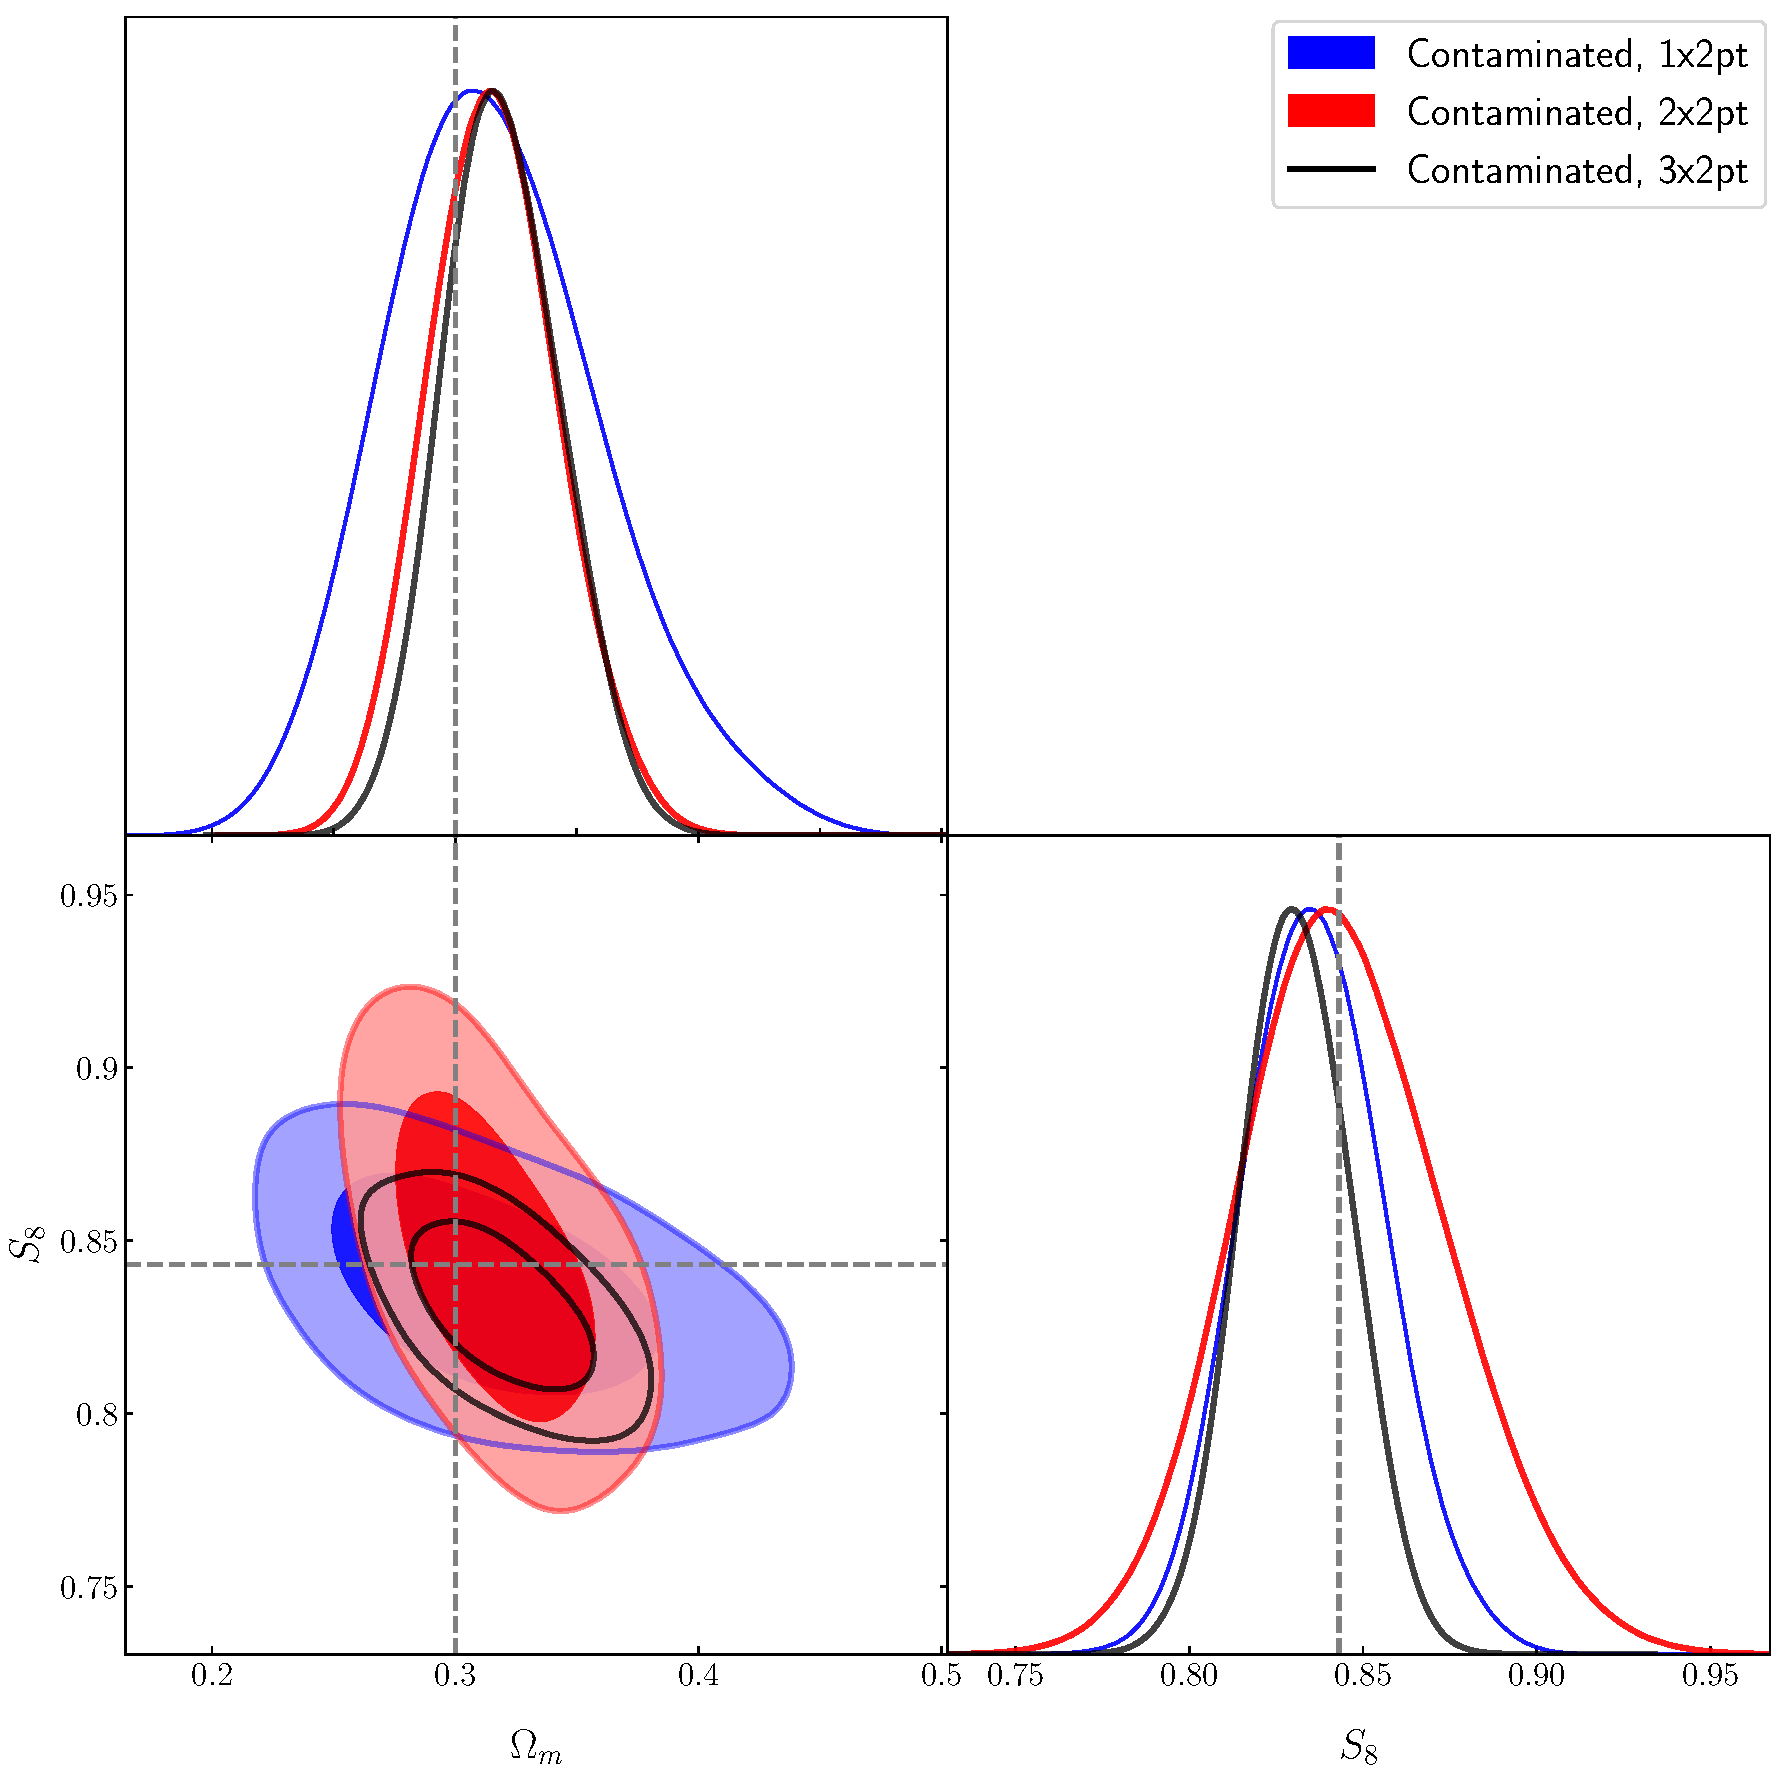
\includegraphics[width=\columnwidth]{figs/compare_all_cosmo_3x2pt_lcdm_contaminated.pdf}
\caption[]{SIMULATED: Compare the constraints from \textit{simulated} cosmic shear (1x2pt),  2x2pt and 3x2pt  with linear bias + halofit model with the same scale cuts (preferably fiducial 3x2pt cuts) for $\Lambda$CDM. This figure shows that 2x2pt adds complementary information to shear only constraints. Particularly, 2x2pt provides stronger constraints on $\Omega_m$. \red{Update this figure with current settings and with baseline DV.}}
\label{fig:all2pt_comp}
\end{figure}


\section{Statistics and theory}
\label{sec:stat_theory}
\subsection{Two-point statistics}
Using the catalog of the positions of foreground lens galaxies and the catalog of shape and positions of background source galaxies, one can construct three two point summary statistics. The two point auto-correlation of the positions of lens galaxies (galaxy clustering), auto-correlation of the lensing shear estimated from shape of background source galaxies (cosmic shear) and  cross-correlation of this lensing shear field and position of lens galaxies (galaxy-galaxy lensing). 

In this study we focus on galaxy clustering and galaxy lensing. For the galaxy clustering we use the $w(\theta)$ statistic which quantifies the average excess number of galaxy pairs at a separation $\theta$ over a random distribution. For galaxy-galaxy lensing, we use the statistic of $\gamma_{\rm t}(\theta)$ that describes the average excess tangential component of the shear at different lens-source separation. 

We use perturbation theory (PT) to make theoretical predictions for these two-point statistics as described below. 

\subsubsection{Power spectrum}
\label{sec:Pk_pred}

To compute the two-point porjected statistics $\wtheta$ and $\gammat$, we first describe our methodology of predicting galaxy-galaxy and galaxy-matter power spectrum ($\pgg$ and $\pgm$ respectively). PT is a powerful framework that describes the distribution of any biased tracer of underlying dark matter field in quasi-linear and linear scales. This framework allows for an order-by-order controlled expansion of the overdensity of biased tracer (here galaxies) in terms of overdensity of dark matter field where successively higher-order non-linearities dominate only in successively smaller scale modes. We will analyze two PT models in this analysis, an effective linear bias model (that is complete only up-to first order) and an effective 1Loop PT model (that is complete up-to third order). 

For the linear bias model, we can write the galaxy-matter cross spectrum as $P_{\mathrm{gm}}(k) = b_1 P_{\mathrm{mm}}$ and auto power spectrum of the galaxies as $P_{\mathrm{gg}}(k) = b_1^2 P_{\mathrm{mm}}(k)$. Here $b_1$ is the linear bias parameter and $P_{\mathrm{mm}}(k)$ is the non-linear auto power spectrum of the matter field. 

We use the non-linear matter power spectrum prediction from \citet{Takahashi:2012em} to model (\textsc{Halofit} hereafter) $P_{\mathrm{mm}}(k)$. We use \citet{Bird_halofit} prescription to model the impact of massive neutrinos in this \textsc{Halofit} fitting formula. See \red{Methods Paper} for robustness test of this choice.  

% \red{We use the halofit as our fiducial choice of matter power spectra. See Methods paper for robustness tests on this choice}
% We discuss our choice of matter power spectrum in \S\red{matter section}.

In the effective 1Loop PT model that we use, $P_{\mathrm{gm}}$ and $P_{\mathrm{gg}}$ can be expressed as:
\begin{align}\label{eq:P_gg_gm}
    P_{\mathrm{gm}}(k, z) &= b_1 P_{\mathrm{mm}}(k, z) +  \frac{1}{2} b_2 P_{\rm b_1 b_2}(k, z) + \frac{1}{2} b_{\mathrm{s}} P_{\rm b_1 s^2}(k, z) \nonumber  \\
    & + \frac{1}{2} b_{\rm 3nl}P_{\rm b_1 b_{\rm 3nl} }(k, z) \\
    P_{\mathrm{gg}}(k, z) &= b_1^2 P_{\mathrm{mm}}(k, z) + b_1 b_2 P_{\rm b_1 b_2}(k, z) + b_1 b_{\mathrm{s}}P_{\rm b_1 s^2}(k, z) \nonumber \\ 
    & + b_1b_{\rm 3nl} P_{\rm b_1 b_{\rm 3nl} }(k, z) + \frac{1}{4}b_2^2 P_{\rm b_2 b_2}(k, z) + \frac{1}{2} b_2 b_{\mathrm{s}}P_{\rm b_2 s^2}(k, z)  \nonumber \\ 
    & + \frac{1}{4} b^2_{\mathrm{s}} P_{\rm s^2 s^2}(k, z).  
\end{align}

Here the parameters $ b_1 $, $ b_2 $, $ b_{\mathrm{s}} $ and $ b_{\rm 3nl} $ are the renormalized bias parameters \citep{McDonald2009}. \red{Describe the kernels briefly as well.} In \cite{p2020perturbation} we analyzed this model using 3D correlation functions ($\xigg$ and $\xigm$, which are Fourier transform of power spectra mentioned above) of \redmagic galaxies measured in DES-like simulations. We found that this model provides a good description of the high signal-to-noise 3D measurements above scales of 4 Mpc/h and redshift $z < 1$. Our tests also showed that at the projected precision of this analysis, two of the nonlinear bias parameters ($ b_{\mathrm{s}} $ and $ b_{\rm 3nl} $) can be fixed to their co-evolution values. We will use this result as our \textit{fiducial} modeling choice of the 1Loop PT model. 

% \begin{itemize}
%     \item Heavily referencing the 3D bias paper, describe range of perturbation theory models for $\xigg(r)$ and $\xigm(r)$ and their expected scales of applicability. 
%     \item To aid discussion, include some plots showing the sensitivity of our statistics to scales in $\xigg(r)$ and $\xigm(r)$.
% \end{itemize}

\subsubsection{Projected statistics}
\label{sec:proj_2pt}
% \begin{itemize}
%     \item Describe the statistics we use, \wtheta\ and \gammat.
%     \item Show their relation to the underlying 3d correlation functions $\xigg(r)$ and $\xigm(r)$
% \end{itemize}

In order to calculate our observable $\wtheta$ and $\gammat$, we first project the 3D power spectra to angular coordinates. Assuming that the normalized redshift distribution of the galaxies is denoted by $n^{i}_g(z)$ and of source galaxies is denoted by $n_{\rm s}$, the projected galaxy clustering (AB = gg) and galaxy-galaxy lensing (AB=${\rm g\kappa}$, where $\kappa$ denotes the convergence field) angular power spectrum are given by:
\begin{align}\label{eq:Cl_exact}
    C^{ij}_{\rm AB}(\ell) &= \frac{2}{\pi} \int d\chi_1 W^{\rm i}_{\rm A}(\chi_1) \int d\chi_2 W^{\rm j}_{\rm B}(\chi_2) \nonumber \\
    &\mathrel{\phantom{=}} \int dk \ k^2 \ P_{\rm AB}(k,z(\chi_1),z(\chi_2)) j_{\ell}(k \chi_1) j_{\ell}(k \chi_2)
\end{align}
Here $W^{\rm i}_{\rm g} = n^{i}_g dz/d\chi$ is the normalized selection function of galaxies for tomographic bin $i$ and $W^{\rm i}_{\rm \kappa}$ is the tomographic lensing efficiecy given by:
\begin{equation}
    W^{\rm i}_{\rm \kappa} = \frac{3\Omega_m H_0^2}{2} \int_{\chi}^{\infty} d\chi' n'_{\rm s} \frac{\chi}{a(\chi)}\frac{\chi' - \chi}{\chi'}
\end{equation}


For the galaxy-galaxy lensing observable, we use Limber approximation which simplifies the above equation as follows:
\begin{equation}\label{eq:Cl_limber}
    C^{ij}_{\rm g\kappa}(\ell)  = \int d\chi \frac{W^{\rm i}_{\rm g}(\chi) W^{\rm i}_{\rm \kappa}(\chi)}{\chi^2} P_{\rm g\kappa}\bigg(k=\frac{l + 1/2}{\chi},z(\chi)\bigg) 
\end{equation}
In the absence of other modeling ingredients that are described in the next section, we have $C^{ij}_{\rm g\kappa}(\ell) = C^{ij}_{\rm gm}(\ell)$ (similarly $P_{\rm g\kappa} = P_{\rm gm}$). As described in \citet{Fang_nonlimber}, even at the accuracy beyond this analysis, it is sufficient to use Limber approximation for galaxy-galaxy lensing observable while for galaxy clustering, this may cause significant cosmological parameter biases. 

To model the non-limber correction for the galaxy clustering, we split the predictions into small and large scale parts. The non-limber correction is only significant on large scales where non-linear contributions to the matter power spectra as well as galaxy biasing are sub-dominant. Therefore we use Limber approximation for the small scale non-linear corrections and use non-limber corrections strictly on large scales using linear theory. In the absence of contributions from other physical processes, the galaxy clustering angular power spectrum between tomographic bins $i$ and $j$ is given by:
\begin{align}\label{eq:Clgg_exact}
    &C_{\rm gg}^{ij} (\ell) \nonumber\\
    &= \int d\chi\, \frac{W_{\rm g}^i(\chi)W_{\rm g}^j(\chi)}{\chi^2} \left[P_{\rm gg}\left(\frac{\ell+0.5}{\chi},\chi\right)- b_1^{i} b_1^{j} P_{\rm lin}\left(\frac{\ell+0.5}{\chi},\chi\right)\right]\nonumber\\
    &+\frac{2}{\pi}\int d\chi_1\,b_{1}^i W_{\rm g}^i(\chi_1) D(z(\chi_1))\int d\chi_2\,b_{1}^j W_{\rm g}^j(\chi_2)D(z(\chi_2))\nonumber\\
    &\;\;\;\;\times \int\frac{dk}{k}k^3 P_{\rm lin}(k,0)j_\ell(k\chi_1)j_\ell(k\chi_2)\,,
\label{eq:Cl-DD_rewrite}
\end{align}
where, $D(z(\chi)$ are the growth factors and $P_{\rm lin}$ is the linear matter power spectrum. The full model of galaxy clustering including the contributions from other modeling ingredients like redshift space distortions and lens magnification that we describe below is detailed in \cite{Fang_nonlimber} and \red{Methods Paper}. 

The real space projected statistics of our interest can be obtained from these angular correlation via:
\begin{align}\label{eq:2pt_exact}
    w^{ij}(\theta) &= \sum \frac{2\ell + 1}{4\pi} \overline{P_{\ell}}(\cos(\theta)) \ C^{ij}_{\rm gg}(\ell) \\
    \gamma_{\rm t}^{ij}(\theta) &= \sum \frac{2\ell + 1}{4\pi \ell (\ell + 1)} \overline{P_{\ell}^2}(\cos(\theta)) \ C^{ij}_{\rm g\kappa}(\ell)
\end{align}
where $\overline{P_{\ell}}$ and $\overline{P_{\ell}^2}$ are bin-averaged Legendre Polynomials (see \red{Cov-Paper} for exact expressions). 

\subsection{The rest of the model}
\label{sec:model_rest}
In order to describe the statistics measured from data, we have to model various other physical phenomena that contribute to the signal in order to obtain unbiased inferences. In this section we describe the leading sources of these modeling systematics. We have also validated in \red{Methods paper} that higher order corrections do not bias our results. 

\subsubsection{Intrinsic Alignment} 
Galaxy galaxy lensing aims to isolate the percent-level coherent shape distortions, or shear, of background source galaxies due to gravitational field of foreground lens galaxies. However, the local environment can align the source galaxies as well as also contribute to the shear signal through lensing distortions. Since this interaction between the source galaxies and their local environment is non-random, it has non-zero contribution to the galaxy-galaxy lensing signal which we describe using TATT (tidal alignment tidal torquing) model \citep{Blazek_2019}. To the first order, this contributes linearly to the galaxy-shear angular power spectra and hence we have $C^{ij}_{\rm g\kappa}(\ell) \to C^{ij}_{\rm g\kappa}(\ell) + C^{ij}_{\rm gI_{\rm E}}(\ell)$. The correlation between the intrinsic alignment E-mode and galaxy density field ($C^{ij}_{\rm gI_{\rm E}}(\ell)$) is detailed in \red{Methods paper}, \red{CosmicShear2} and \citet{Blazek_2019}. Within the TATT framework, $C^{ij}_{\rm gI_{\rm E}}(\ell)$ for all tomographic bin combinations $i$ and $j$ can be expressed using five constants, $A_1$, $A_2$, $\alpha_1$, $\alpha_2$ and $b_{\rm ta}$. \red{Mention that we ignore the coupling of non-linear galaxy-bias model and this non-linear IA model. Mention some references on why this will be a small effect and that we leave this for future work.}

\subsubsection{Magnification}
All the matter between observed galaxy and the observer acts as a gravitational lens. Hence the galaxies get magnified which results in an increase in the size of galaxy images (parameterized by magnification factor, $\mu$) as well as increase in their total flux. The increase in the size of galaxies results in decrease in observed number density (due to stretching of local sky), whereas due to increase in total flux results in increase in number density (as intrinsically fainter galaxies, which are more numerous, can be observed). This changes the galaxy-galaxy angular power spectrum to: $C^{ij}_{\rm gg}(\ell) \to C^{ij}_{\rm gg}(\ell) + C^{ij}_{\rm \mu g}(\ell) + C^{ij}_{\rm \mu \mu}(\ell) $ and the galaxy-shear angular power spectrum to $C^{ij}_{\rm g\kappa}(\ell) \to C^{ij}_{\rm g\kappa}(\ell) + C^{ij}_{\rm \mu I_{\rm E}}(\ell) + C^{ij}_{\rm \mu \kappa}(\ell)$. \red{The auto and cross-power spectra with magnification are again given by Eq.\ref{eq:Cl_exact}. See Methods paper for exact description of the equations for each of the power spectra. Show the snippet of Equation here and say that we fix the magnification coefficients as a fiducial run. Say that we show the free magnification run for the linear bias model in the Fig. X}. 
The magnification coefficients are computed with the Balrog image simulations \cite{Suchyta2016,balrog} in a process described in \cite{magnification}. 
%Galaxy profiles are drawn from the DES deep fields \cite{deepfields} and injected into real DES images. The full photometry pipeline \cite{Y3Gold} and \redmagic\ sample selection is applied to the new images to produced a simulated \redmagic\ sample with the same selection effects as the real data. To compute the impact of magnification, the process is repeated, this time applying a constant magnification to each injected galaxy. The magnification coefficients are then derived from the fractional increase in number density when magnification is applied. This method captures both the impact of magnification on the galaxy magnitudes and the galaxy sizes, including all numerous sample selection effects. 

\subsubsection{Redshift space distortions}    
The large scale veolcity flow distorts the distribution of the galaxies along the line of sight. To the first order this can be approximated with a linear Kaiser flow factor.  

\subsubsection{Non-locality of galaxy-galaxy lensing}  
\label{sec:pm_theory}
The configuration space estimate of galaxy-galaxy lensing signal is a non-local statistic even on linear scales. The galaxy-galaxy lensing signal of source galaxy at redshift ($z_{\rm s}$) by the matter around galaxy at redshift $z_{\rm l}$ at perpendicular to the line of sight distance $R$ is related to the mass density of matter around lens galaxy by:
\begin{equation}
    \gamma_{\rm t}(R;z_{\rm g},z_{\rm s}) = \frac{\Delta \Sigma (R;z_{\rm l})}{\Sigma_{\rm crit} (z_{\rm g},z_{\rm s})},
\end{equation}
where, $\Delta \Sigma(R;z_{\rm l}) = \bar{\Sigma}(0,R; z_{\rm l}) - \Sigma(R;z_{\rm l})$ and $\Sigma(R;z_{\rm l})$ is the surface mass density at a transverse separation $R$ from the lens and $\bar{\Sigma}(0,R)$ is the average surface mass density within a separation $R$ from that lens. Through $\bar{\Sigma}(0,R)$ term, $\gamma_{\rm t}$  at any scale $R$, is dependent on mass distribution at all scales less than $R$. This makes $\gamma_{\rm t}$ statistic highly non-local and any model that is valid only on large scales above some $r_{\rm min}$ (like PT) will break down more rapidly than for a more local statistic like \wtheta. However, as the dependence on small scales is through the \textit{mean} surface mass density, the impact of mass distribution inside $r_{\rm min}$ on \gammat can be written as:
\begin{equation}
    \gamma_{\rm t}(R;z_{\rm g},z_{\rm s}) = \frac{1}{\Sigma_{\rm crit}(z_{\rm g},z_{\rm s})} \bigg(\Delta \Sigma_{\rm model}(z_{\rm g}) + \frac{B(z_{\rm g})}{R^2} \bigg),
\end{equation}
where, $\Delta \Sigma^{\rm model}$ is the prediction from a model (which in here is given by PT) that is valid of scales above $r_{\rm min}$. Here, $B$ is the effective total residual mass below $r_{\rm min}$ and is known as point mass (PM) parameter. In this analysis we use the thin redshift bin approximation (\red{see Appendix X for details of this validation}) and hence the average $\gamma_{\rm t}$ signal between lens bin $i$ and source bin $j$ can be written as:
\begin{equation}
    \gamma^{ij}_{{\rm t}} = \gamma^{ij}_{{\rm t, model}} + C^{ij}/\theta^2,
\end{equation}
where,

\begin{equation}\label{eq:pm_Cij}
    C^{ij} = B^i \, \int dz_{\rm g} \ dz_{\rm s} \ n^{i}_{{\rm g}} \ n^{j}_{{\rm s}} \ \Sigma^{-1}_{\rm crit}(z_{\rm g},z_{\rm s}) \ \chi^{-2}(z_{\rm g}) \equiv B^i \, \beta^{ij}
\end{equation}
Here $B^i$ is the PM for lens bin $i$, $n^{i}_{{\rm g}}$ is the redshift distribution of lens galaxies for tomographic bin $i$, $n^{j}_{{\rm s}}$ is the redshift distribution of source galaxies for tomographic bin $j$. Note that this approximation also retains the shear ratio information in our analysis. 

However, instead of directly sampling over the parameters $B^i$ for each tomographic bin, we implement an analytic marginalization scheme as described in \red{PM-paper}. We modify our inverse covariance when calculating the likelihood as described in \S\ref{sec:cov_pm}

% \red{Describe how in current implementation the PM retains the shear-ratio} information


    % \begin{itemize}
    % \item Point-mass marginalization 
    % \item  Motivate that we will be using the $\Sigma^{-1}_{\rm crit}$ factors when doing the PM marginalization. 
    % \item \textbf{\textit{Figure}} Plot comparing the contours with vs without PM marginalization for both 2x2pt and 3x2pt. Make (or show) the argument that it is because of breaking of degeneracy between PM and S8. Basically make the case that PM does not matter for 3x2pt and that 2x2pt can have more aggressive scale cuts than 3x2pt analysis.
    % \end{itemize}
    
    
        
    
    
% \subsubsection{PM Methods}
% The galaxy-galaxy lensing signal in configuration space is a non-local quantity and is sensitive to the galaxy-matter correlations in small scales. Therefore our perturbative theory model, which breaks down below some quasi-linear scales ($r_{\rm min}$), will result in a biased estimate of galaxy-galaxy lensing signal, even on large scales. However, all the non-local contribution to the galaxy-galaxy lensing signal at an angular separation theta from small scales can be parameterized with:
% \begin{equation}
%     \gamma^{ij}_{{\rm t}} = \gamma^{ij}_{{\rm t}, {\rm model}} + C^{ij}/\theta^2,
% \end{equation}
% where for tomographic bins $i$ and $j$, $\gamma^{ij}_{{\rm t}, {\rm model}}$ is our perturbation theory estimate of the galaxy-galaxy lensing signal and,
% \begin{equation}\label{eq:pm_Cij}
%     C^{ij} = B^{i} \bigg( \int dz_{\rm l} \ dz_{\rm s} \ n^{i}_{{\rm l}} \ n^{j}_{{\rm s}} \ \Sigma^{-1}_{\rm crit}(z_{\rm l},z_{\rm s}) \ \chi^{-2}(z_{\rm l}) \bigg).
% \end{equation}

% Here $B^{i}$ are the free parameters that are proportional to the average difference in the predicted and true enclosed mass below $r_{\rm min}$ surrounding the lens galaxies. However, instead of sampling the unknown constant $B^{i}$ parameters, we perform an analytic marginalization by modifying the covariance matrix. As described in \citet{MacCrann19}, this procedure can be performed by modifying the $\gamma_{{\rm t}}$ block of the inverse covariance matrix as follows:



% \begin{itemize}
    
    
%     \item projection of $P(k)$s to $C_l$ and conversion of $C_l$s to $w(\theta),\gamma_t(\theta)$.
% \end{itemize}

% \begin{figure}
% \includegraphics[width=\columnwidth]{figs/pm_evolution.png}
% \caption[]{ Evolution galaxy correlation function across the first redshift bin and its contribution to PM till 6Mpc/$h$.  }
% \label{fig:pm_evolve}
% \end{figure}
 

\section{Data description}

\subsection{DES Y3}

The full DES survey was completed in 2019 and cov- ered ∼ 5000 square degrees of the South Galactic Cap. Mounted on the Cerro Tololo Inter-American Observa- tory (CTIO) 4 m Blanco telescope in Chile, the 570- megapixel Dark Energy Camera [DECam 42] images the field in grizY filters. The raw images are processed by the DES Data Management (DESDM) team [43, 44]. The Year 3 (Y3) catalogs of interest for this study span the full footprint of the survey but with fewer exposures than the complete survey. About 100 million galaxies have shear and photometric redshift measurements that enable their use for cosmology. For the full details of the data and the galaxy and lensing shear catalogs, we refer the readers to [45] and [46].


\red{Describe DES and its dataproducts}
\subsubsection{Lens $\redmagic$ galaxy sample}

The lens sample used in this analysis is selected with the \redmagic algorithm run on DES Year 3 data. \redmagic selects Luminous Red Galaxies (LRGs) according to the magnitude-color-redshift relation of red sequence galaxies, calibrated using an overlapping spectroscopic sample from \red{<SPEC Z SAMPLE, OZDES? ask Eli>}. This sample has a threshold luminosity $L_{\rm min}$ and constant co-moving density. The full \redmagic algorithm is described in \cite[redmagicSV].



In \cite{clustering} it was found the \redmagic number density fluctuates with a number of observational properties of the survey. This imprints a non-cosmological bias into the galaxy clustering. To account for this we assign a weight to each galaxy which corresponds to the inverse of the angular selection function at that galaxies location. The computation and validation of these weights is described in \cite{clustering}.  

\subsubsection{Source galaxy shape catalog}
\red{Describe the source galaxy selection and metacalibration shape estimate. Also describe the calibration of shear with image sims. Introduce the multiplicative shear bias parameter (?) or whatever strategy is finalized. }

% \subsubsection{Photoz calibration}

\subsection{Simulations}

\subsubsection{$\buzzard$ sims}
The \buzzard\ simulations are $N$-body lightcone simulations that have been populated with galaxies using the \textsc{Addgals} algorithm, endowing each galaxy with positions, velocities, spectral energy distributions, broad band photometry, half-light radii and ellipticities. Each pair of 2 Y3 simulations are produced from a set of 3 independent $N$-body lightcones with box sizes of $1.05,\, 2.6 \textrm{ and } 4.0\, (h^{-3}\, \rm Gpc^3)$, mass resolutions of $3.3\times10^{10},\, 1.6\times10^{11},\, 5.9\times10^{11}\, h^{-1}M_{\odot}$, spanning redshift ranges $0.0< z \leq 0.32$, $0.32< z \leq 0.84$ and $0.84< z \leq 2.35$ respectively. Together these produce $10,000$ square degrees of unique lightcone. The lightcones are run with the \textsc{L-Gadget2} $N$-body code, a memory optimized version of \textsc{Gadget2} \citet{Springel2005}, with initial conditions generated using \textsc{2LPTIC} at $z=50$ \citep{Crocce2012}. 

The \textsc{Addgals} model uses the relationship, $P(\delta_{R}|M_r)$, between a local density proxy, $\delta_{R}$, and absolute magnitude $M_r$ measured from a high resolution sub--halo abundance matching (SHAM) model in order to populate galaxies into these lightcone simulations. This model reproduces the absolute--magnitude--dependent clustering of the SHAM. Additionally, we employ a conditional abundance matching (CAM) model, assigning redder SEDs to galaxies that are closer to massive dark matter halo, in a manner that allows us to reproduce the color dependent clustering measured in the Sloan Digital Sky Survey Main Galaxy Sample (SDSS MGS) \cite{Addgals, DeRose2020b}. 

These simulations are ray-traced using the spherical-harmonic transform (SHT) configuration of \textsc{Calclens}, where the SHTs are performed on an $N_{\rm side}=8192$ \textsc{HealPix} grid \citep{Becker2013}. The lensing distortion tensor is computed at each galaxy position and is used to deflect the galaxy angular positions, shear galaxy intrinsic ellipticities, including effects of reduced shear, and magnify galaxy shapes and photometry. We have conducted convergence tests of this algorithm and found that resolution effects are negligible on the scales used for this analysis \cite{DeRose2019}.

Once the simulations have been ray-traced, we apply DES Y3 specific masking and photometric errors. In order to mask the simulations, we employ the Y3 footprint mask, but do not apply the bad region mask \citep{y3gold}, resulting in a footprint with an area of \jdr{XXX} square degrees. Each set of 3 $N$-body simulations yields 2 Y3 footprints, that contain \jdr{XXX} sq. degrees of overlap.

We apply a photometric error model to the simulate wide field photometric errors in our simulations. In order to select a lens galaxy sample, we run the \redmagic\ galaxy selection on our simulations using the same configuration as used in the Y3 data as described in \citet{y3lens}. A weak lensing source selection is applied to the simulations using psf-convolved sizes and $i$-band SNR in order to match the non-tomographic source number density, \jdr{XXX} $arcmin^{-2}$, in the \metacal\ source catalog. We employ the SOMPZ redshift estimation framework to our simulations in order to place galaxies into four source redshift bins with number densities of \jdr{XXX}. Once binned, we match the shape noise of the simulations to that measured in the \metacal\ catalog per tomographic bin, yielding shape noise values of \jdr{XXX}.

Two point functions are measured in the \buzzard\ simulations using the same pipeline as that used for the DES Y3 data, where we set \metacal\ responses and inverse variance weights equal to 1 for all galaxies, as these are not assigned in our simulation framework. Lens galaxy weights are produced in a manner similar to that done in the data, and applied in order to measure our clustering and lensing signals. \jwd{The clustering and galaxy-galaxy lensing predictions match the DES measurements to XXX accuracy}.

\subsubsection{$\mice$ sims}

\subsection{Datavector}

\subsubsection{Lens redshift methodology}
We split the \redmagic sample into 5 tomographic bins, selected on the \redmagic redshift point estimate quantity ZREDMAGIC. The bin edges used are $z=0.15, 0.35, 0.50, 0.65, 0.80, 0.90$. The first three bins use a luminosity threshold of $L_{\min} > 0.5 L_{*}$ and are known as the high density sample. The last two redshift bins use a luminosity threshold of $L_{\min} > 1.0 L_{*}$ and are known as the high luminosity sample.

The redshift distributions are computed by stacking 4 samples from the PDF of each individual \redmagic galaxy, allowing for the non-gaussianity of the PDF. From the variance of these samples we find an average individual redshift uncertainty of $\sigma_z/(1+z) < $ \red{NUMBER} in the redshift ranged used.

\subsubsection{Source redshift methodology}
\red{Describe the redshift binning of source sample. Describe SOMPZ as well as how clustering-z and shear ratios help with these redshift samples.}

The n(z)'s of lenses and sources are compared in the Fig.~\ref{fig:nz_comp}.


\subsubsection{2pt measurements}
\red{Describe the 2pt measurements for both $\wtheta$ and $\gammat$. Mention the combined SNR of these measurements. Mention that we do the measurements in the 20 radial bins for any two tomographic bin combinations. Mention that for $\wtheta$ we only use auto-bins. Introduce $N_{\rm data}$ and how it relates to the number of elements for $\wtheta$ and number of $\gammat$ elements.} 

\subsubsection{Blinding}

\subsubsection{Unblinding}


\subsection{Covariance}
We use a halo model framework to model the multiprobe covariance used in this analysis. The exact model and its robustness tests have been detailed in \red{Cov-Paper}. 

% Describe the fiducial covariance and the modifications due to point mass addition. 



\subsubsection{Point mass analytic marginalization}
\label{sec:cov_pm}

\begin{equation}
    {\mathbfcal{C}}^{-1}_{\rm wPM} = {\mathbfcal{C}}^{-1} - {\mathbfcal{C}}^{-1} {\mathbfcal{U}} ({\mathbfcal{I}} + {\mathbfcal{U}}^{\rm T} {\mathbfcal{C}}^{-1} {\mathbfcal{U}})^{-1} {\mathbfcal{U}}^{\rm T} {\mathbfcal{C}}^{-1}
\end{equation}

Here ${\mathbfcal{C}}^{-1}$ is the inverse of the halo-model covariance as described above and $\mathbfcal{U}$ is a $N_{\rm data} \times n_{\rm lens}$ matrix whole $i$-th column is given by $\sigma_{B^i} \vec{t}^{i}$. 

\begin{equation}
    \bigg(\vec{t}^{i} \bigg)_{a} = \begin{cases}
0 & \parbox{5cm}{if $a$-th element is not corresponding to $\gammat$ and if lens-redshift of $a$-th element $\neq i$} \\  
\beta^{ij}\theta_{a}^{-2} &\text{otherwise}
\end{cases}
\end{equation}
In our analysis we put a wide prior on PM parameters $B^i$ by choosing $\sigma_{B^i} = 10000$ which translates to effective mass residual prior of $10^{17} M_{\odot}/h$. 


\begin{figure}
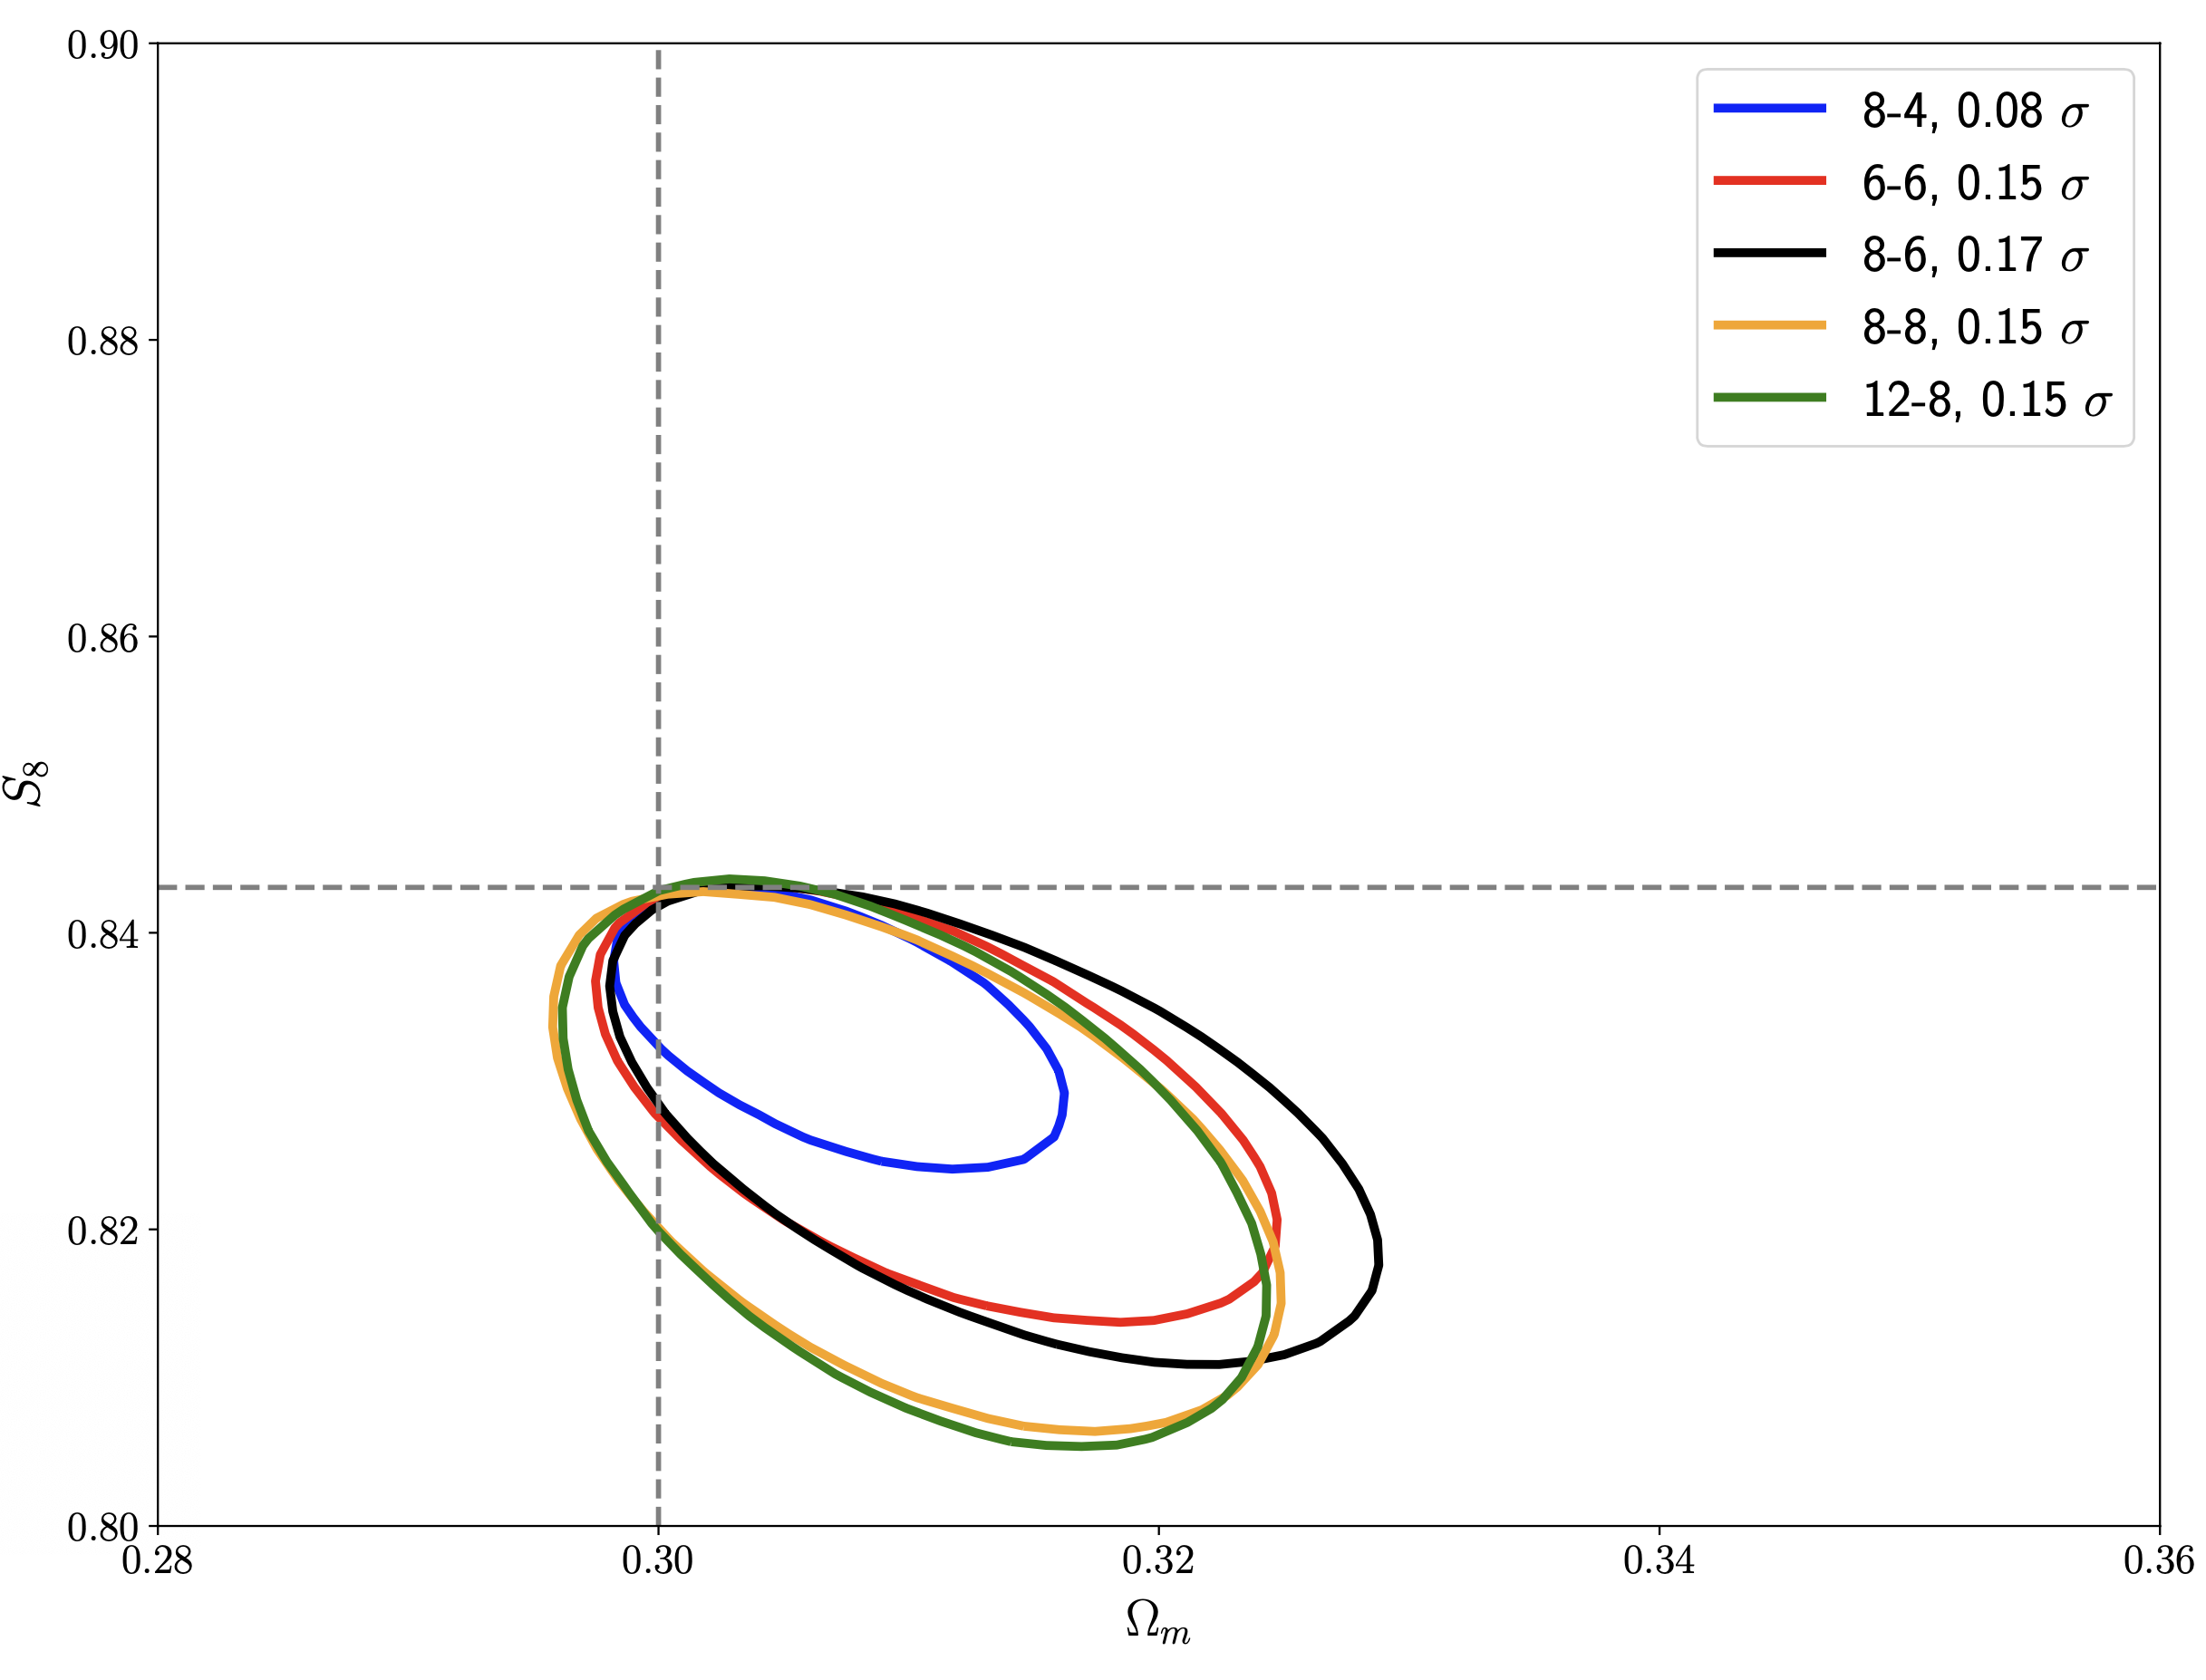
\includegraphics[width=0.5\textwidth,draft]{figs/temp.png}
\caption[]{Comparison of n(z)'s of sources and lenses in the data and in the \buzzard/\mice simulation. }
\label{fig:nz_comp}
\end{figure}

The datavectors, along with the best-fit theory models, for both the simulations and DES data are shown in the Appendix~\ref{app:2x2pt_measure}. 


\section{Validation of parameter inference}

We assume that the likelihood is a multivariate guassian and given as follows:
\begin{equation}
    \ln \mathcal{L}(\Theta) = -\frac{1}{2} (\vec{\mathbfcal{D}} - \vec{\mathbfcal{T}}(\Theta)) \, {\mathbfcal{C}}^{-1}_{\rm wPM} \,  (\vec{\mathbfcal{D}} - \vec{\mathbfcal{T}}(\Theta))^{\rm T}
\end{equation}

Here $\vec{\mathbfcal{D}}$ is the measured $\gammat$ and $\wtheta$ datavector of length $N_{\rm data}$, $\vec{\mathbfcal{T}}$ is the theoretical prediction for these statistics at some parameter point $\Theta$ and ${\mathbfcal{C}}^{-1}_{\rm wPM}$ is the inverse covariance matrix of shape $N_{\rm data} \times N_{\rm data}$, after including modifications from the PM marginalization term.

For our analysis we use \textsc{Polychord} sampler with the settings described in \red{Sampler paper}. 

% \red{Describe how the log-likelihood is calculated. Connect it with the inverse covariance described in the above section.}
% \red{Mention which sampler we are using, point to the appropriate settings?. Also probably to code comparison plots in the Methods paper}
\red{Which parameter statistic we quote. Describe why we choose mean of the marginalized posteriors. Also allude to the projection effects here. Mention that they are worse for the non-linear bias model and mention that we will discuss this further in later section }


\subsection{Analysis choices}
In this subsection we detail the galaxy biasing models that we use, description of the free parameters of our model and choice of priors on those parameters. 
\subsubsection{PT Models}
\label{sec:2x2pt_models}
We test two different galaxy bias models:
\begin{enumerate}
    \item \textit{Linear Bias} Model: Linear bias: As described in \S~\ref{sec:Pk_pred}, simplest model to describe the overdensity of galaxies is to assume it to be linearly biased with respect to the overdensity of dark matter. For each lens tomographic bin, the average bias of galaxies is given by a constant free parameter $b_1$. We use a wide uniform prior on the parameter for each lens tomographic bin $j$, given by $0.5 < b^{j}_1 < 3$. 
    \item \textit{Non-linear bias} Model: 
    In order to describe the clustering of galaxies in small scales robustly we also implement a 1Loop PT model. As described in the \S~\ref{sec:Pk_pred}
    , in general this model has four free bias parameters for each lens tomographic bin. We fix the parameters $b_{\rm s}$ and $b_{\rm 3nl}$ to their co-evolution values. In this model, for each tomographic bin, we have two free parameters, linear bias $b^{j}_1$ and non-linear bias $b^{j}_2$. \red{In the end we care about the posterior on the cosmology parameters. This requires marginalizing over all the free parameters of the model. $\wtheta$ and $\gammat$ has lower signal to noise and hence can not constrain the higher order parameters like $b^j_2$ tighthly. When projecting this to lower dimension space, the posterior-mass due to non-linear parameters being far from the truth can bias the constraints on the marginalized parameters due to subtle degeneracies. This is known as projection effect or volume effect.} We find that using a uniform prior on the linear and non-linear bias parameters leads to large projection effects.  Therefore, we choose to sample the parameters $b^{j}_1 \sigma_8$ and $b^{j}_2 \sigma^2_8$ which helps in removing much of the projection effect. \red{This choice is motivated because the overdensity of galaxy is approximately given by $\delta_g \sim b_1 \delta_m + b_2 \delta_m^2$.} We use wide uninformative uniform priors on these parameters for each tomographic bin $j$ given by : $0.67 < b^{j}_1 \sigma_8 < 3.0$ and $-4.2 < b^{j}_2 \sigma^2_8 < 4.2$. At each point in the parameter space, we calculate the $\sigma_8$ and retrieve the bias parameters $b^{j}_1$ and $b^{j}_2$ from the sampled parameters $b^{j}_1$ and $b^{j}_2$.
\end{enumerate}


\subsubsection{Cosmological Models}

% \subsection{Cosmological models, external datasets and priors}
We test the following cosmological model and prior combinations




We report the constraints on three choices of the cosmological model:
\begin{enumerate}
    \item Flat \lcdm\ with uninformative priors: We free five cosmological parameters $\Omega_m$, $\Omega_b$, $n_s$, $h_0$ and $A_s$ \red{$\Omega_\nu h^2$ ?}
    % \item Flat \lcdm\ with informative priors on some combination of $\Omega_m$, $H_0$ and $n_s$ TBD.
    \item Flat \wcdm : In addition to above mentioned five parameters, we also free $w_0$.
    \item Flat \wcdm\ with Planck : \red{Describe how we simulate Planck likelihood }
\end{enumerate}

\red{Mention that we will compare our constraints with a variety of external datasets as well that we can not simulate.}

\subsubsection{Scale cuts}

% \begin{figure}
% 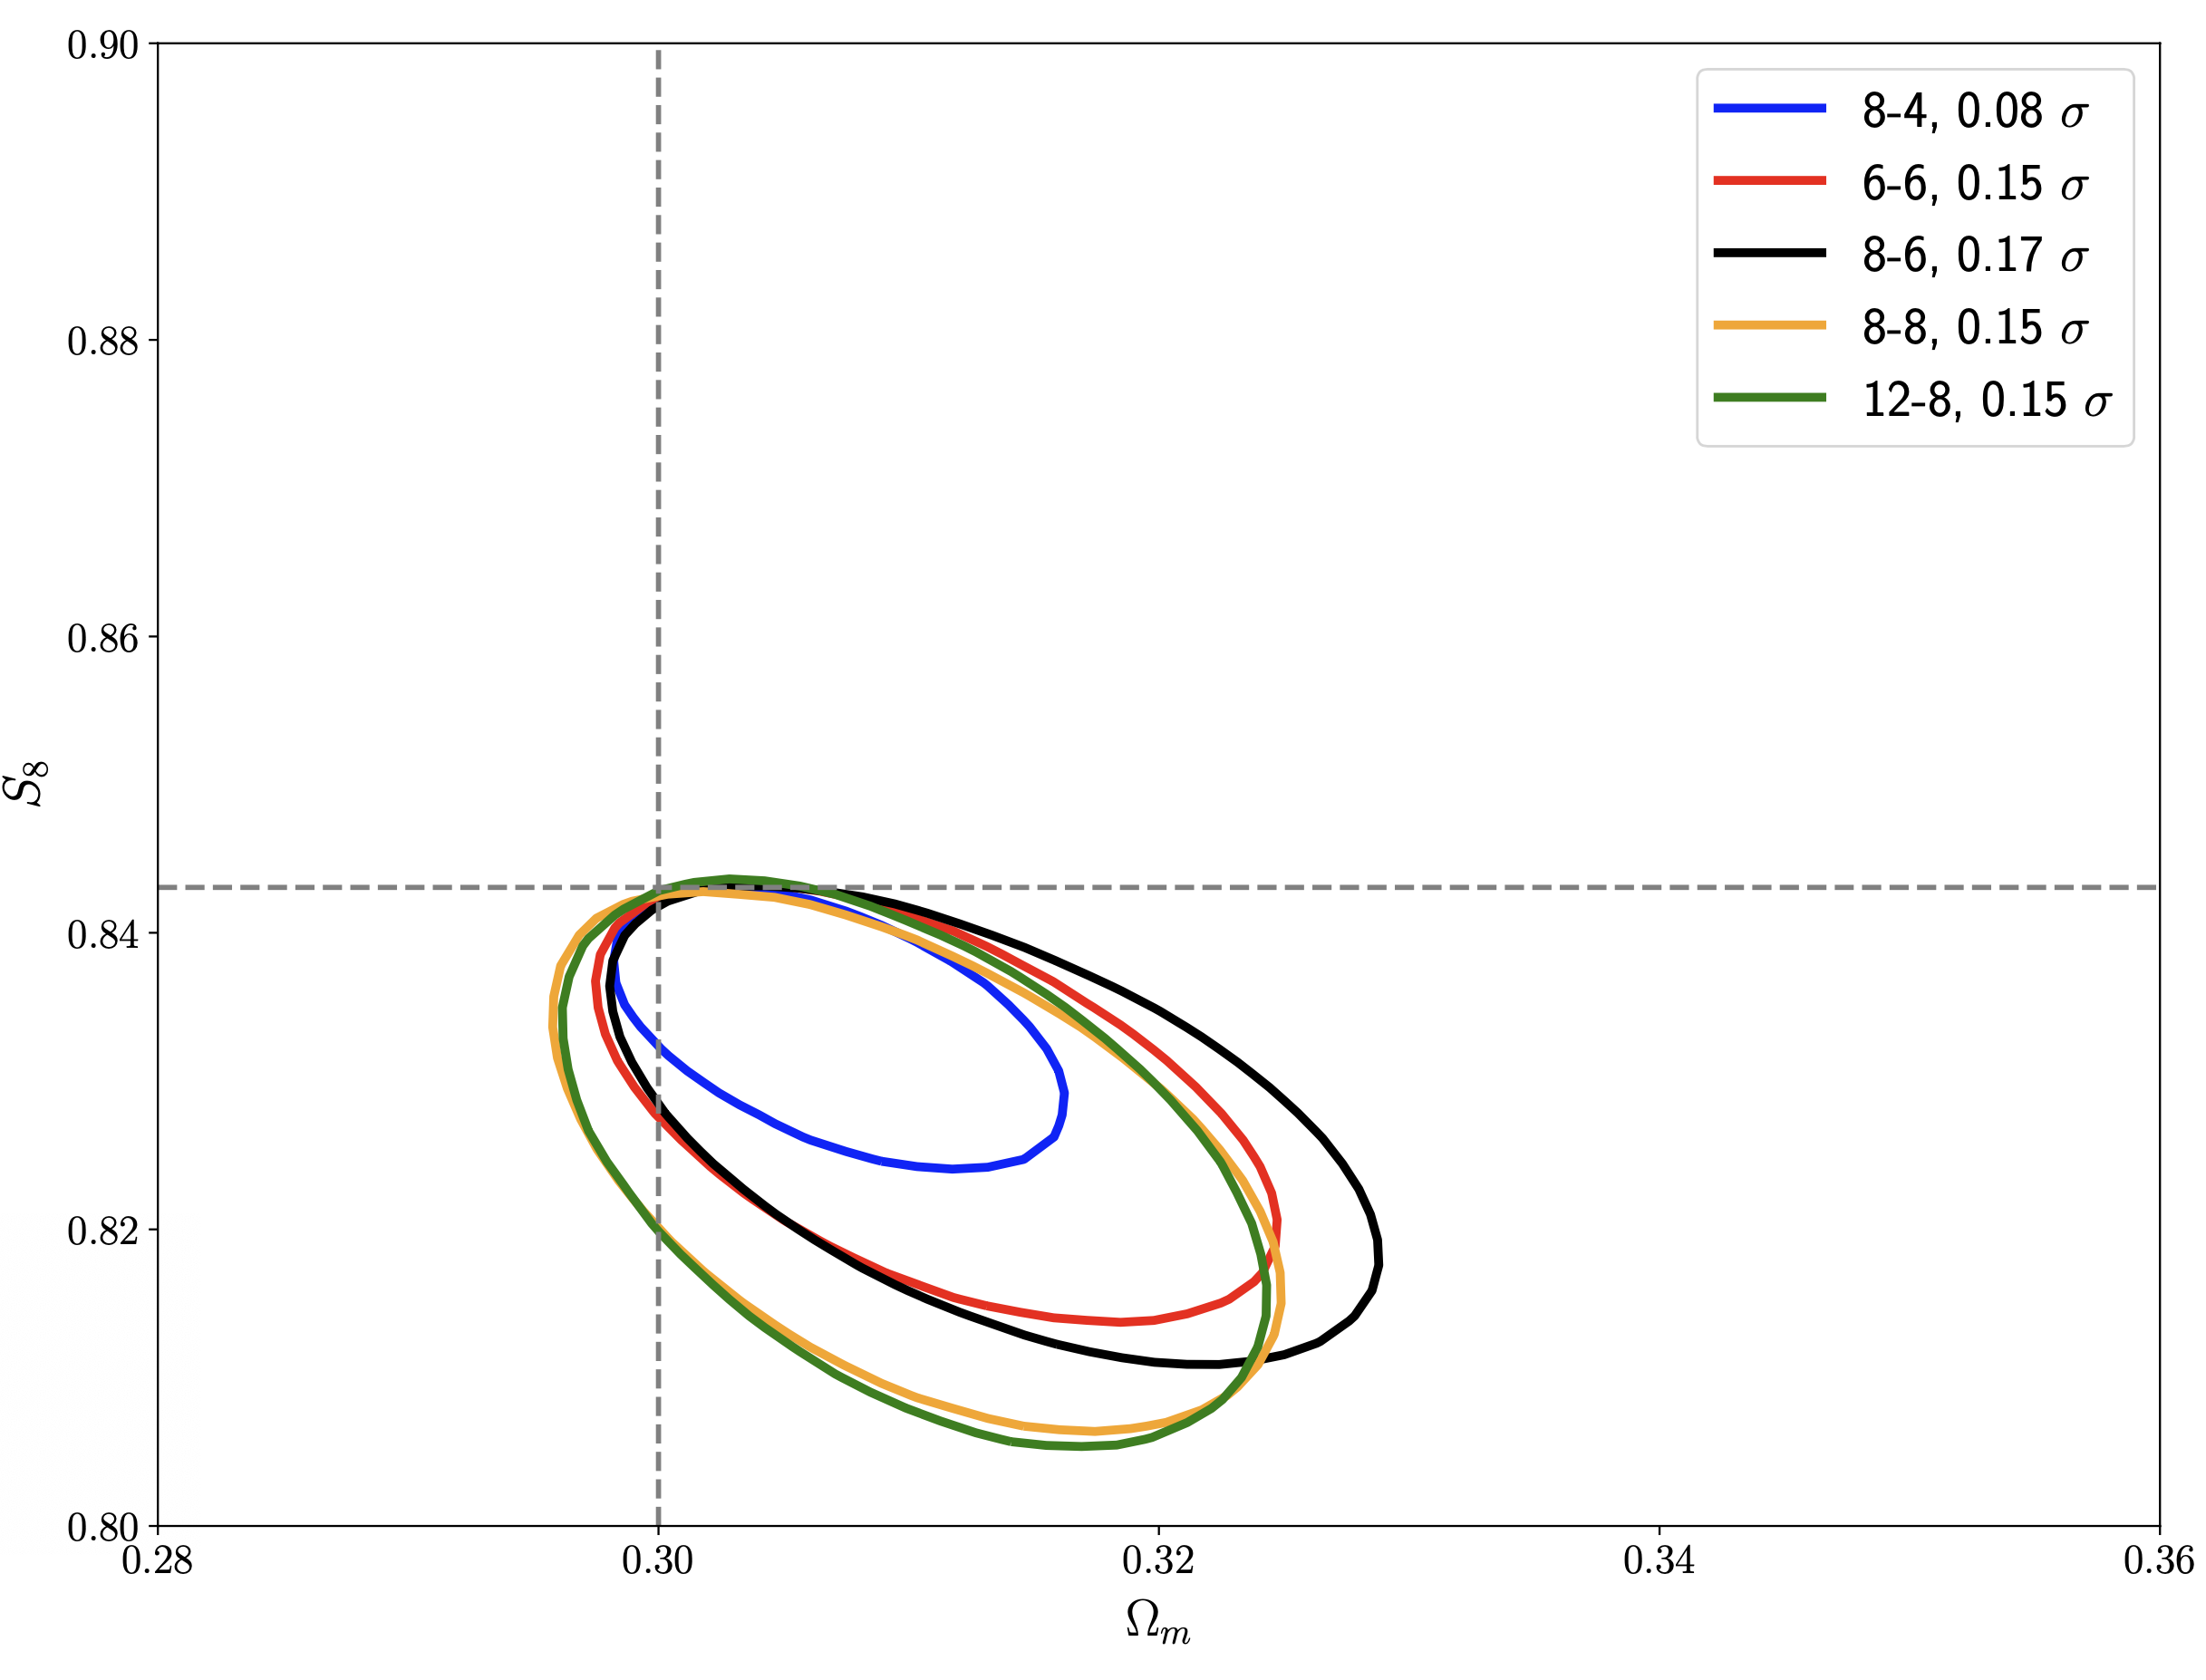
\includegraphics[width=0.5\textwidth,draft]{figs/temp.png}
% \caption[]{Show which radial scales contribute to each $\theta$ bin. This will connect to the 3D bias paper}
% \label{fig:scale_comp}
% \end{figure}



\red{Motivated by the 3D bias modelling paper, we choose 2 or 3 sets of scale cuts. Connect this to a figure showing how does different angular scales are impacted by the real space 3D correlation functions.}

From the tests on 3D correlation functions at fixed cosmology in simulations, we find that the linear bias approximation (Model A) is a good description above 8Mpc/$h$ while the two parameter non-linear bias model (Model B) can describe the correlations above 4Mpc/$h$. Starting with the scale cuts motivated from above study, we test various choices around it and quantify the biases we see in the recovered cosmological parameters.

\red{Mention the criteria for the scale cuts. Mention again the projection effects and why we choose to define this criteria in 2D plane of $\Omega_m$ - $S_8$. Moreover we run two set of chains, a baseline chain and a contaminated chain to capture the projection effects. And then we determine the minimum scales where the bias between the marginalized contours of the baseline and the contaminated contours in less than $0.3\sigma$. Also mention that we do this exercise for both $\Lambda$CDM and $w$CDM cosmology. In case of $w$CDM, we look at all three 2D combinations constructed out of $\Omega_m$, $S_8$ and $w$.}



\subsubsection{Priors}
\red{Motivate the choice of the priors and make a distinction between the informative and non-informative priors on different parameters. }
% \begin{figure}
% 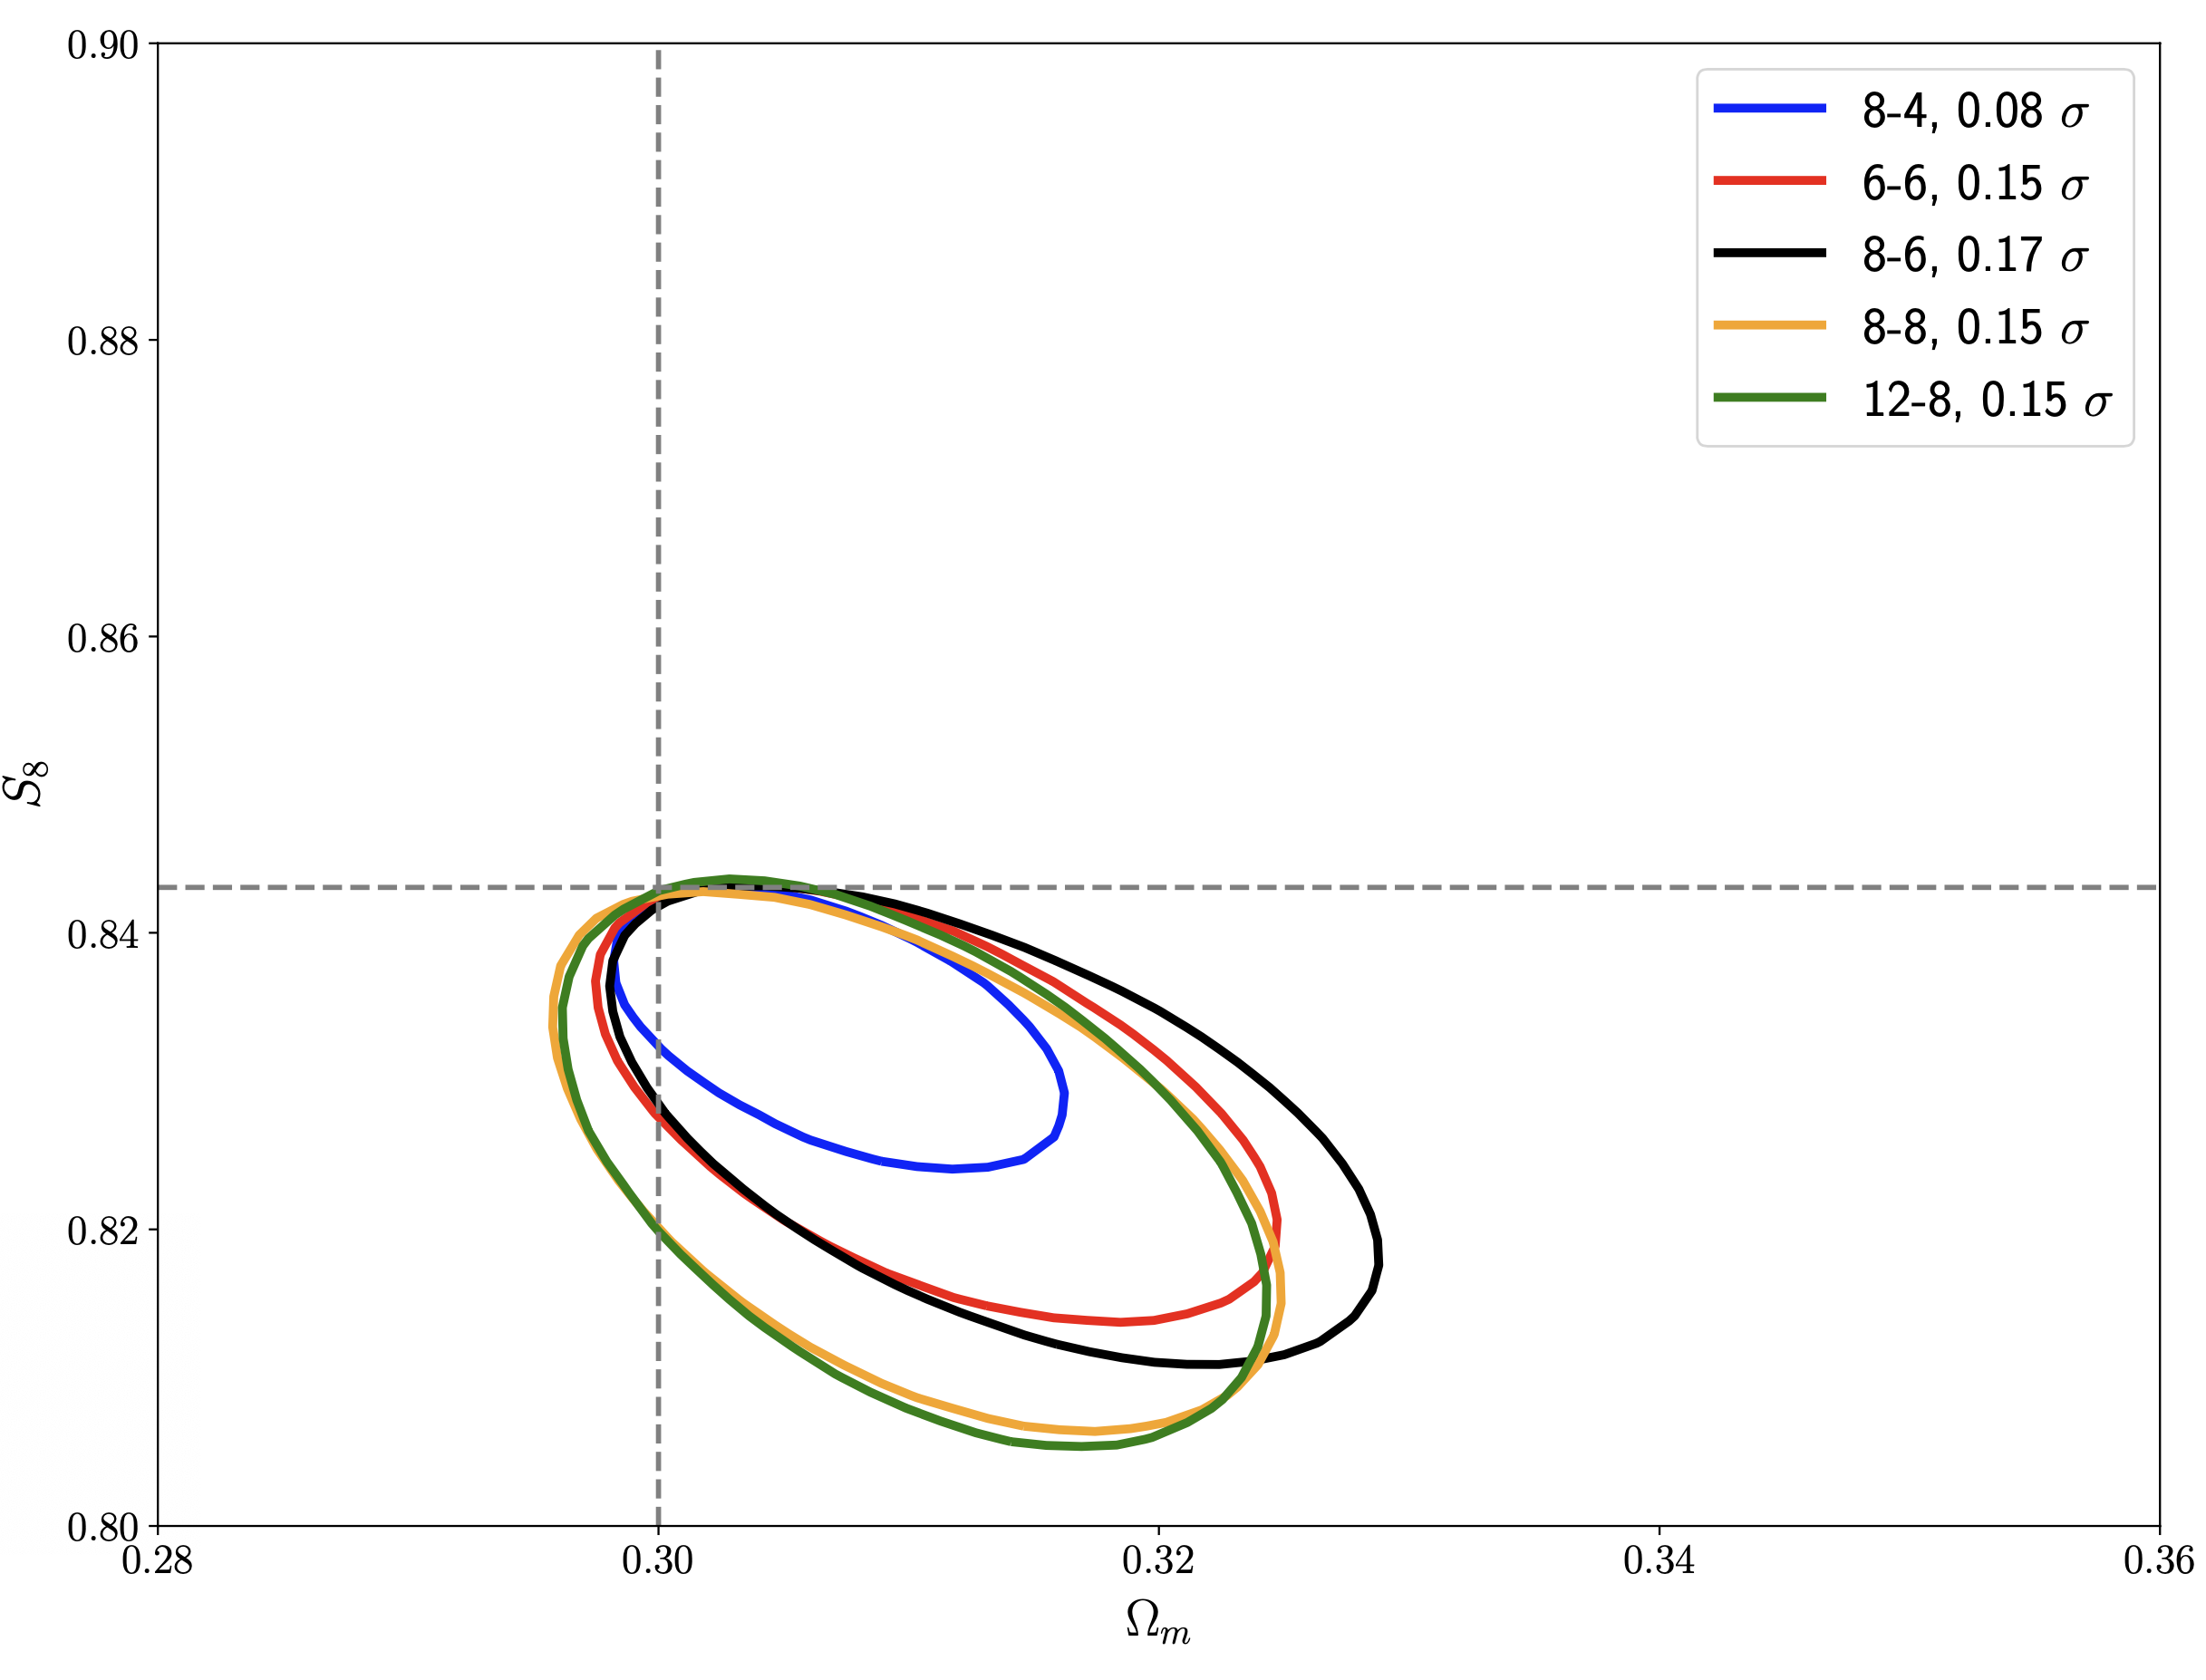
\includegraphics[width=0.5\textwidth,draft]{figs/temp.png}
% \caption[]{Put a table describing all the parameters that we vary and the priors that we put for both \textit{Liner bias} and \textit{Non-linear Bias} model.  }
% \label{fig:table}
% \end{figure}

% \begin{table}
% \begin{tabular}{|l| l l l|}
% \hline
% % \hline
% Model & Parameter & Prior & Posterior  \\ \hline
% & \multicolumn{3}{c|}{Cosmology} \\ 
% \multirow{4}{*}{Common} & $\Omega_m$ & $\mathcal{U}[0.1, 0.9]$ & $0.3^{+0.1}_{-0.1}$ \\
%  & $A_s$ & $\mathcal{U}[5\times 10^{-10}, 5\times 10^{-9}]$ & $1\times 10^{-9}^{+1\times 10^{-9}}_{-1\times 10^{-9}}$ \\
 
% & $\Omega_b$ & $\mathcal{U}[0.03, 0.07]$ & $0.044^{+0.01}_{-0.01}$ \\

% & $n_s$ & $\mathcal{U}[0.87, 1.06]$ & $0.9^{+0.1}_{-0.1}$ \\

% & $h$ & $\mathcal{U}[0.87, 1.06]$ & $0.9^{+0.1}_{-0.1}$ \\

% & $\Omega_{\nu}h^2$ & $\mathcal{U}[0.87, 1.06]$ & $0.9^{+0.1}_{-0.1}$ \\ \\

% & \multicolumn{3}{c|}{Intrinsic Alignment} \\  
% & $A_1$ & $\mathcal{U}[0.87, 1.06]$ & $0.9^{+0.1}_{-0.1}$ \\
% & $A_2$ & $\mathcal{U}[0.87, 1.06]$ & $0.9^{+0.1}_{-0.1}$ \\
% & $\alpha_1$ & $\mathcal{U}[0.87, 1.06]$ & $0.9^{+0.1}_{-0.1}$ \\
% & $\alpha_2$ & $\mathcal{U}[0.87, 1.06]$ & $0.9^{+0.1}_{-0.1}$ \\
% & $b_{\rm ta}$ & $\mathcal{U}[0.87, 1.06]$ & $0.9^{+0.1}_{-0.1}$ \\


% & \multicolumn{3}{c|}{Lens photo-$z$} \\  
% & $\Delta z^{i}, i \in [1,5]$ & $\mathcal{G}[0.0, 0.004]$ & $0.9^{+0.1}_{-0.1}$ \\
% & \multicolumn{3}{c|}{Cosmology} \\ 
% \multirow{1}{*}{$w$CDM} & $w$ & $\mathcal{U}[-2, -0.33]$ & $-1^{+0.1}_{-0.1}$ \\ \hline

% \multirow{3}{*}{Midfielders} & MC & David Batty \\
%  & MC & Eirik Bakke \\
%  & MC & Jody Morris \\ \hline
% Forward & FW & Jamie McMaster \\ \hline
% \multirow{2}{*}{Strikers} & ST & Alan Smith \\
%  & ST & Mark Viduka \\
% \hline
% \end{tabular}
% \end{table}



% \begin{table}
% \begin{tabular}{|c| c c c|}
% \hline
% % \hline
% Model & Parameter & Prior & Remarks  \\ \hline
% % & \multicolumn{3}{c|}{Cosmology} \\ 
% % & & & \\
% & & & \\
% \multirow{24}{*}{\shortstack[c]{Common\\ Parameters}} & $\Omega_m$ & $\mathcal{U}[0.1, 0.9]$ & \multirow{6}{*}{\shortstack[c]{Cosmological\\ Parameters}} \\
%  & $A_s$ & $\mathcal{U}[5\times 10^{-10}, 5\times 10^{-9}]$ & \\
 
% & $\Omega_b$ & $\mathcal{U}[0.03, 0.07]$ &  \\

% & $n_s$ & $\mathcal{U}[0.87, 1.06]$ & \\

% & $h$ & $\mathcal{U}[0.87, 1.06]$ &  \\

% & $\Omega_{\nu}h^2$ & $\mathcal{U}[0.87, 1.06]$ & \\  
% & & & \\
% \cline{2-4}

% % & \multicolumn{3}{c|}{Intrinsic Alignment} \\ 
% & & & \\
% & $A_1$ & $\mathcal{U}[-5.0, 5.0]$ &\multirow{5}{*}{\shortstack[c]{Intrinsic\\ Alignment}} \\
% & $A_2$ & $\mathcal{U}[-5.0, 5.0]$ & \\
% & $\alpha_1$ & $\mathcal{U}[-5.0, 5.0]$ & \\
% & $\alpha_2$ & $\mathcal{U}[-5.0, 5.0]$ & \\
% & $b_{\rm ta}$ & $\mathcal{U}[0.0, 2.0]$ & \\ 
% & & & \\
% \cline{2-4}

% % & \multicolumn{1}{c|}{Lens photo-$z$} \\  
% & & & \\
% & $\Delta z^{1}$ & $\mathcal{G}[0.0, 0.004]$ &\multirow{5}{*}{\shortstack[c]{Lens\\ photo-$z$}}  \\ 
% & $\Delta z^{2}$ & $\mathcal{G}[0.0, 0.003]$ &  \\ 
% & $\Delta z^{3}$ & $\mathcal{G}[0.0, 0.003]$ &  \\ 
% & $\Delta z^{4}$ & $\mathcal{G}[0.0, 0.004]$ & \\ 
% & $\Delta z^{5}$ & $\mathcal{G}[0.0, 0.009]$ &  \\ 
% & & & \\
% \cline{2-4}
% & & & \\
% & \shortstack[c]{$m^{i}$\\ $i \in [1,4]$}   & $\mathcal{G}[0.0, 0.005]$ &\shortstack[c]{Shear\\ Calibration}  \\ 
% & & & \\
% \hline
% & & & \\
% $w$CDM & $w$ & $\mathcal{U}[-2, -0.33]$ & \shortstack[c]{Cosmological\\ Parameter} \\  
% & & & \\
% \hline 
% & & & \\
% \textit{Linear Bias} & \shortstack[c]{$b_1^{i}$\\ $i \in [1,5]$}  & $\mathcal{U}[0.8, 3.0]$ &\shortstack[c]{Lens Galaxy\\ linear bias}  \\ 
% & & & \\
% \hline
% & & & \\
% \multirow{2}{*}{\shortstack[c]{\textit{Non-linear}\\ \textit{Bias}}} & \shortstack[c]{$b_1^{i}\sigma_8$\\ $i \in [1,5]$}  & $\mathcal{U}[0.8, 3.0]$ & \shortstack[c]{Lens Galaxy\\ linear bias}  \\ 
% & & & \\
% \cline{2-4}
% & & & \\
% & \shortstack[c]{$b_2^{i}\sigma^2_8$\\ $i \in [1,5]$} & $\mathcal{U}[0.8, 3.0]$ &\shortstack[c]{Lens Galaxy\\ non-linear bias} \\ 
% & & & \\
% \hline
% \end{tabular}
% \end{table}


\begin{table}
\centering 
% \resizebox{\textwidth}{!}
\begin{tabular}{|c| c c c|}
\hline
% \hline
Model & Parameter & Prior & Fiducial  \\ \hline
& & & \\
& \multicolumn{3}{c|}{\textbf{Cosmology}} \\ 

% & & & \\
\multirow{24}{*}{\shortstack[c]{Common\\ Parameters}} & $\Omega_m$ & $\mathcal{U}[0.1, 0.9]$ & 0.3 \\
 & $A_s\times 10^{-9}$ & $\mathcal{U}[0.5, 5]$ & $2.19$\\
 
& $\Omega_b$ & $\mathcal{U}[0.03, 0.07]$ & 0.048 \\

& $n_s$ & $\mathcal{U}[0.87, 1.06]$ & 0.97\\

& $h$ & $\mathcal{U}[0.87, 1.06]$ &  0.69\\

& $\Omega_{\nu}h^2$ & $\mathcal{U}[0.87, 1.06]$ & \\  
& & & \\
\cline{2-4}
& & & \\
& \multicolumn{3}{c|}{\textbf{Intrinsic Alignment}} \\ 

& $A_1$ & $\mathcal{U}[-5.0, 5.0]$ & 0.7\\
& $A_2$ & $\mathcal{U}[-5.0, 5.0]$ & -1.36\\
& $\alpha_1$ & $\mathcal{U}[-5.0, 5.0]$ & -1.7\\
& $\alpha_2$ & $\mathcal{U}[-5.0, 5.0]$ & -2.5\\
& $b_{\rm ta}$ & $\mathcal{U}[0.0, 2.0]$ & 1.0\\ 
& & & \\
\cline{2-4}
& & & \\
& \multicolumn{3}{c|}{\textbf{Lens photo-$z$}} \\  
& $\Delta z^{1}$ & $\mathcal{G}[0.0, 0.004]$ & 0.0  \\ 
& $\Delta z^{2}$ & $\mathcal{G}[0.0, 0.003]$ & 0.0  \\ 
& $\Delta z^{3}$ & $\mathcal{G}[0.0, 0.003]$ & 0.0  \\ 
& $\Delta z^{4}$ & $\mathcal{G}[0.0, 0.004]$ & 0.0 \\ 
& $\Delta z^{5}$ & $\mathcal{G}[0.0, 0.009]$ & 0.0  \\ 
& & & \\
\cline{2-4}
& & & \\
& \shortstack[c]{$m^{i}$\\ $i \in [1,4]$}   & $\mathcal{G}[0.0, 0.005]$ & 0.0 \\ 
& & & \\
\hline
& & & \\
& \multicolumn{3}{c|}{\textbf{Cosmology}} \\ 
$w$CDM & $w$ & $\mathcal{U}[-2, -0.33]$ &-1.0\\  
& & & \\
\hline 
& & & \\
% & & & \\
& \multicolumn{3}{c|}{\textbf{Galaxy Bias}} \\  
\multirow{2}{*}{\shortstack[c]{\textit{Linear}\\ \textit{Bias}}} &
\shortstack[c]{$b_1^{i}$\\ $i \in [1,3]$}  & $\mathcal{U}[0.8, 3.0]$ & 1.7\\ 
& & & \\
& \shortstack[c]{$b_1^{i}$\\ $i \in [4,5]$}  & $\mathcal{U}[0.8, 3.0]$ & 2.0\\ 
& & & \\
\hline
& & & \\
& \multicolumn{3}{c|}{\textbf{Galaxy Bias}} \\  
\multirow{9}{*}{\shortstack[c]{\textit{Non-linear}\\ \textit{Bias}}} &
\shortstack[c]{$b_1^{i}\sigma_8$\\ $i \in [1,3]$}  & $\mathcal{U}[0.67, 2.52]$ & 1.42\\ 
& & & \\
& \shortstack[c]{$b_1^{i}\sigma_8$\\ $i \in [4,5]$}  & $\mathcal{U}[0.67, 2.52]$ & 1.68\\ 
& & & \\

& \shortstack[c]{$b_2^{i}\sigma^2_8$\\ $i \in [1,3]$}  & $\mathcal{U}[-3.5, 3.5]$ & 0.16\\ 
& & & \\
& \shortstack[c]{$b_2^{i}\sigma^2_8$\\ $i \in [4,5]$}  & $\mathcal{U}[-3.5, 3.5]$ & 0.35\\ 
& & & \\

% % \cline{2-4}
% & & & \\
% & \shortstack[c]{$b_2^{i}\sigma^2_8$\\ $i \in [1,5]$} & $\mathcal{U}[0.8, 3.0]$ &\shortstack[c]{Lens Galaxy\\ non-linear bias} \\ 
% & & & \\
\hline
\end{tabular}
\end{table}



\subsection{Simulated Likelihood tests}\label{sec:simlike_analysis}


We perform simulated likelihood tests to validate our analysis choice of scale cuts; bias model; cosmological model (including priors and external datasets when relevant). We require that the choices adopted  return unbiased cosmological parameters. This first step in the validation is followed by tests on cosmological simulations. 

\subsubsection{Scale cuts for linear bias model}
% Motivated by the 3D bias modelling paper, we choose the following scale cuts.

% Due to an increase in the parameter space (as we sample over cosmological parameters as well as other systematics parameters described in \S~\ref{sec:full_pk_th}) as well as decrease in signal to noise (compared to noiseless 3D correlation functions), 

% We use simulated likelihood test to determine the scale cuts for our linear bias model. We are interested in finding minimum scales 

Our baseline case assumes linear galaxy bias and no baryonic impact on the matter-matter  power spectrum. The linear bias values that we use for the five lens bins (in order of increasing redshift) are $b_1 = 1.7, 1.7, 1.7, 2.0$ and  $2.0$. We compare the cosmology constraints from the baseline datavector with a simulated datavector having contamination from higher order non-linearities. The contaminated datavector includes contributions from non-linear bias and baryonic physics. For the non-linear bias contamination, the value of $b_2$ used in the contaminated datavector is given by the interpolated $b_1-b_2$ relation extracted from 3D tests in \mice simulations (see Fig.8 of 3D draft) for each tomographic bin. We also fix the bias parameters $b_s$ and $b_{\rm 3nl}$ to their co-evolution values. 

\red{Detail the importance of the baryonic contribution and why we need to remove the scales due to this. }
For contribution from baryonic physics  we use the feedback model of OWLS-AGN.

We define our criteria for  scale cuts in the 2D plane of the most constrained cosmological parameters. For $\Lambda$CDM cosmology, we use $\Omega_m - S_8$ while for $w$CDM cosmology we use $\Omega_m-S_8$, $\Omega_m-w_0$ and $S_8-w_0$. Our criterion for the minimum scales is that the distance of the peak of 2D marginalized contours with the baseline datavector to the peak with the contaminated datavector is less than 0.3$\sigma$. Fig.~\ref{fig:sim_lin} shows this test along with the 0.3$\sigma$ contours. The left panel is for $\Lambda$CDM and the right panel for $w$CDM (only the $w- \Omega_m$ plane is shown but we also verified that the  criterion is satisfied in the $\Omega_m-S_8$ and $S_8-w$  planes.). We find that for the linear bias model, the angular cuts corresponding to (8,6) Mpc/$h$ for $w(\theta)$ and $\gamma_t$ pass the above mentioned criteria. 


% \begin{figure*}
% \centering
% \subfloat{%
%       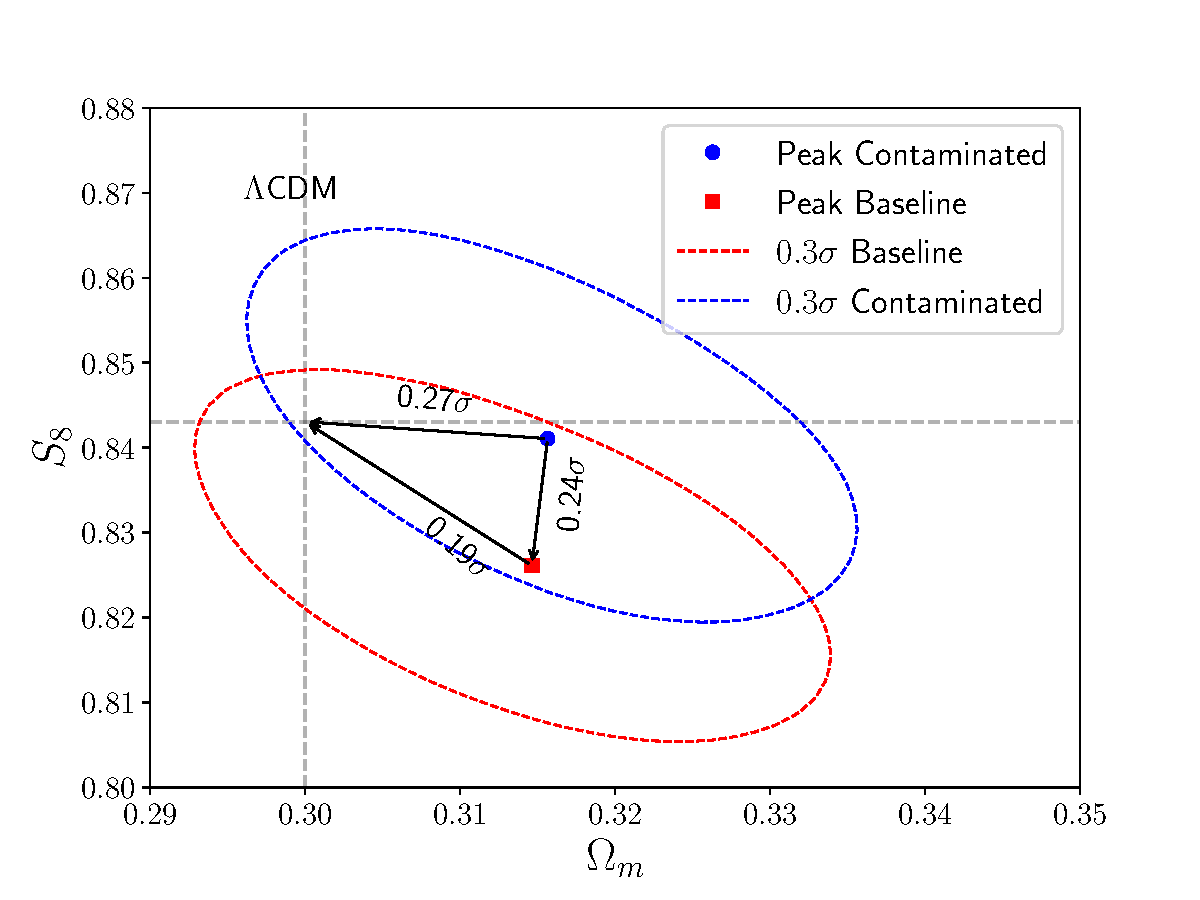
\includegraphics[width=0.49\textwidth]{figs/compare_cosmo_all_2x2pt_lcdm_sc_8_6_OmS8_draftv1.pdf}
%      }
% \hfill
% \subfloat{%
%       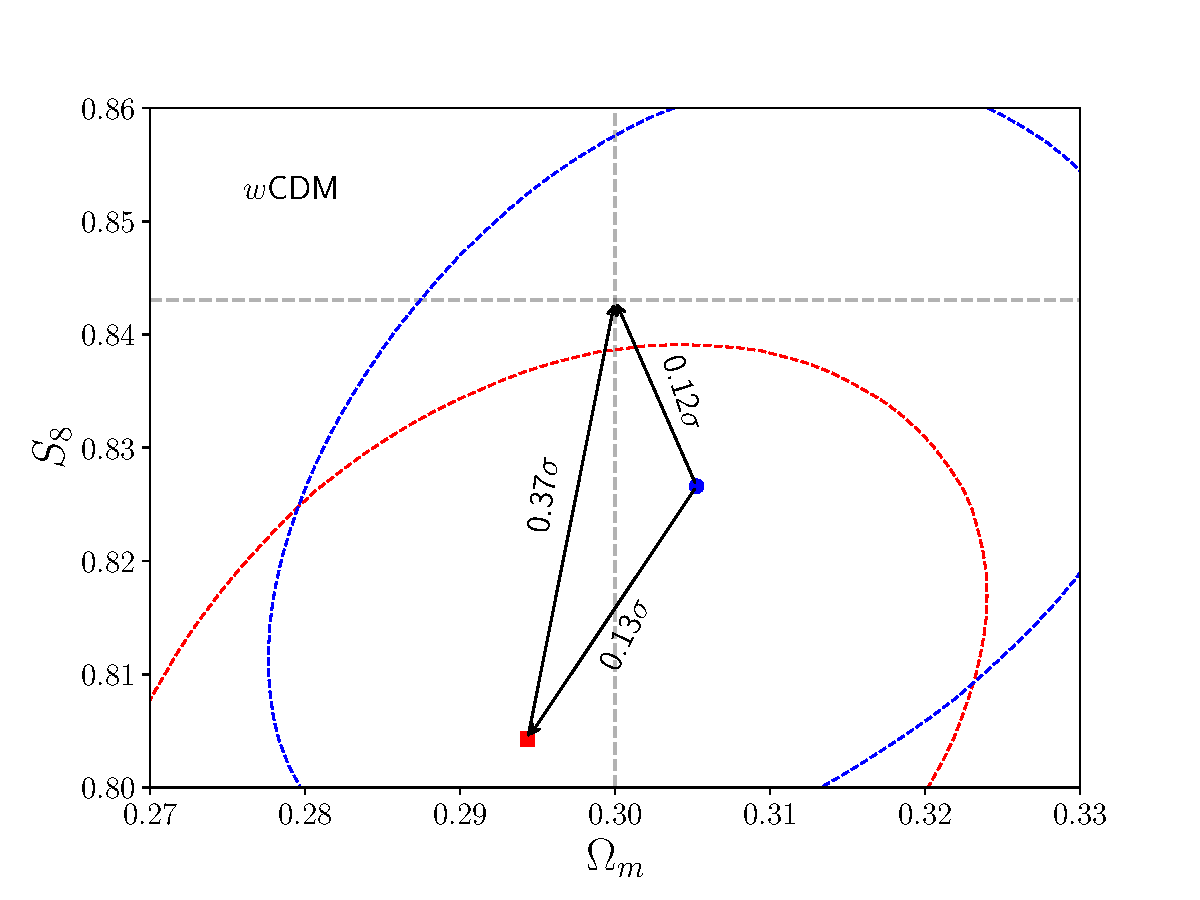
\includegraphics[width=0.49\textwidth]{figs/compare_cosmo_all_2x2pt_wcdm_sc_8_6_OmS8_draftv1.pdf}
%      }
% \vskip\baselineskip
% \subfloat{%
%       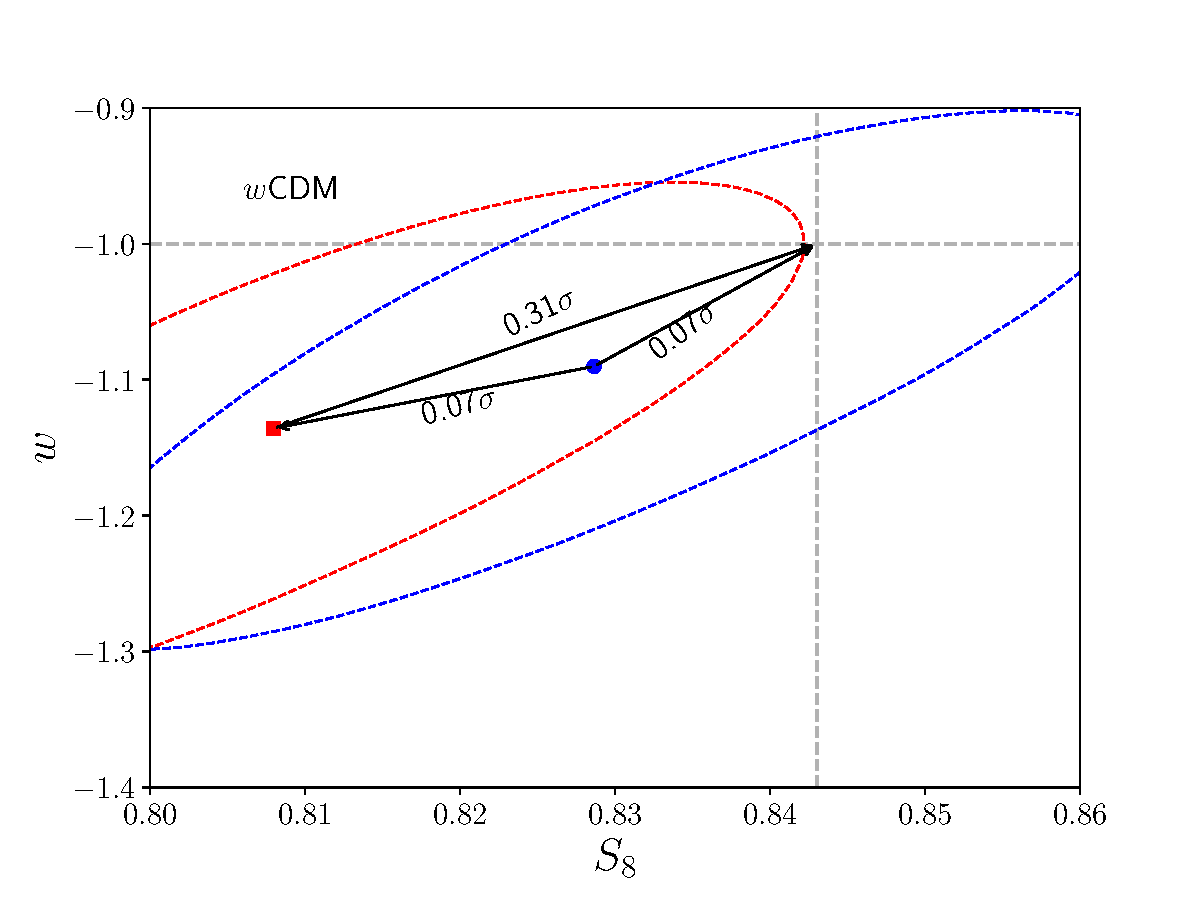
\includegraphics[width=0.49\textwidth]{figs/compare_cosmo_all_2x2pt_wcdm_sc_8_6_S8w_draftv1.pdf}
%      }
% \hfill
% \subfloat{%
%       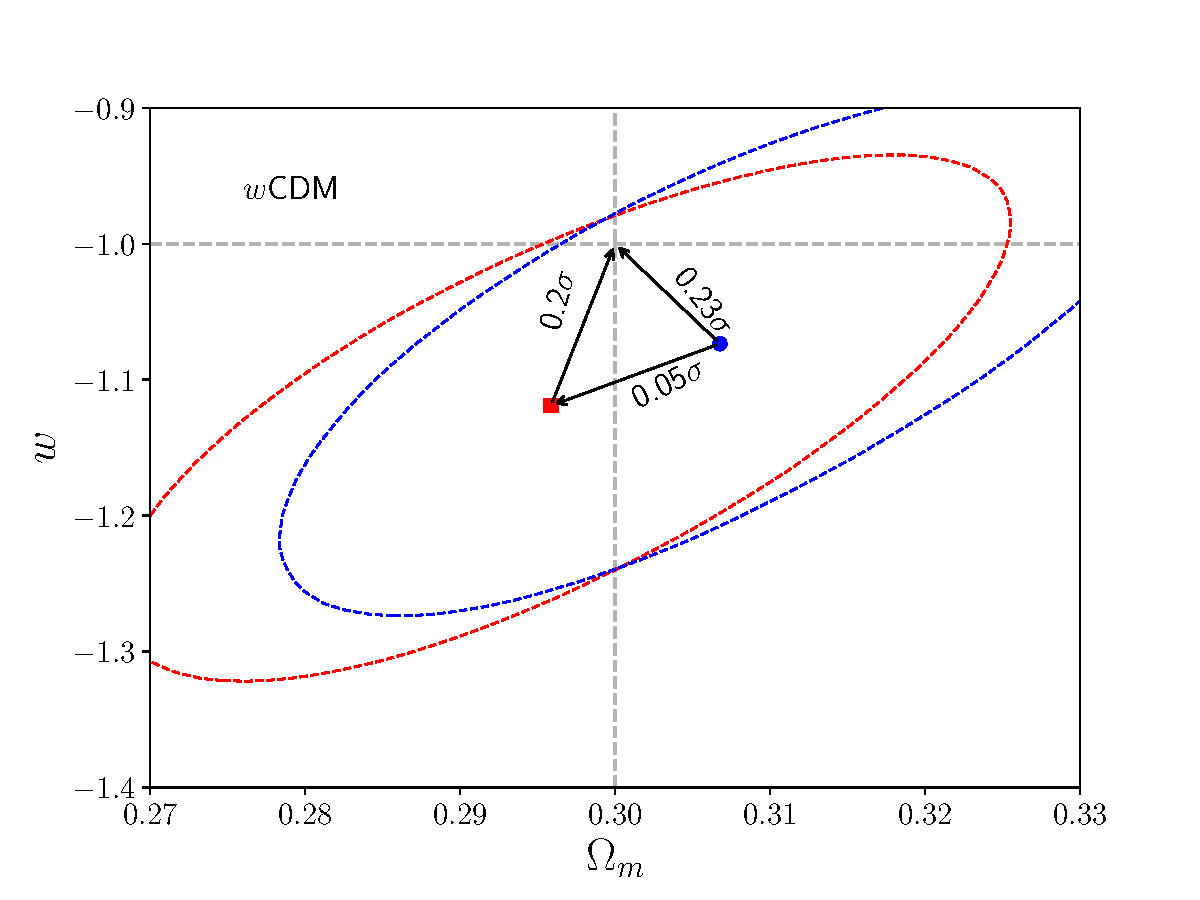
\includegraphics[width=0.49\textwidth]{figs/compare_cosmo_all_2x2pt_wcdm_sc_8_6_Omw_draftv1.pdf}
%      }
%     \caption[]{Simulated likelihood analysis when analyzing a datavector contaminated with non-linear bias + baryons and analyzed with linear bias + halofit as the model. The panels on the top-left shows contours for \lcdm cosmology while rest of the panels show \wcdm cosmology at (8,6) Mpc/$h$ scale cut for $w(\theta)$ and $\gamma_t$ respectively. In each panel we compare the peak of the marginalized constraints in the 2D cosmological parameters plane when analyzing the contaminated datavector (blue circle) and the baseline datavector with zero contamination (red square). We see that the distance of the peak of marginalized baseline contours is within 0.3$\sigma$ of marginalized contaminated contours which is our threshold criteria for finding the minimum acceptable scales to be used for cosmological analysis.}
% \end{figure*}

\begin{figure*}
\centering
\subfloat{%
       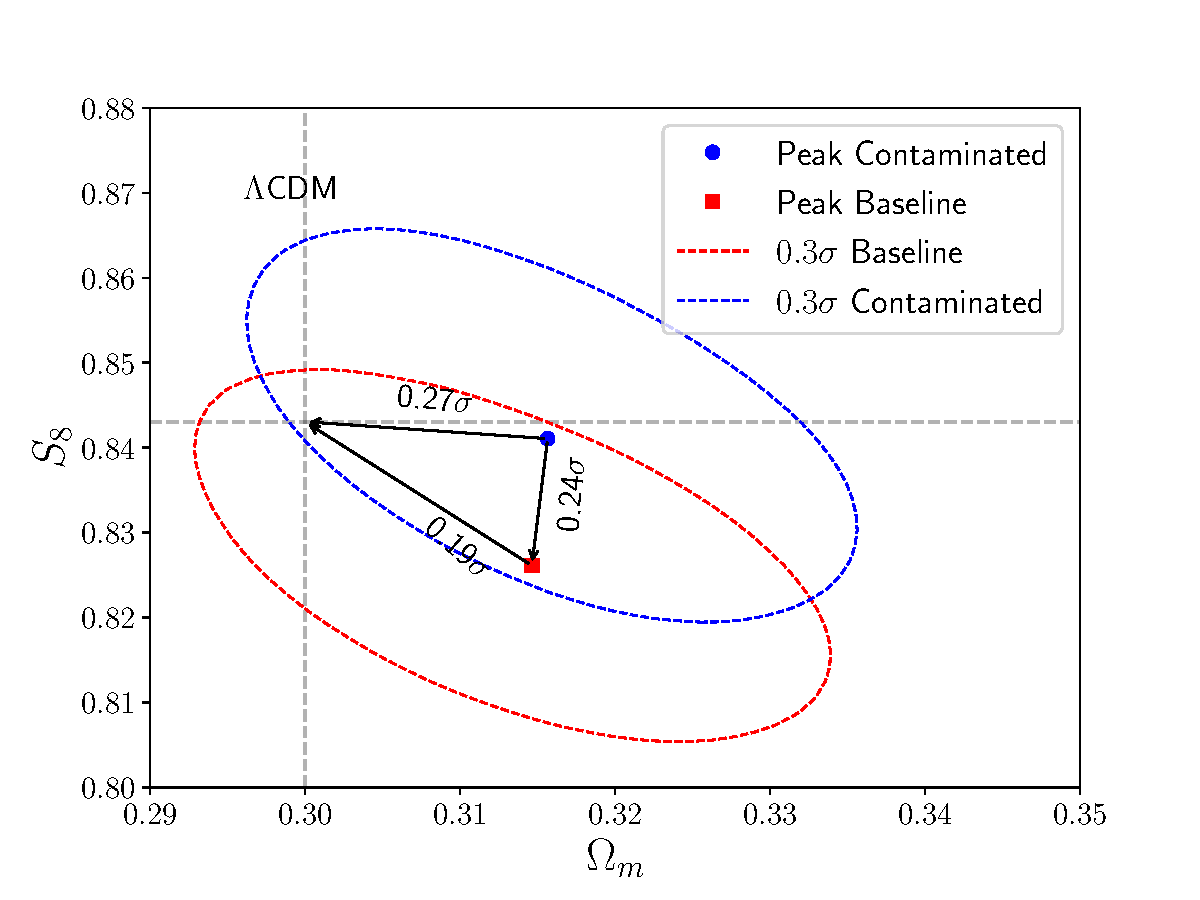
\includegraphics[width=0.49\textwidth]{figs/compare_cosmo_all_2x2pt_lcdm_sc_8_6_OmS8_draftv1.pdf}
     }
\hfill
\subfloat{%
      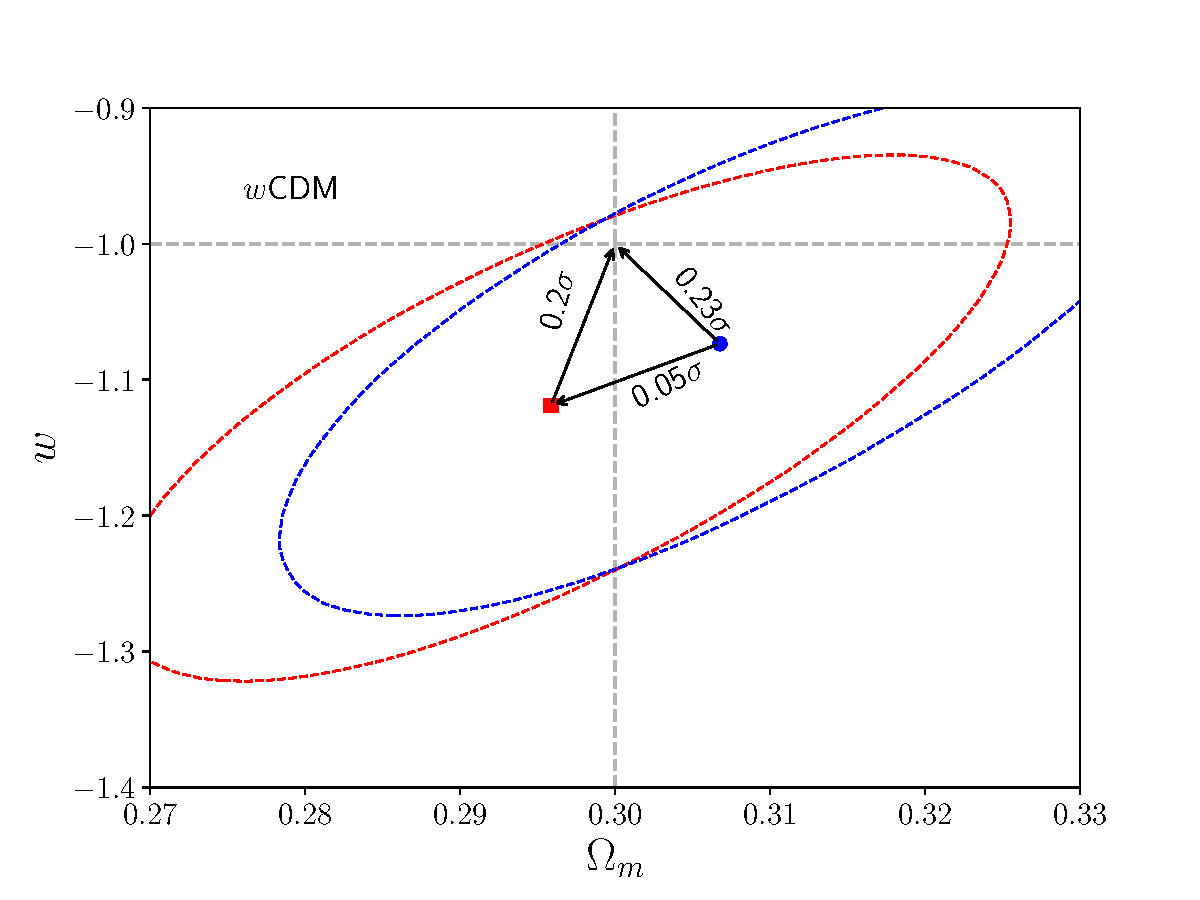
\includegraphics[width=0.49\textwidth]{figs/compare_cosmo_all_2x2pt_wcdm_sc_8_6_Omw_draftv1.pdf}
     }
    \caption[]{Simulated likelihood analysis: results show the analysis of a datavector contaminated with non-linear bias + baryons analyzed with a linear bias + halofit model. The left panel   shows contours for \lcdm  and the right panel shows \wcdm. The scale cuts are (8,6) Mpc/$h$ for $w(\theta)$ and $\gamma_t$ respectively. In both panels we compare the peak of the marginalized constraints in the 2D  parameter plane for the contaminated datavector (blue circle) and the baseline datavector  (red square). We see that the distance between the peaks of marginalized baseline contours is within 0.3$\sigma$ of the marginalized contaminated contours, which is our  criterion for acceptable scale cuts. }
\end{figure*}


% \begin{figure*}
% 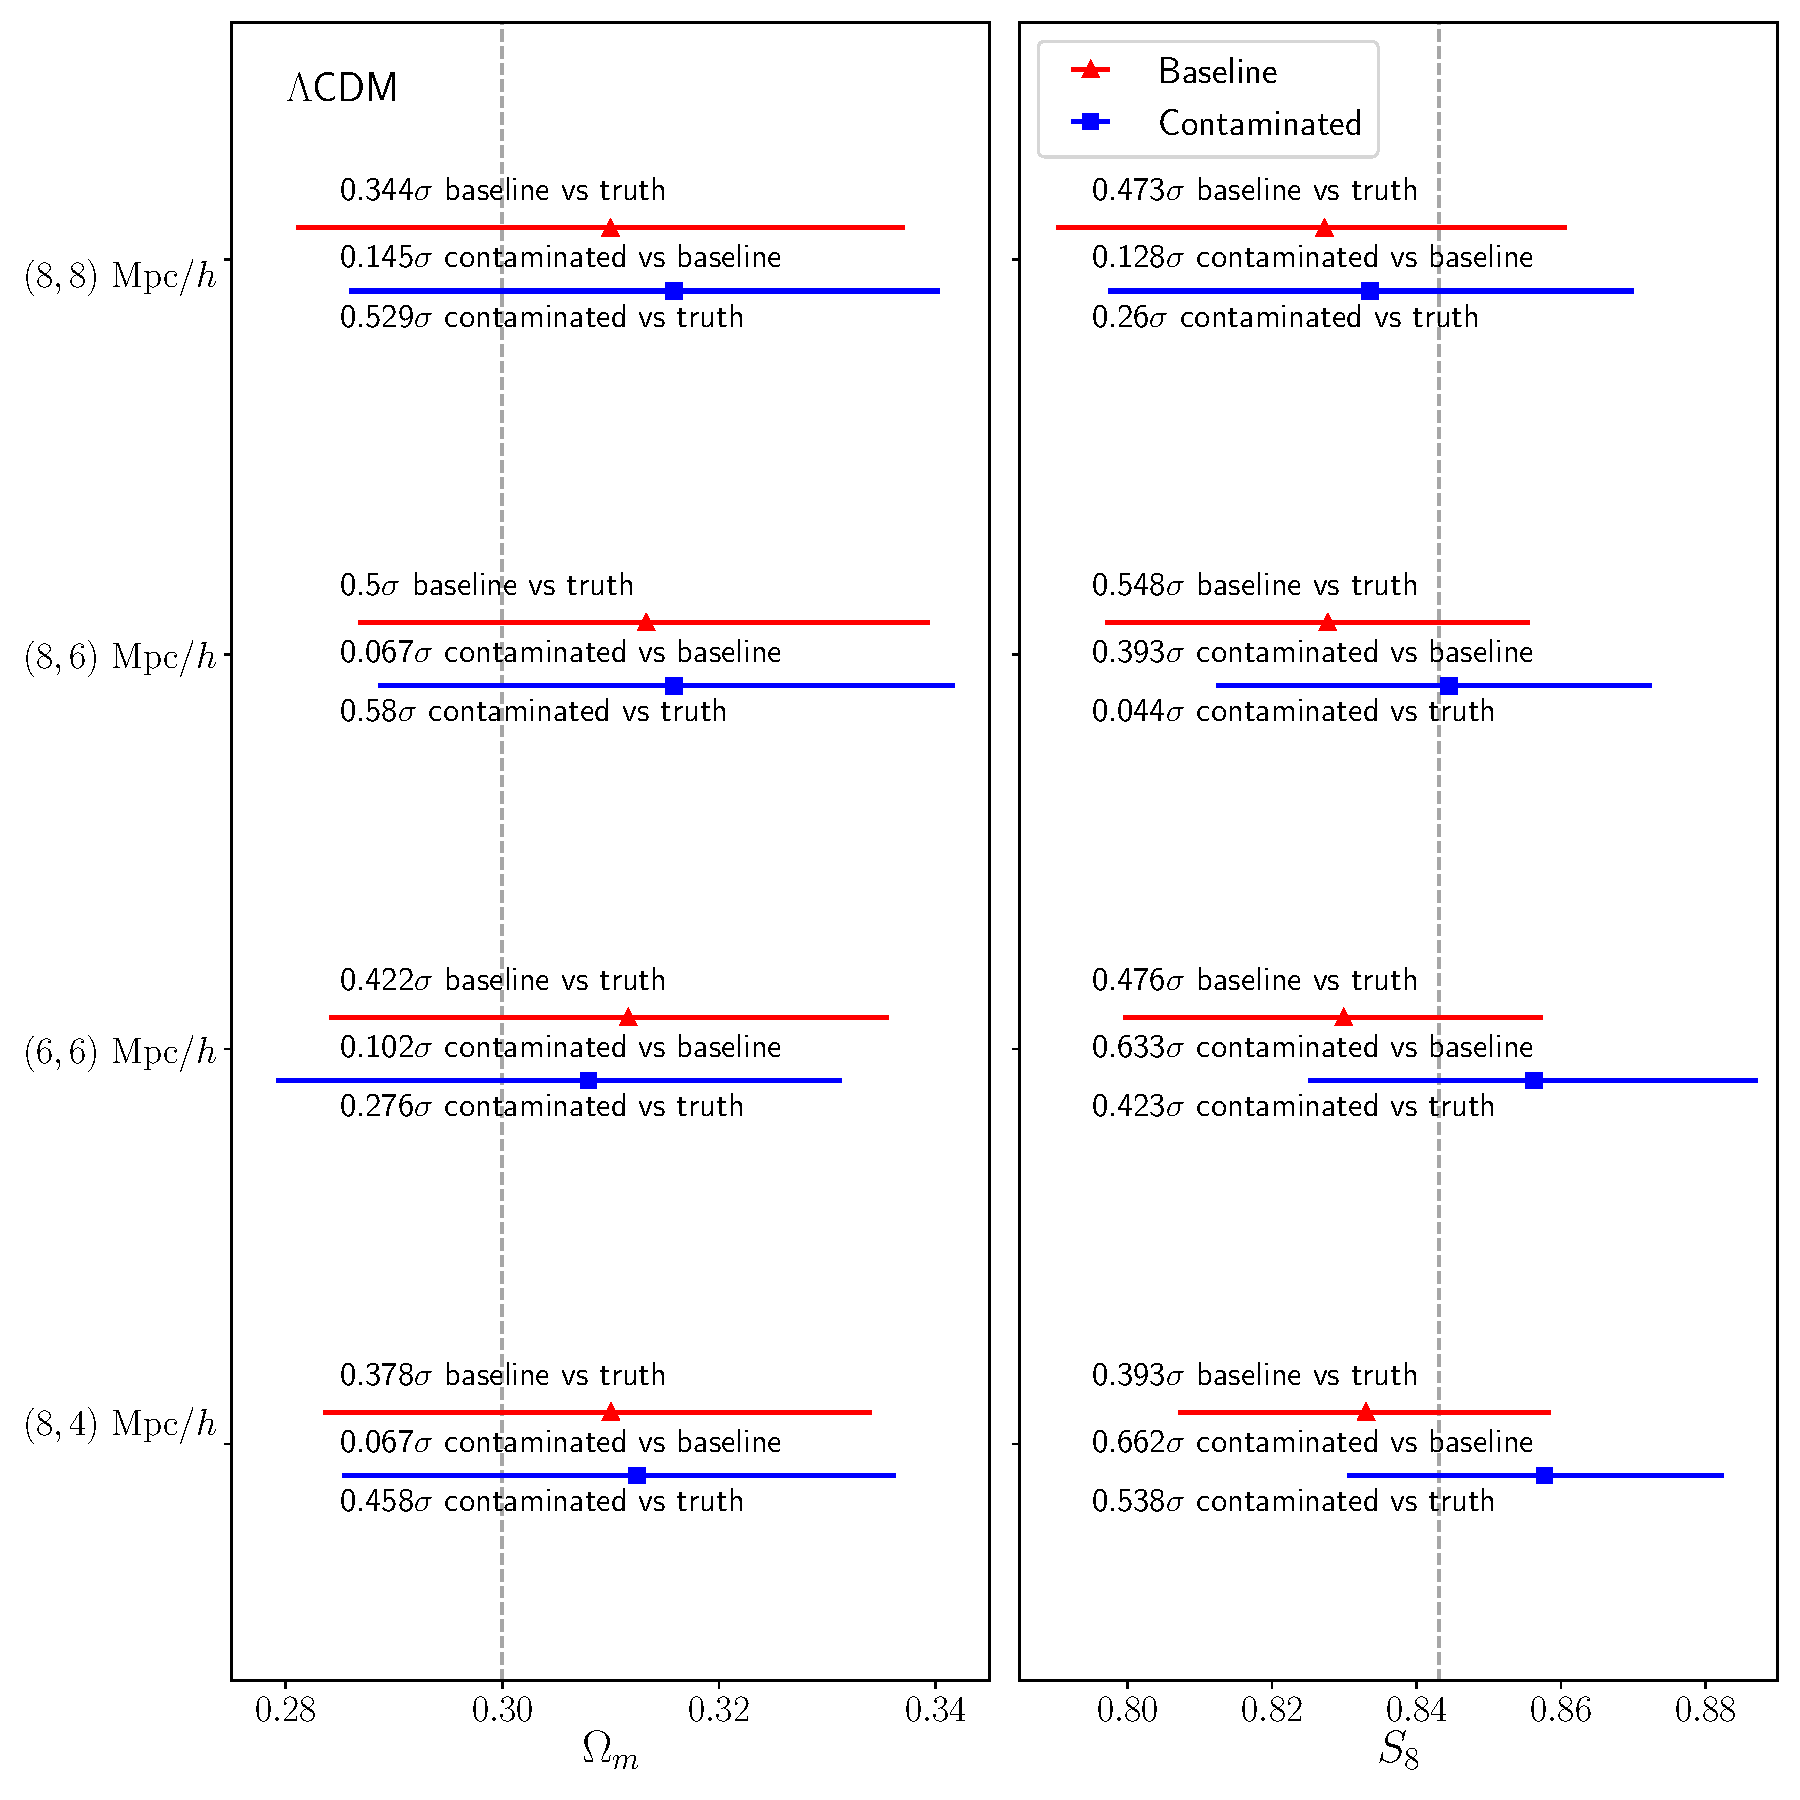
\includegraphics[width=\columnwidth]{figs/2x2pt_1dmarg_lcdm_paper.pdf}
% 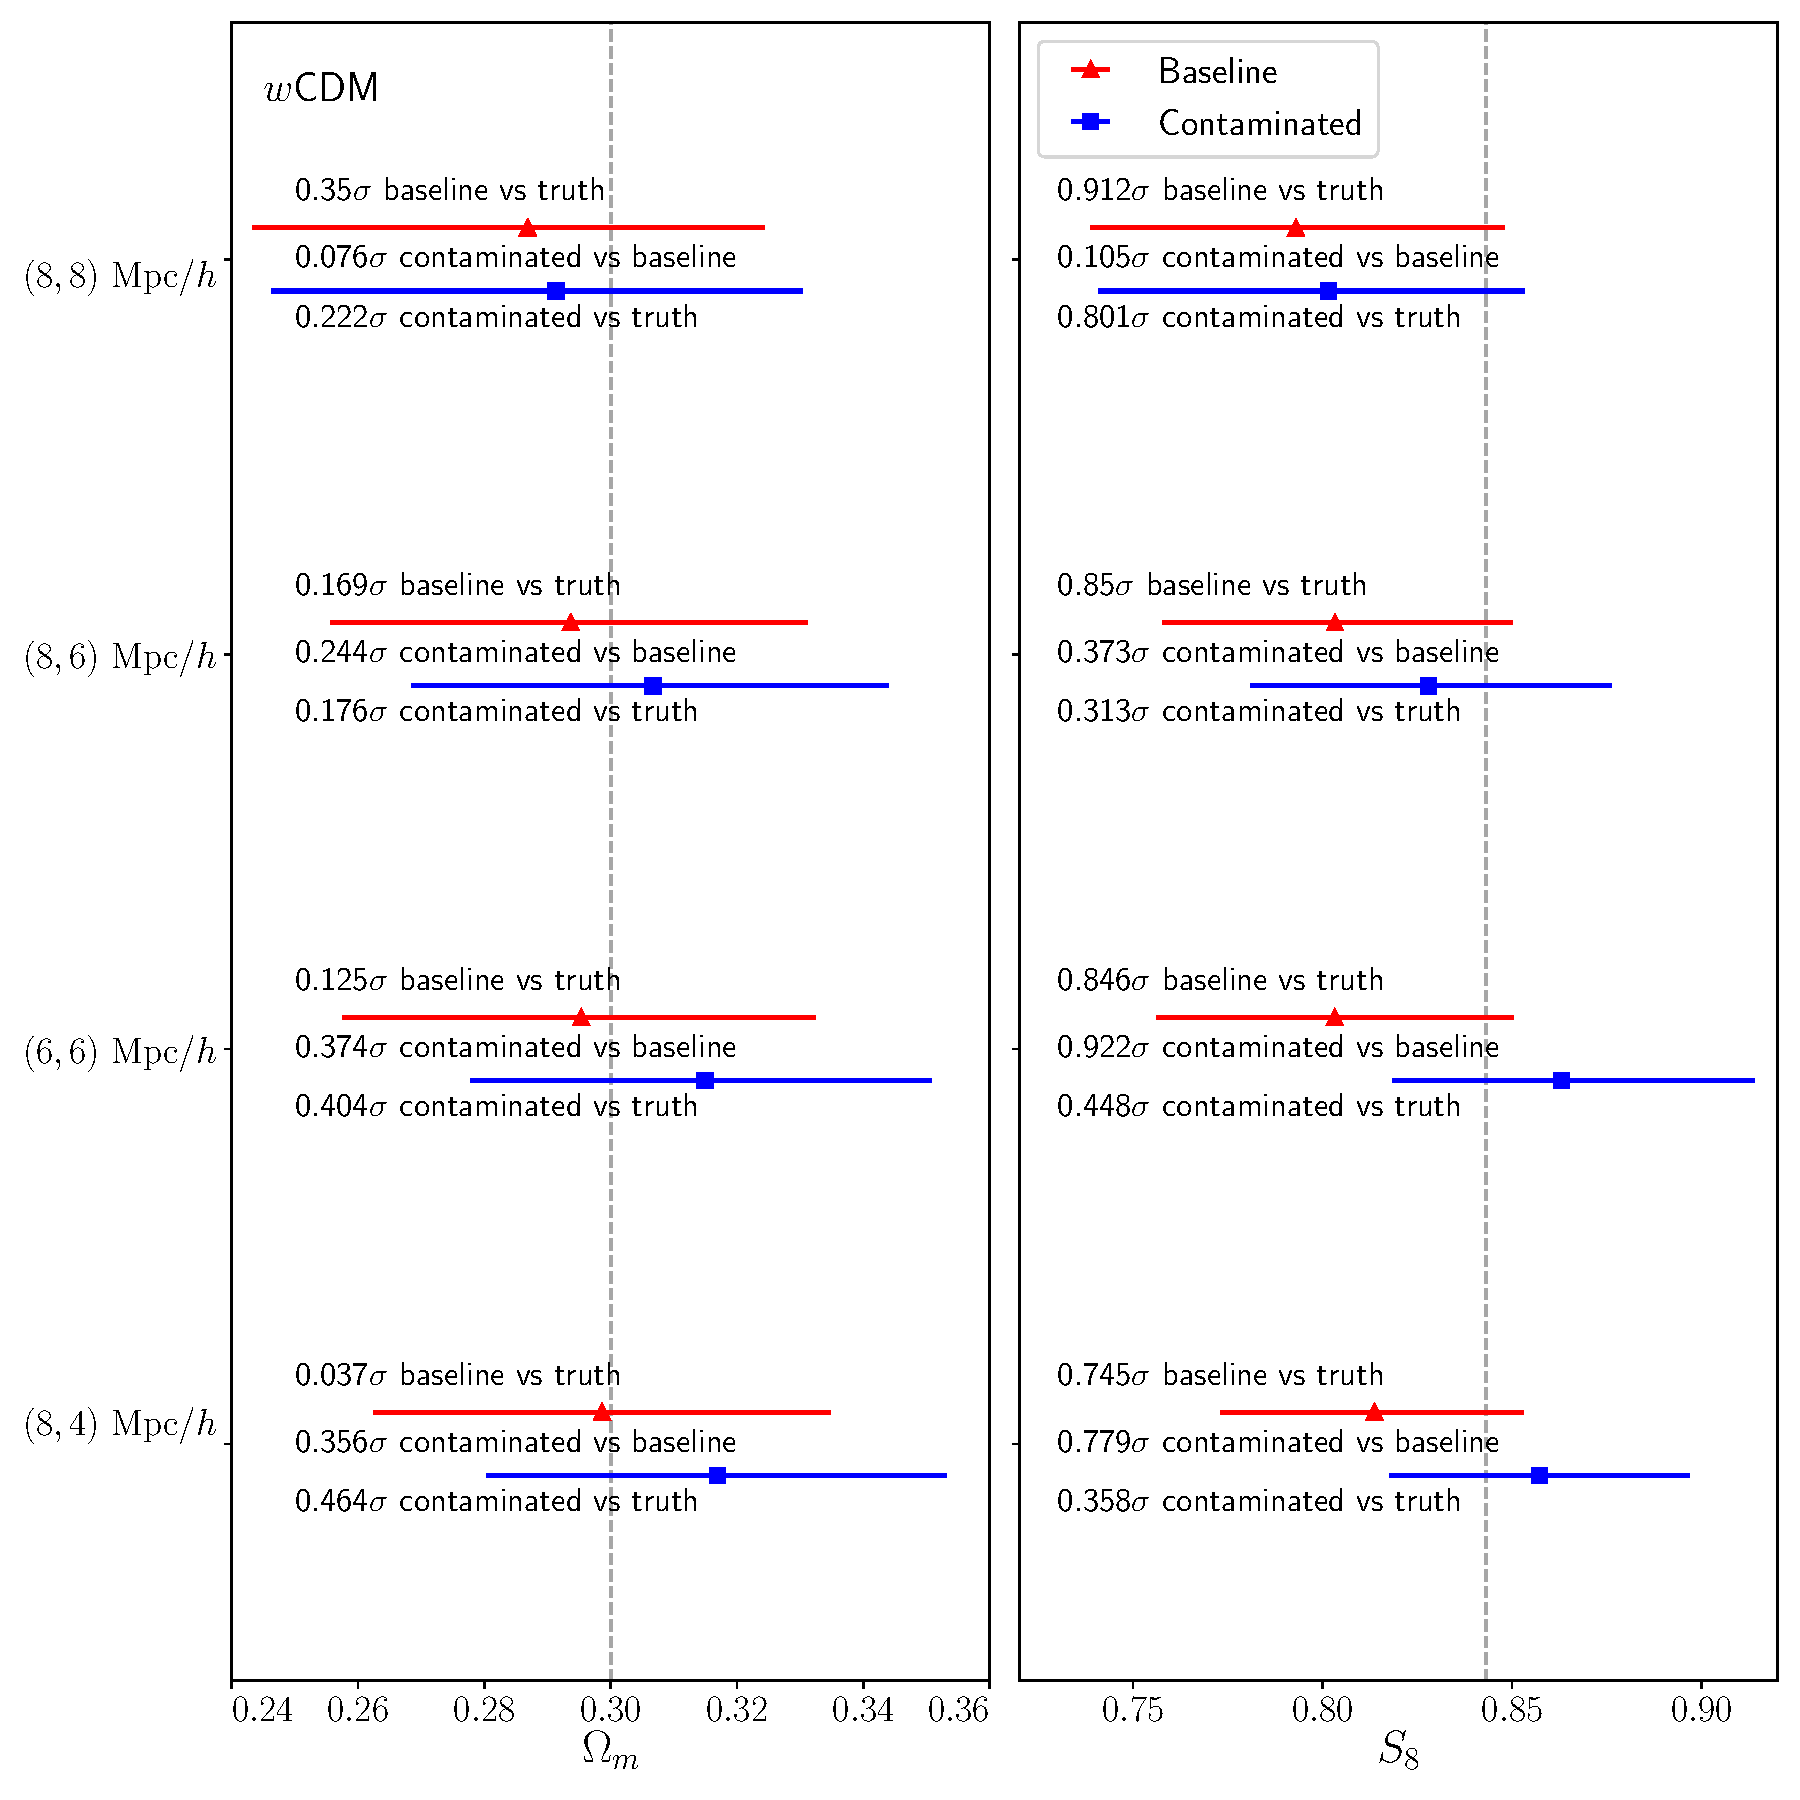
\includegraphics[width=\columnwidth]{figs/2x2pt_1dmarg_wcdm_paper.pdf}
% \caption[]{Simulated likelihood analysis when analyzing a datavector contaminated with non-linear bias + baryons and analyzed with linear bias + halofit as the model. The two panels on the left show \lcdm while the panels on the right show \wcdm. For each scale cut for (\wtheta,\gammat) as indicated on the y-axis labels, we compare the recovered cosmological  constraints for the contaminated datavector and baseline datavector (with zero contamination). There are residual biases in both $\Omega_m$ and $S_8$ even in baseline case (due to projection effects, see \S\ref{sec:simlike_analysis} and Appendix \ref{app:projection_effects}), the difference between constraints from the baseline and contaminated datavector gets larger as we go down in scale cuts along y-axis. We use the criterion of difference between contaminated and baseline being greater than X$\sigma$, to choose our fiducial scale cuts for the linear bias model as (X,Y)Mpc/$h$.    }
% \label{fig:sim_lin}
% \end{figure*}




\subsection{Results on Simulations}

For  analysis choice combinations that pass the simulated likelihood tests, we then validate with mock catalogs from cosmological simulations: the suite of Y3 \buzzard simulations are shown here. We again require that our analysis choices  return unbiased cosmological parameters. In order to reduce the sample variance we analyze the mean datavector constructed from 18 \buzzard realizations. \red{Mention that we analyze the \mice sims as well but that has only one realizations. The recovered cosmological contours and bestfit are shown in Appendix XXX}.

\subsubsection{Linear Bias Model}
We have run simulated $2\times 2$-point analyses on the mean of the measurements from all 18 simulations. We compare our model for $w(\theta)$ and $\gamma_t(\theta)$ to our measurements at the true \textsc{Buzzard} cosmology leaving only linear bias and magnification coefficients free, totaling 10 free parameters, and find a chi-squared value of 44.9 for 285 data points using our fiducial scale cuts and assuming the covariance of a single simulation. Simulated analyses assuming the true simulated source redshift distributions and the fiducial model described in Sec. \ref{sec:model}, but fixing source redshift uncertainties to zero results in cosmological constraints that have a probability to exceed a parameter bias of $0.3/1\sigma$ in the $S_8-\Omega_{m}$ plane of XXX/$<$0.001. A similar analysis, using calibrated photometric redshift distributions rather than true redshift distributions shows a probability to exceed a parameter bias of $0.3/1\sigma$ in the $S_8-\Omega_{m}$ plane with respect to the true redshift analysis of XXX/0.002.

\subsubsection{Scale cuts for non-linear bias}
Likewise we have run simulated $2\times 2$-point analyses including our non-linear bias model on the mean of the measurements from all 18 simulations. We compare our model for $w(\theta)$ and $\gamma_t(\theta)$ to our measurements at the true \textsc{Buzzard} cosmology leaving our bias model parameters and magnification coefficients free, totaling 15 free parameters, and find a chi-squared value of \jdr{XXX} for \jdr{XXX to be determined once we decide on scale cuts} data points using our non-linear bias scale cuts and assuming the covariance of a single simulation. Simulated analyses using true redshift distributions result in cosmological constraints that have a probability to exceed a parameter bias of $0.3/1\sigma$ in the $S_8-\Omega_{m}$ plane of XXX/$<$0.001. 

% \subsubsection{Cosmological constraints}

% \begin{figure*}
% 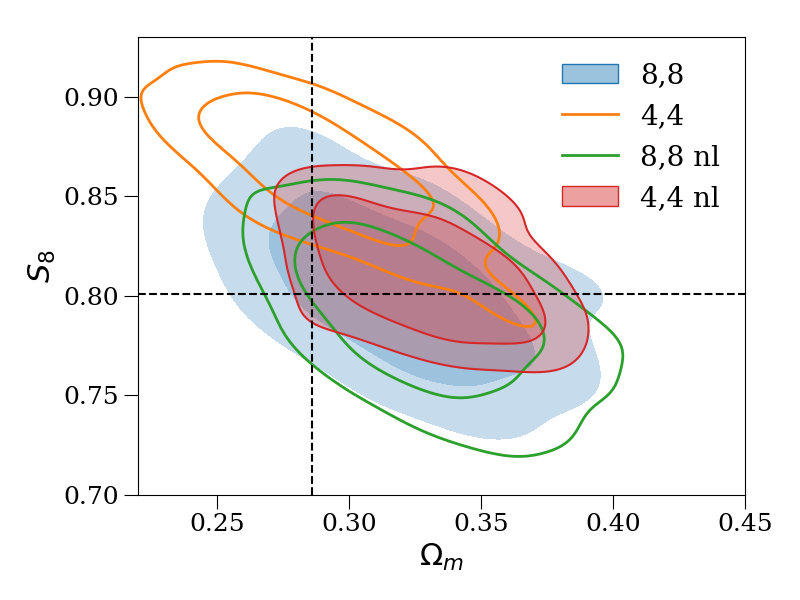
\includegraphics[width=\columnwidth]{figs/buzzard_lcdm_om-s8.png}
% 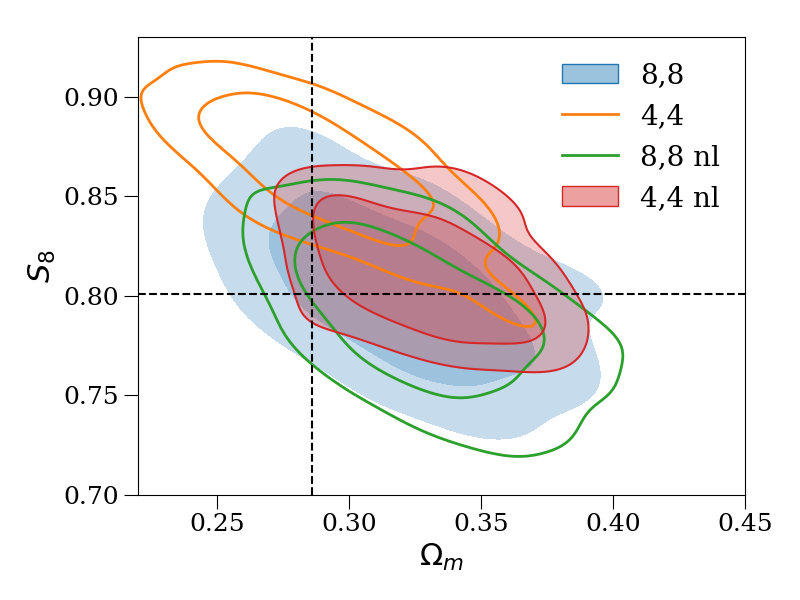
\includegraphics[width=\columnwidth]{figs/buzzard_lcdm_om-s8.png}
% \caption[]{\lcdm\ Buzzard constraints, we show the constraints on $\Omega_m$ and $S_8$ from the mean (over all N realizations) Buzzard 2x2pt measurements, with cosmological parameter priors set I (i.e. wide, ~uninformative priors) in the left panel, and set II in the right panel. We show constraints with two sets of scale cuts: 4,4 and 8,6. In each panel we show constraints for linear and non-linear galaxy bias models. Comment on which of the options give unbiased cosmology. Use this figure to set the scale cuts for non-linear bias model as well.  }
% \label{fig:bcc_des_lcdm}
% \end{figure*}


\begin{figure*}
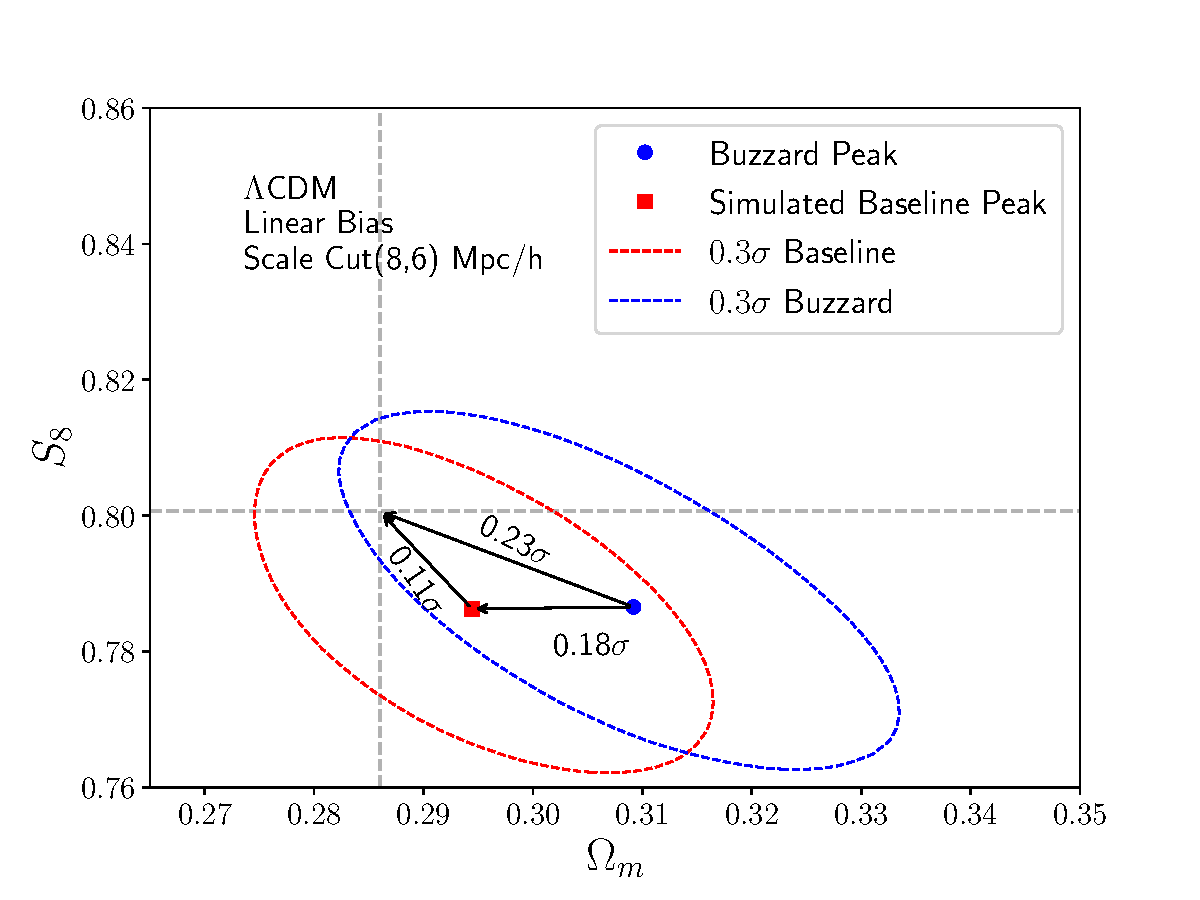
\includegraphics[width=\columnwidth]{figs/linear_bias_86_lcdm_Om_S8_buzzard.pdf}
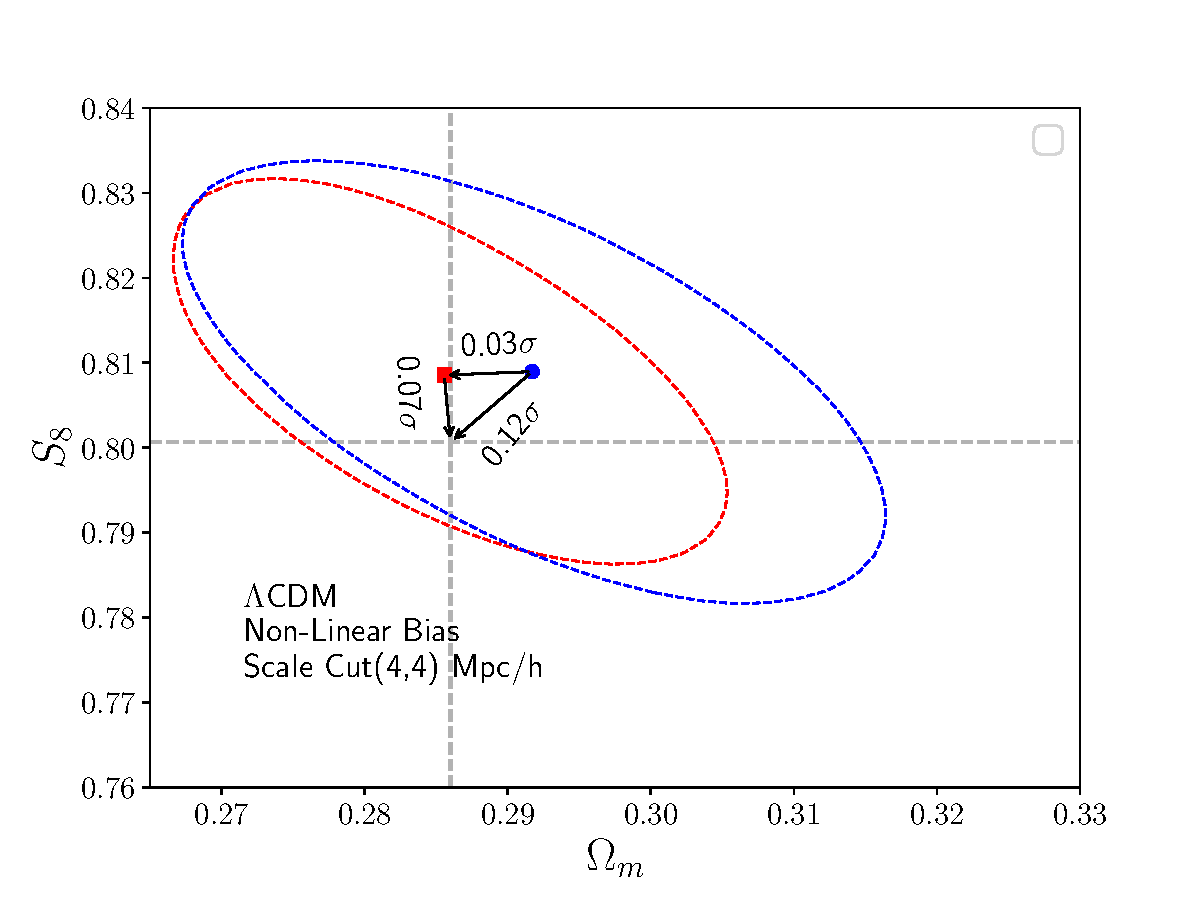
\includegraphics[width=\columnwidth]{figs/non_linear_bias_44_lcdm_Om_S8_buzzard.pdf}
\caption[]{\lcdm\ Buzzard constraints (blue contours) compared with  Buzzard-like theory datavector (red contours). The blue contours correspond to the result from the mean (over all Y3-like realizations) of Buzzard 2x2pt measurements, with covariance corresponding to single realization. The left (right) panel shows the constraints for linear (nonlinear) bias models  with the scale cuts given in the legend. The linear and non-linear bias values are extracted from fits to the 3D correlation functions ($\xigg$ and $\xigm$). We see that both  the scale cut choices satisfy our validation criterion. }
\label{fig:bcc_des_lcdm}
\end{figure*}

In \fig{fig:bcc_des_lcdm} we show the constraints on $\Omega_m$ and $S_8$ from the mean Buzzard 2x2pt measurements for \lcdm. The results for the linear and nonlinear bias models are shown, and again, the criterion for unbiased cosmology is satisfied for the fiducial choice of scale cuts. 
\fig{fig:bcc_des_wcdm} shows the same analysis for $\Omega_m$ and $w$.


%\subsubsection{DES-only $\wcdm$ and DES + Planck $\wcdm$}

% \begin{figure*}
% 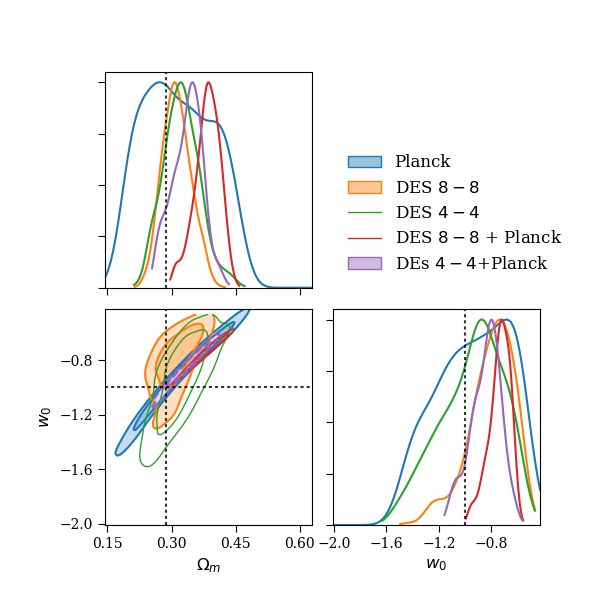
\includegraphics[width=\columnwidth]{figs/buzzard_wcdm_lin_om-w.png}
% 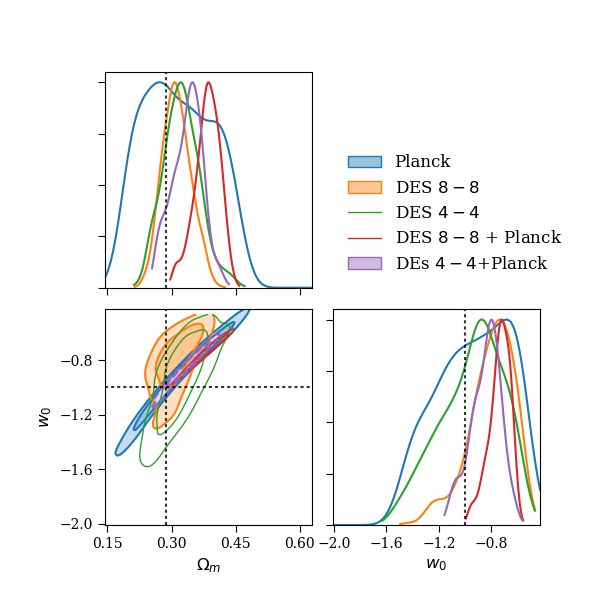
\includegraphics[width=\columnwidth]{figs/buzzard_wcdm_lin_om-w.png}
% \caption[]{\wcdm\ Buzzard constraints, linear bias (left panel), non-linear bias (right-panel). Show the constraints with DES alone as well as when using with Planck.}
% \label{fig:color_ims}
% \end{figure*}

\begin{figure*}
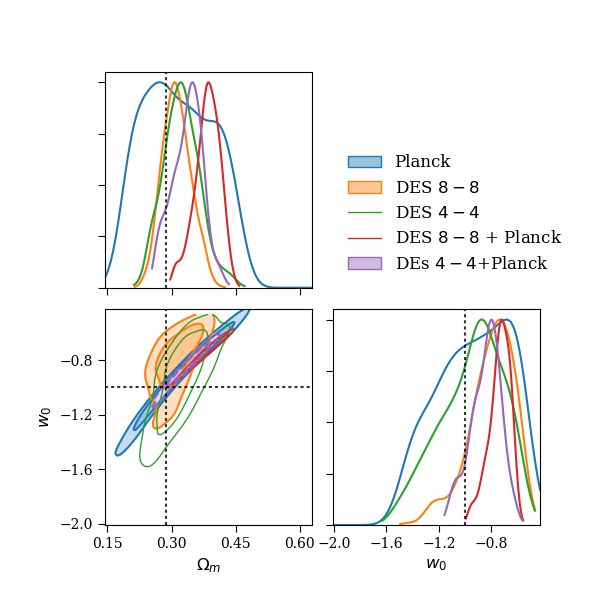
\includegraphics[width=\columnwidth]{figs/buzzard_wcdm_lin_om-w.png}
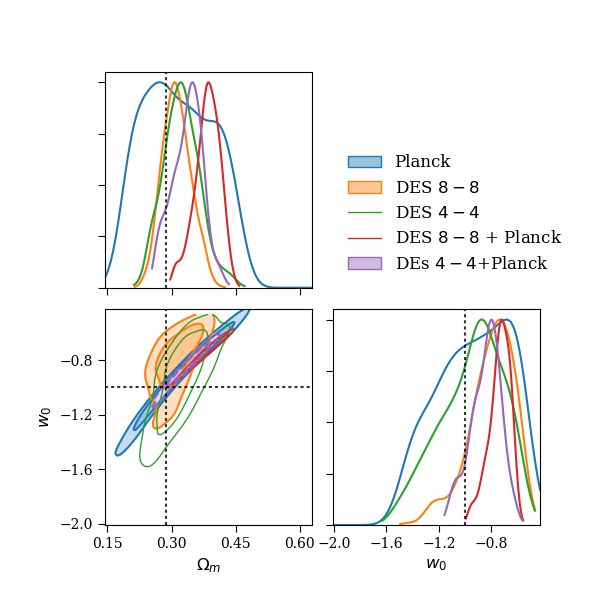
\includegraphics[width=\columnwidth]{figs/buzzard_wcdm_lin_om-w.png}
\caption[]{Same as Fig.~\ref{fig:bcc_des_lcdm} but for $w$CDM cosmology.}
\label{fig:bcc_des_wcdm}
\end{figure*}


Also validate bias modelling choices at fixed cosmology?

\red{Mention that the results for $\mice$ sims are in the appendix}


\section{Results}

\subsection{DES-only constraints}

\red{Compare DES-only constraints for the analysis variations. Hopefully they agree. Compare performance of different models and present fiducial constraint.}



% \SP{\begin{itemize}
%     \item \textbf{\textit{Figure}} Compare the constraints from cosmic shear, 2x2pt and 3x2pt datavectors for the scale cuts defined for the 3x2pt $\Lambda$CDM analysis. Explain the loss of constraining power in 2x2pt compared to 3x2pt due to PM. Show for both linear bias and non-linear bias. 
% \end{itemize}
% }




\begin{figure}
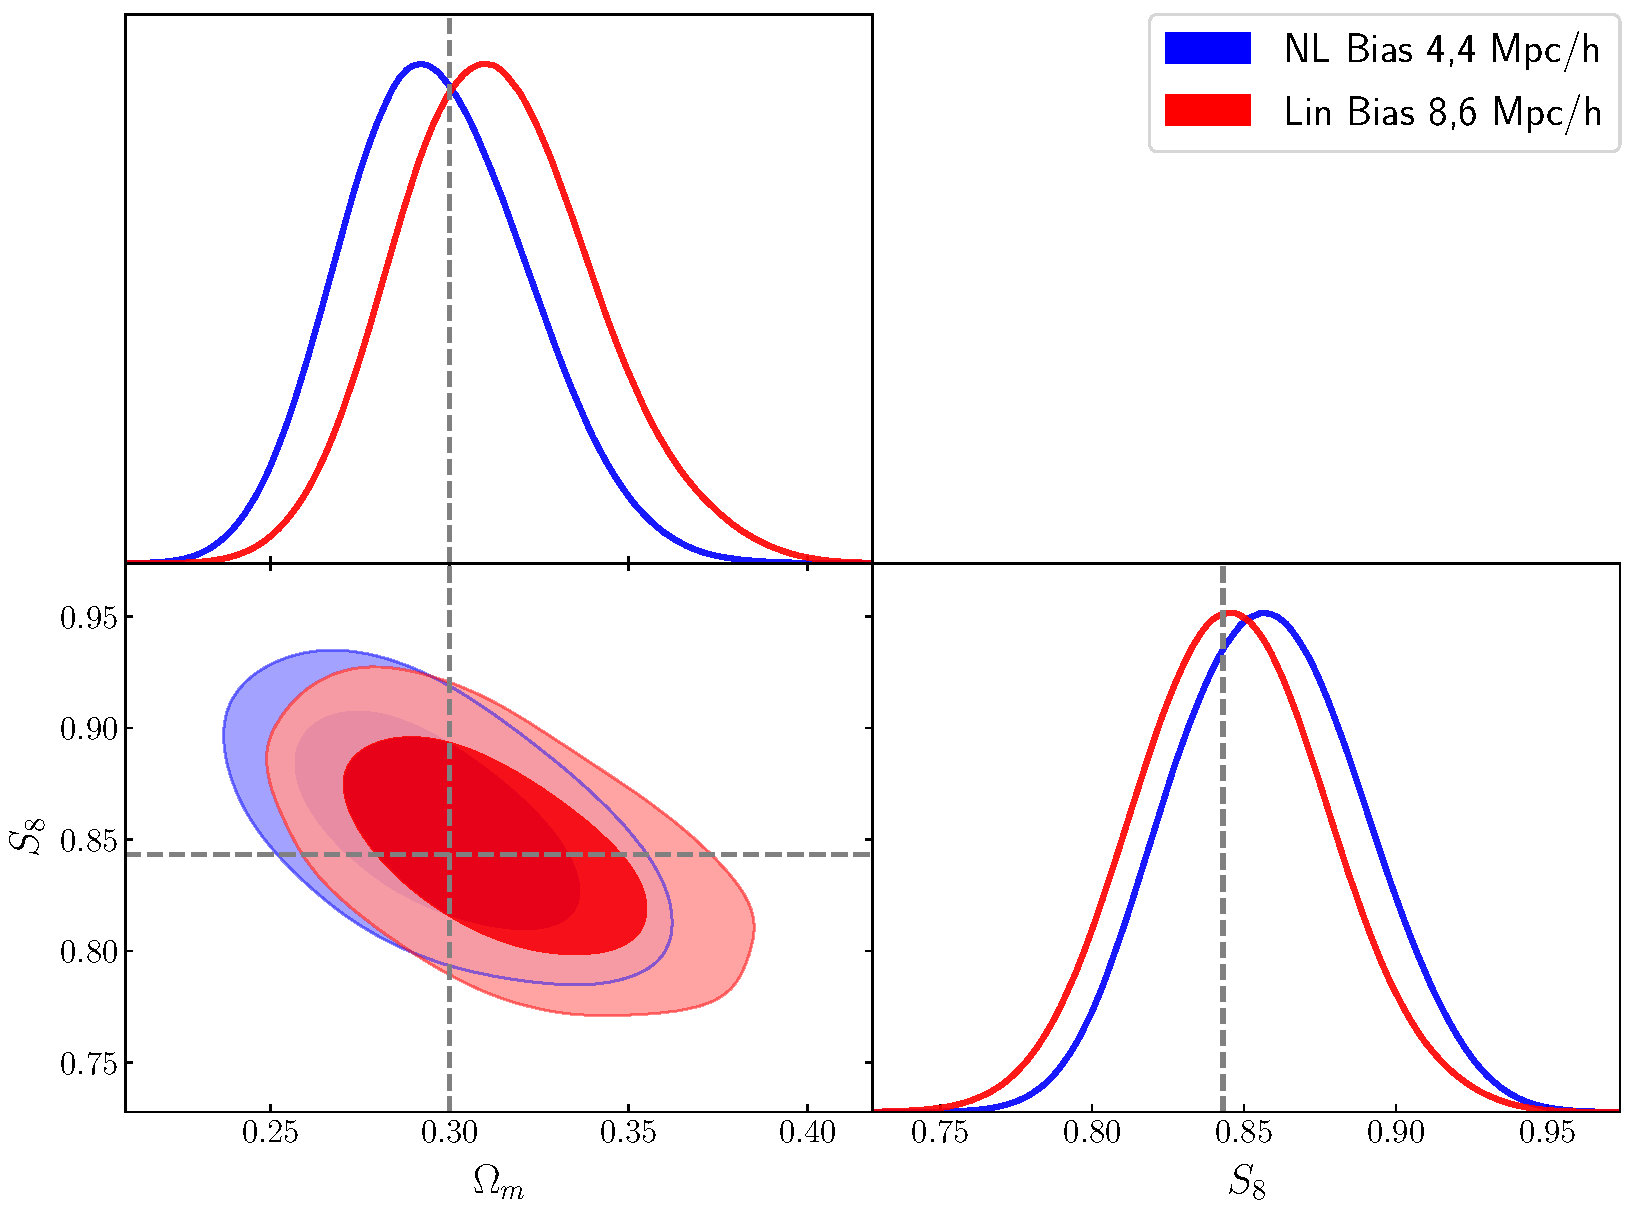
\includegraphics[width=\columnwidth]{figs/compare_cosmo_nl44_lin86.pdf}
\caption[]{DATA: Compare the 2x2pt $\Lambda$CDM and $w$CDM constraints for both linear bias and non-linear bias at their respectively defined scale cuts with DES only. We show that using non-linear bias leads to more constraining power, especially in $\Omega_m$, with the ability to push down to smaller scales.  \SP{also will add (8,6) scale cut contour for non-linear bias model and the $w$CDM contours in another panel. Comment on why (because of PM marginalization) the gain is rather small in 2x2pt but we expect big gain for 3x2pt.} }
\label{fig:des_comp}
\end{figure}


\subsection{DES+Planck constraints}

\red{Cosmology and galaxy bias constraints from DES+external. Again compare performance of different analysis choices. Compare bias constraints with some theoretical expectations.}

\begin{figure}
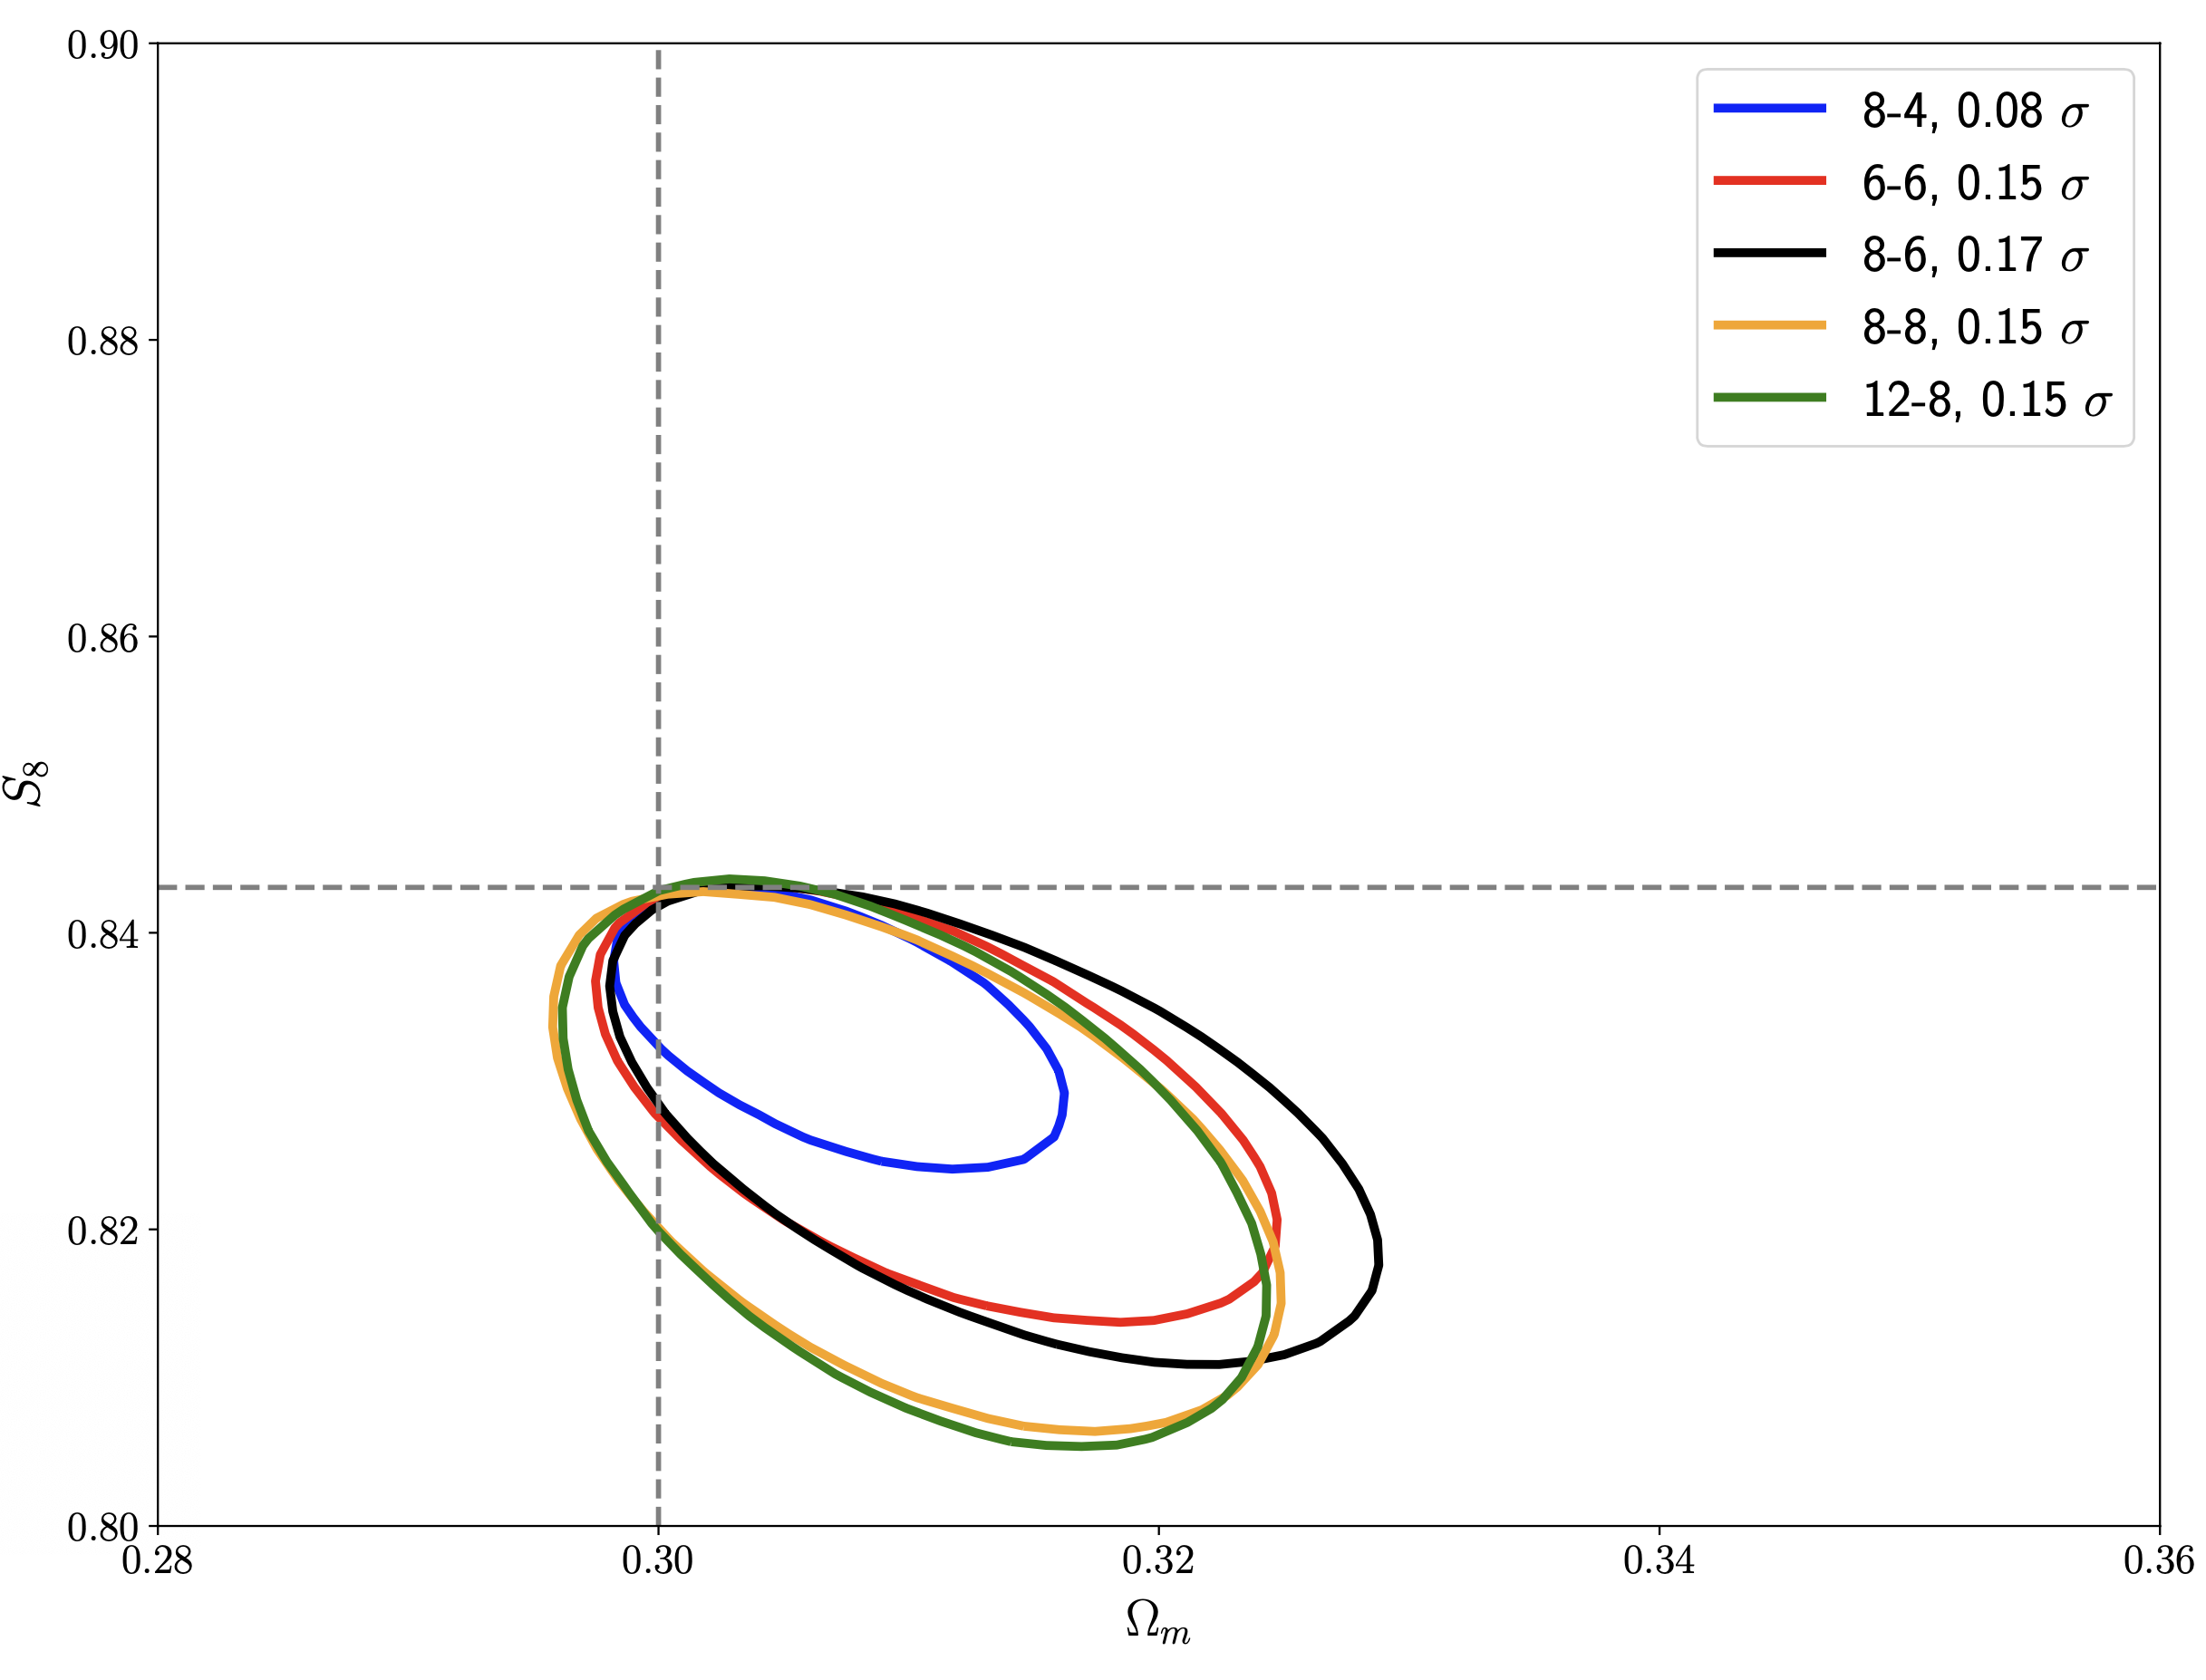
\includegraphics[width=\columnwidth,draft]{figs/temp.png}
\caption[]{DATA: Show the DES+external constraints for both \lcdm \ and \wcdm \ cosmologies. Show DES and external alone and their combination. Comment of their consistency and on their tension. }
\label{fig:bias_relation}
\end{figure}

\subsection{Consistency with external datasets}
\red{Which external datasets to include?}

\subsubsection{Tension metric}

\subsubsection{Results}



\subsection{Galaxy bias}
\red{Show the constraints on the galaxy bias as a function of redshifts. }
\red{Show the comparison with predictions from few different HOD models and hence infer some sort of mean halo mass constraints}
\red{Need to show the robustness of inferred masses with respect to assumed HOD form etc}
\red{Note the degeneracy between the bias and PM parameter. Note that this degeneracy will be broken in the 3x2pt analysis.}
\begin{figure}
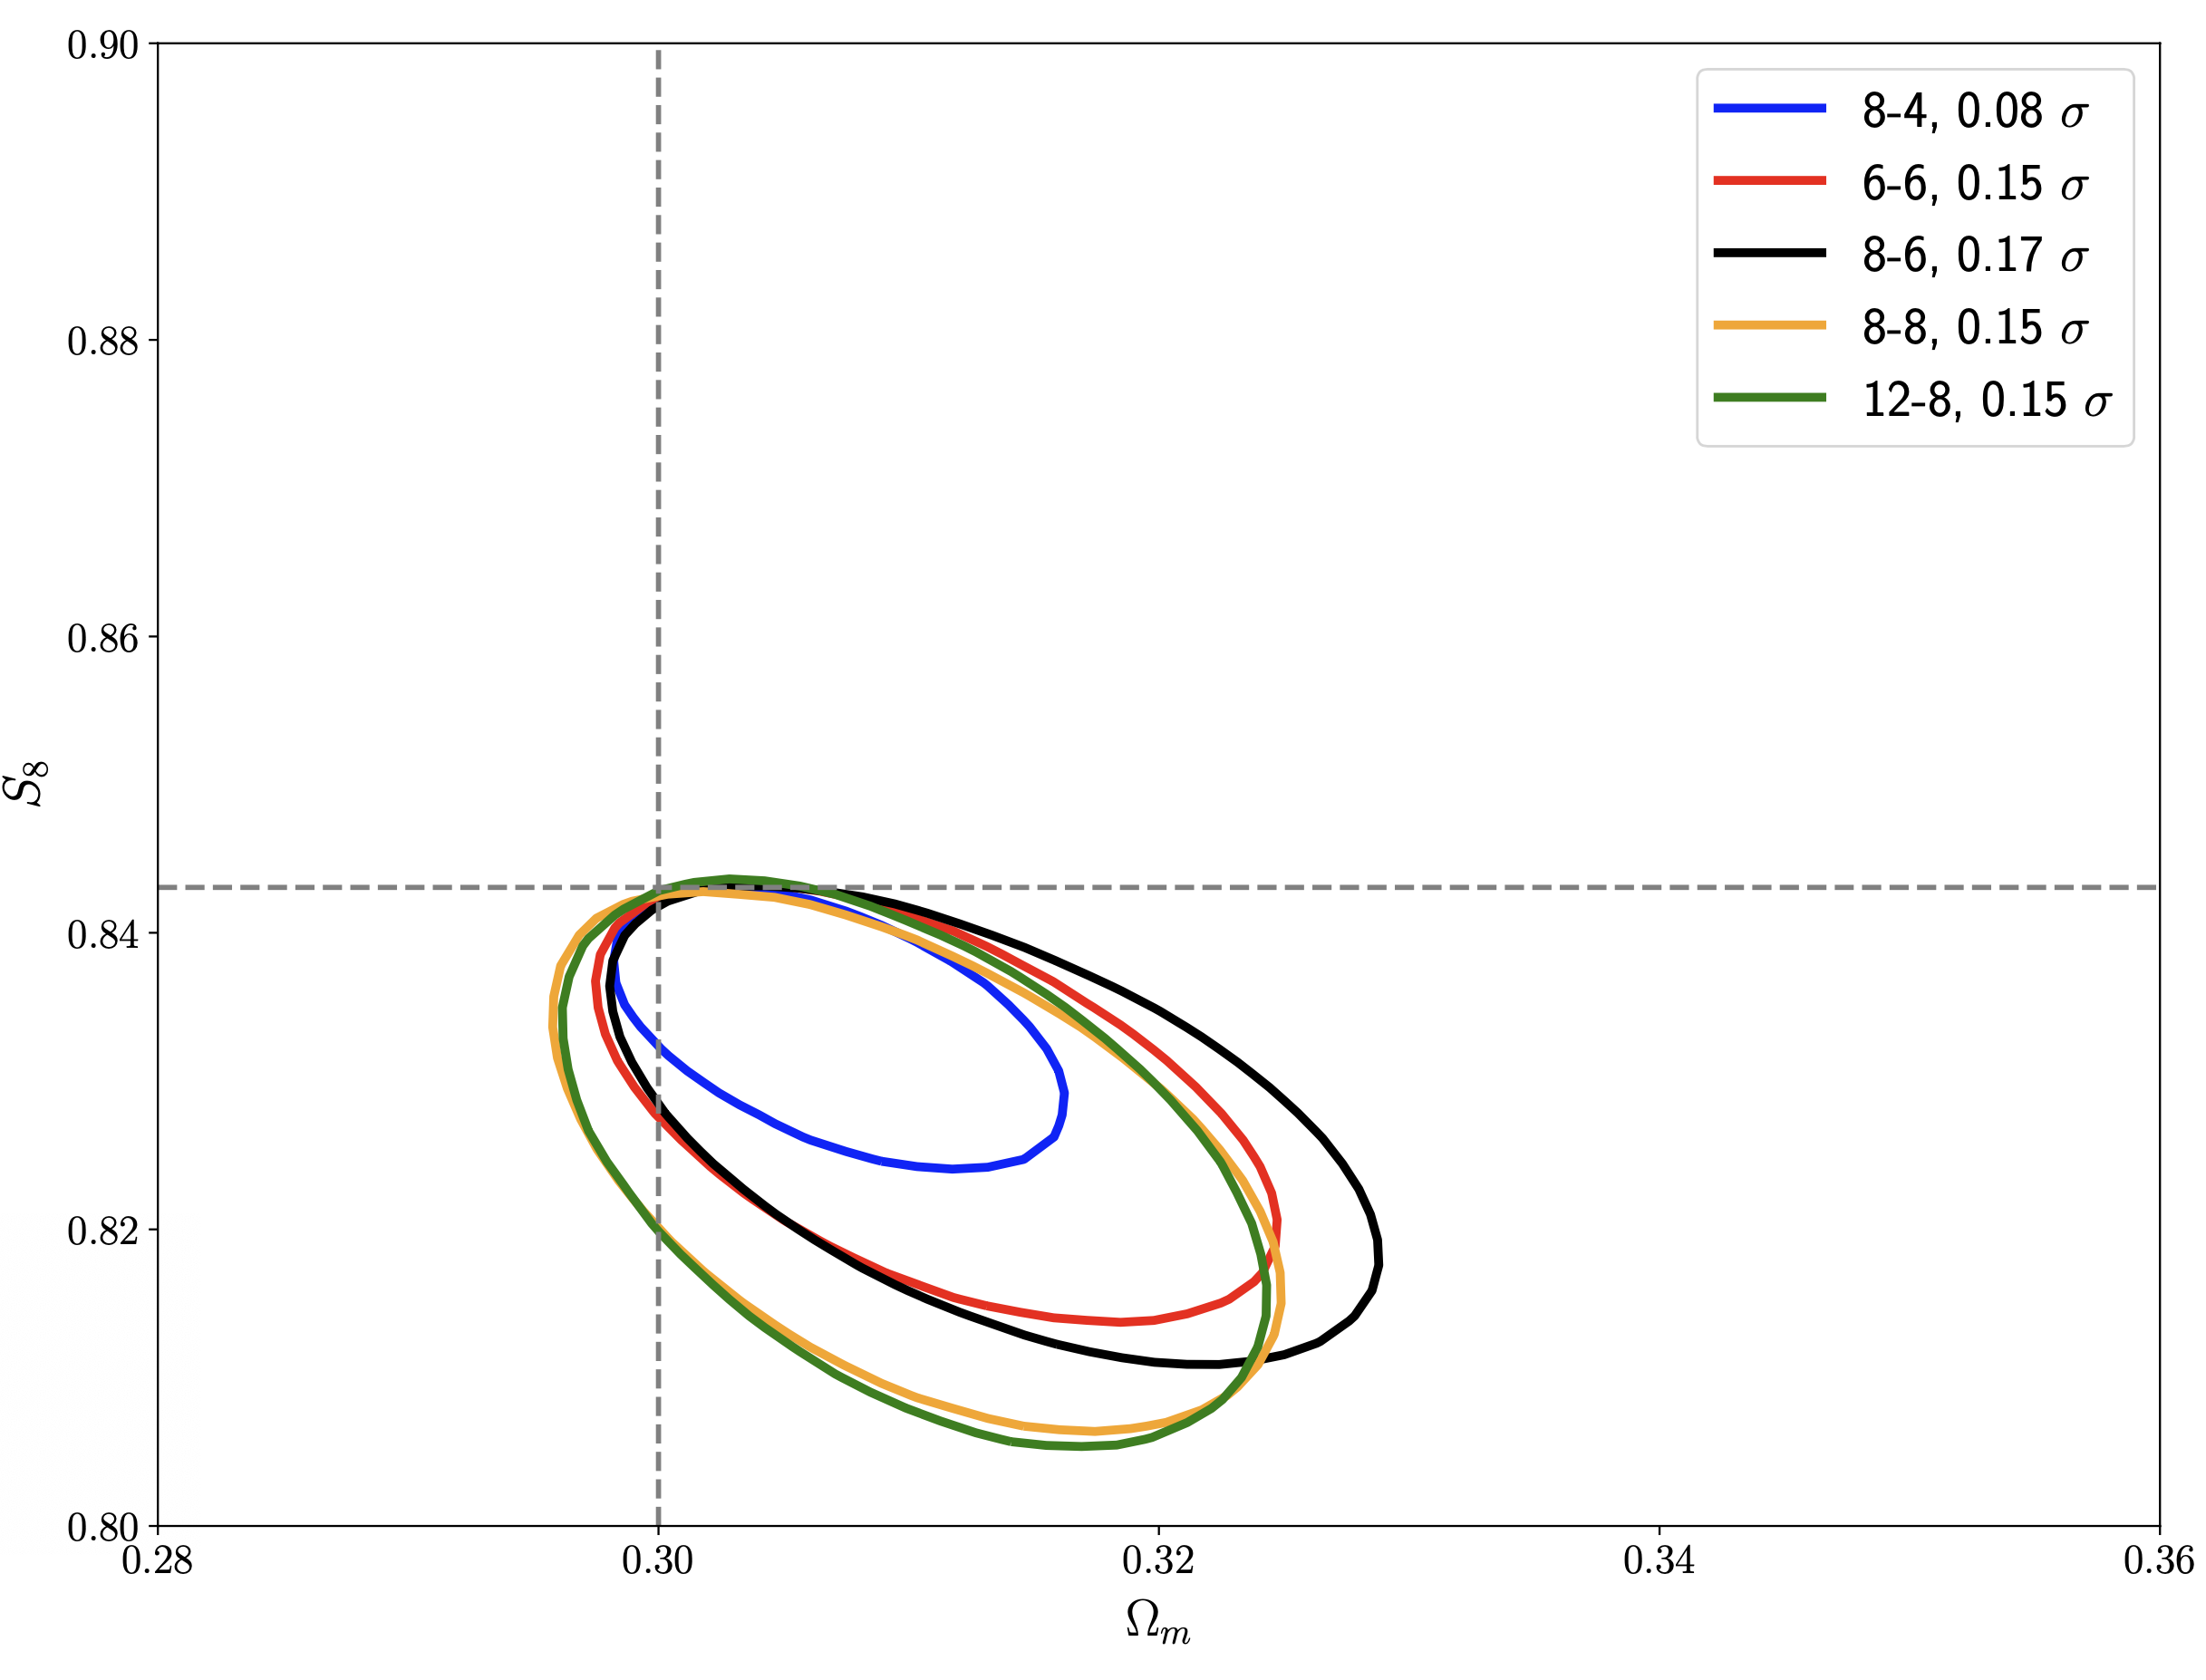
\includegraphics[width=\columnwidth,draft]{figs/temp.png}
\caption[]{Show the recovered bias values and the estimate from expected halo bias convolved with measured HOD from either small scales gglensing or in MICE. }
\label{fig:bias_relation}
\end{figure}

\section{Conclusions}




\section*{Acknowledgements}

The Acknowledgements section is not numbered. Here you can thank helpful
colleagues, acknowledge funding agencies, telescopes and facilities used etc.
Try to keep it short.

%%%%%%%%%%%%%%%%%%%%%%%%%%%%%%%%%%%%%%%%%%%%%%%%%%

%%%%%%%%%%%%%%%%%%%% REFERENCES %%%%%%%%%%%%%%%%%%

% The best way to enter references is to use BibTeX:

\bibliographystyle{mnras}
\bibliography{ref} % if your bibtex file is called example.bib


% Alternatively you could enter them by hand, like this:
% This method is tedious and prone to error if you have lots of references
% \begin{thebibliography}{99}
% \bibitem[\protect\citeauthoryear{Author}{2012}]{Author2012}
% Author A.~N., 2013, Journal of Improbable Astronomy, 1, 1
% \bibitem[\protect\citeauthoryear{Others}{2013}]{Others2013}
% Others S., 2012, Journal of Interesting Stuff, 17, 198
% \end{thebibliography}

%%%%%%%%%%%%%%%%%%%%%%%%%%%%%%%%%%%%%%%%%%%%%%%%%%

%%%%%%%%%%%%%%%%% APPENDICES %%%%%%%%%%%%%%%%%%%%%

\appendix

\section{Internal Consistency tests}

We use posterior predictive distribution (PPD) to test for internal consistency of the 2x2pt dataset. We test for the differences when removing selective tomograhic redshift bins and angular scales.

\red{Describe the PPD methodology}

\red{Describe that we also look at the posterior differences when the deviation from PPD is large}

\subsection{Tomographic Bins}

\subsection{Angular scales}


% \section{2$\times$2pt Measurements}\label{app:2x2pt_measure}

\section{Point mass marginalization}


\begin{figure}
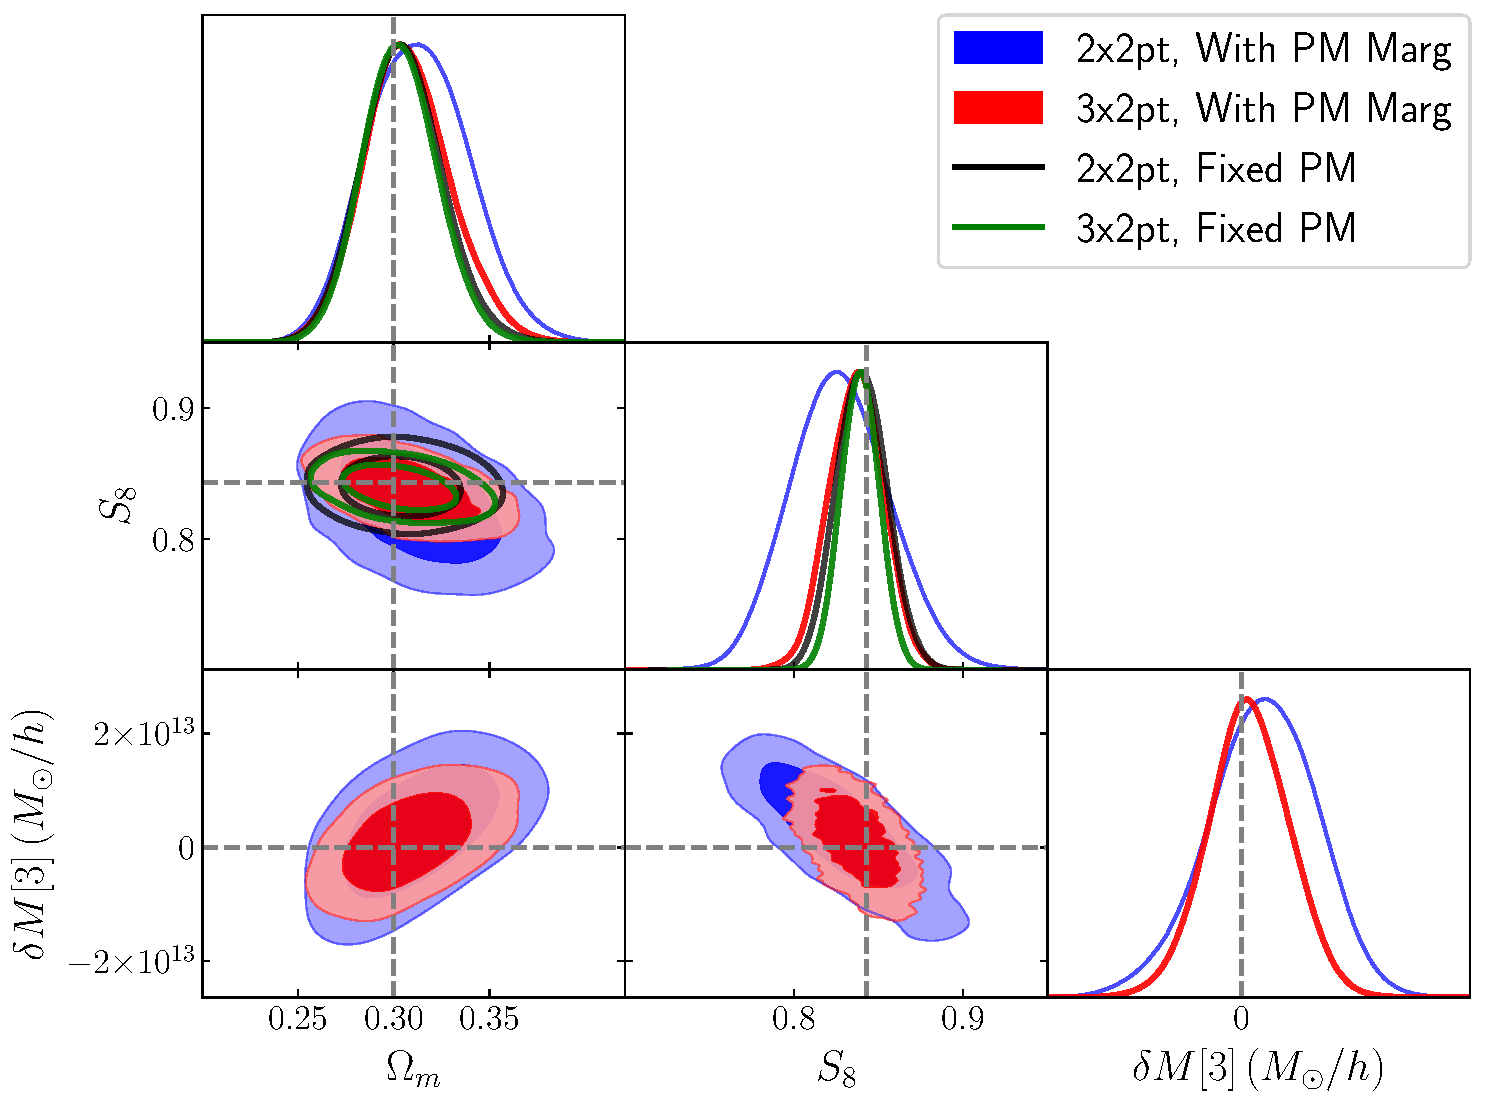
\includegraphics[width=\columnwidth]{figs/PM_constraints_2x2pt_3x2pt.pdf}
\caption[]{Effect of point mass marginalization on the constraining power of 2x2pt and 3x2pt. We see that the constraining power of 2x2pt degrades significantly with point mass marginalization, while for 3x2pt the change is minimal. Including the shear-shear correlation  breaks the degeneracy between point-mass (we show PM for third bin, $M_{\rm halo}[3]$) and $S_8$, leading to smaller sensitivity of cosmology constraints on point mass constraints. \SP{update the plot with non-zero PM in DV, to show the biases as well} }
\label{fig:pm_effect}
\end{figure}

\begin{figure}
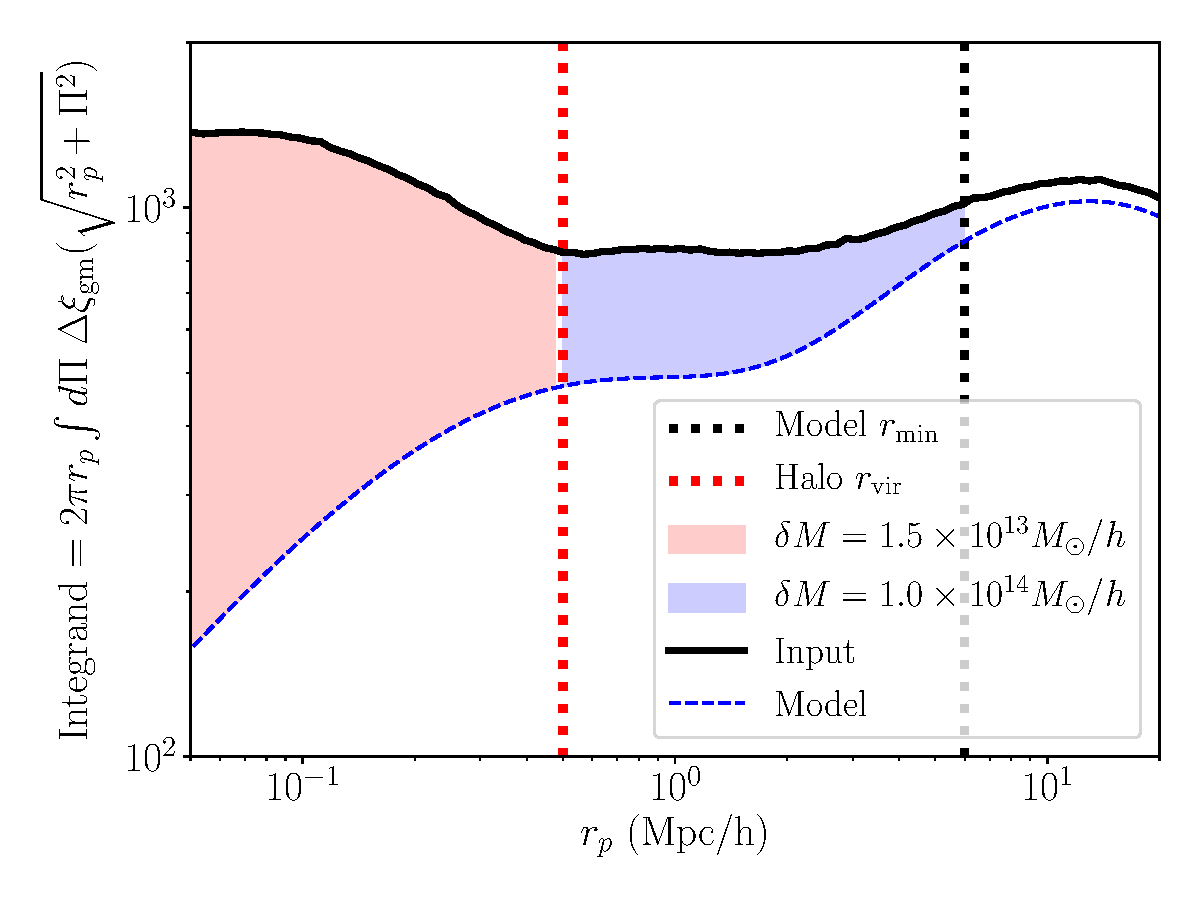
\includegraphics[width=\columnwidth]{figs/PM_contribution_radial.pdf}
\caption[]{We show the contribution of the PM to the galaxy-matter correlation in different radial regimes. The input is a halo-matter correlation function generated for a halo mass of $2.5 \times 10^{13} M_{\odot}/h$ using the NFW profile in the 1-halo regime ($r < 0.5 Mpc/h$) and 1Loop PT in the 2-halo regime ($r > 0.5 Mpc/h$). The model curve is generated from parameters within 1$\sigma$ of the truth. We show the contribution of the PM term separately for the 1-halo  and 2-halo regimes (up to the scale cut of 8Mpc/$h$). We find that the 2-halo regime contributes significantly. Therefore to put informative prior on the PM, the exact dependence of PM on cosmology and bias has to be known. 
}
\label{fig:pm_prior}
\end{figure}




\subsection{Model stress test}
\subsubsection{Evolution of Point-mass parameters}
The baseline model parameterization assumes the point mass parameter to be constant within each tomographic bin. We test this assumption by estimating the contribution that evolution of the galaxy-matter correlation function will have on the point mass parameters. Using a similar procedure as shown in Fig.~\ref{fig:pm_prior}, we estimate the integrand ($\delta_{\rm ev} M^{j}_{\rm halo}$) between evolved galaxy-matter correlation functions at edges of each tomographic bin $j$. These measured $\delta_{\rm ev} M^{j}_{\rm halo}$ quantify the expected bias in PM parameters due to evolution of the galaxy-matter correlations. These biases in PM parameters can potentially result in biased cosmology if it is a significant fraction of uncertainty in PM parameters ($\delta M^{j}_{\rm halo}$) for each tomographic bin $j$ (see Fig.~\ref{fig:pm_effect} for third tomographic bin) at our scale cuts. We compare the $\delta_{\rm ev} M^{j}_{\rm halo}$ to $\delta M^{j}_{\rm halo}$ in Fig.~\ref{fig:pm_evolve}. We see that for 2x2pt, the uncertainty in PM parameters is significantly greater than the expected bias. For 3x2pt, this bias is a significant fraction of the uncertainty but that will not bias our cosmology inference because as we have seen from Fig.~\ref{fig:pm_effect}, using shear information breaks the degeneracy between PM parameters and cosmological parameters.


\begin{figure}
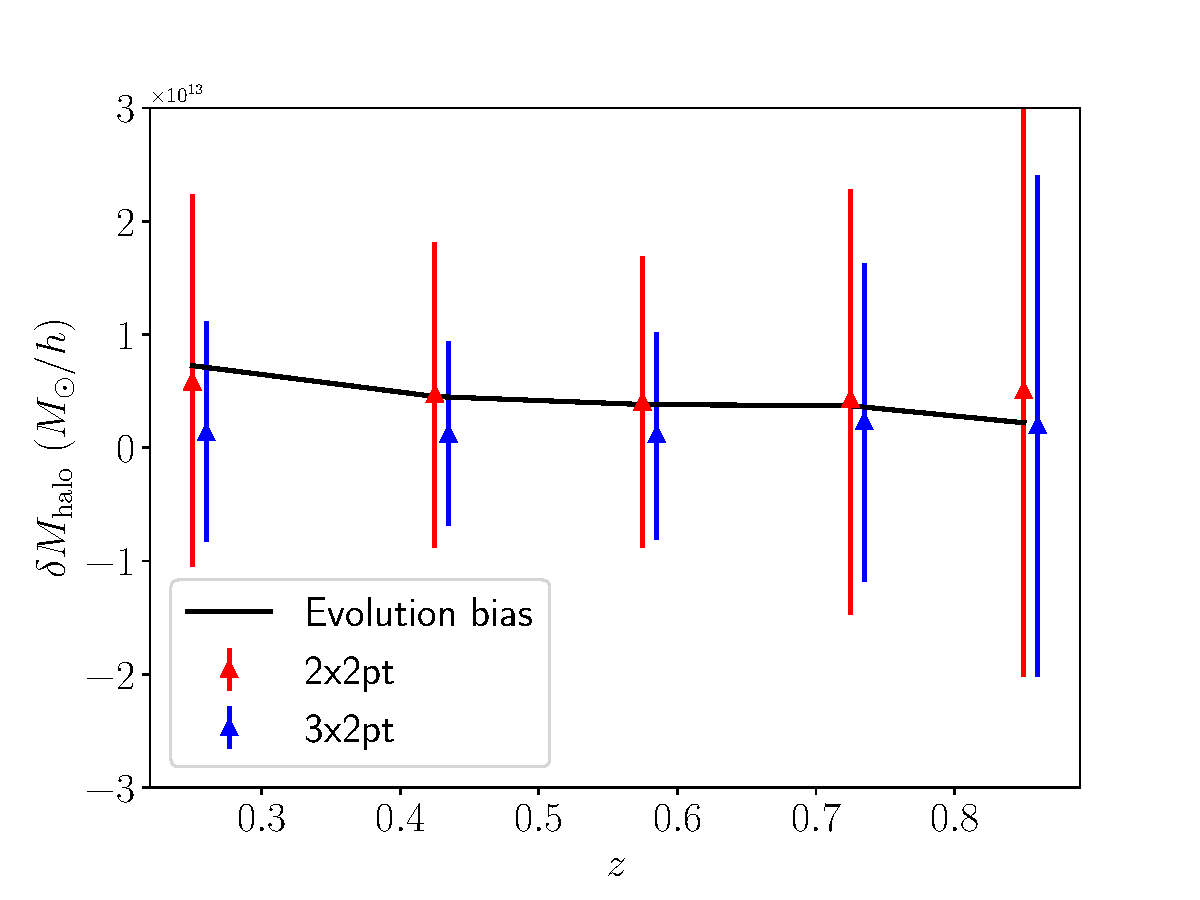
\includegraphics[width=\columnwidth]{figs/PM_evolve_impact.pdf}
\caption[]{We show the bias incurred from evolution of galaxy matter correlation on the PM parameters for each tomographic bin in black line. The red errorbars show the expected errorbars on PM parameters for 2x2pt as shown in Fig.~\ref{fig:pm_effect}. The blue errorbars are the constraints from 3x2pt. \SP{need to make this figure with non-zero PM values and at (8,6,0.5) scale cuts. It seems the impact will be even smaller there probably.}
}
\label{fig:pm_evolve}
\end{figure}

\subsubsection{Non-linear bias model assumptions}
\begin{figure}
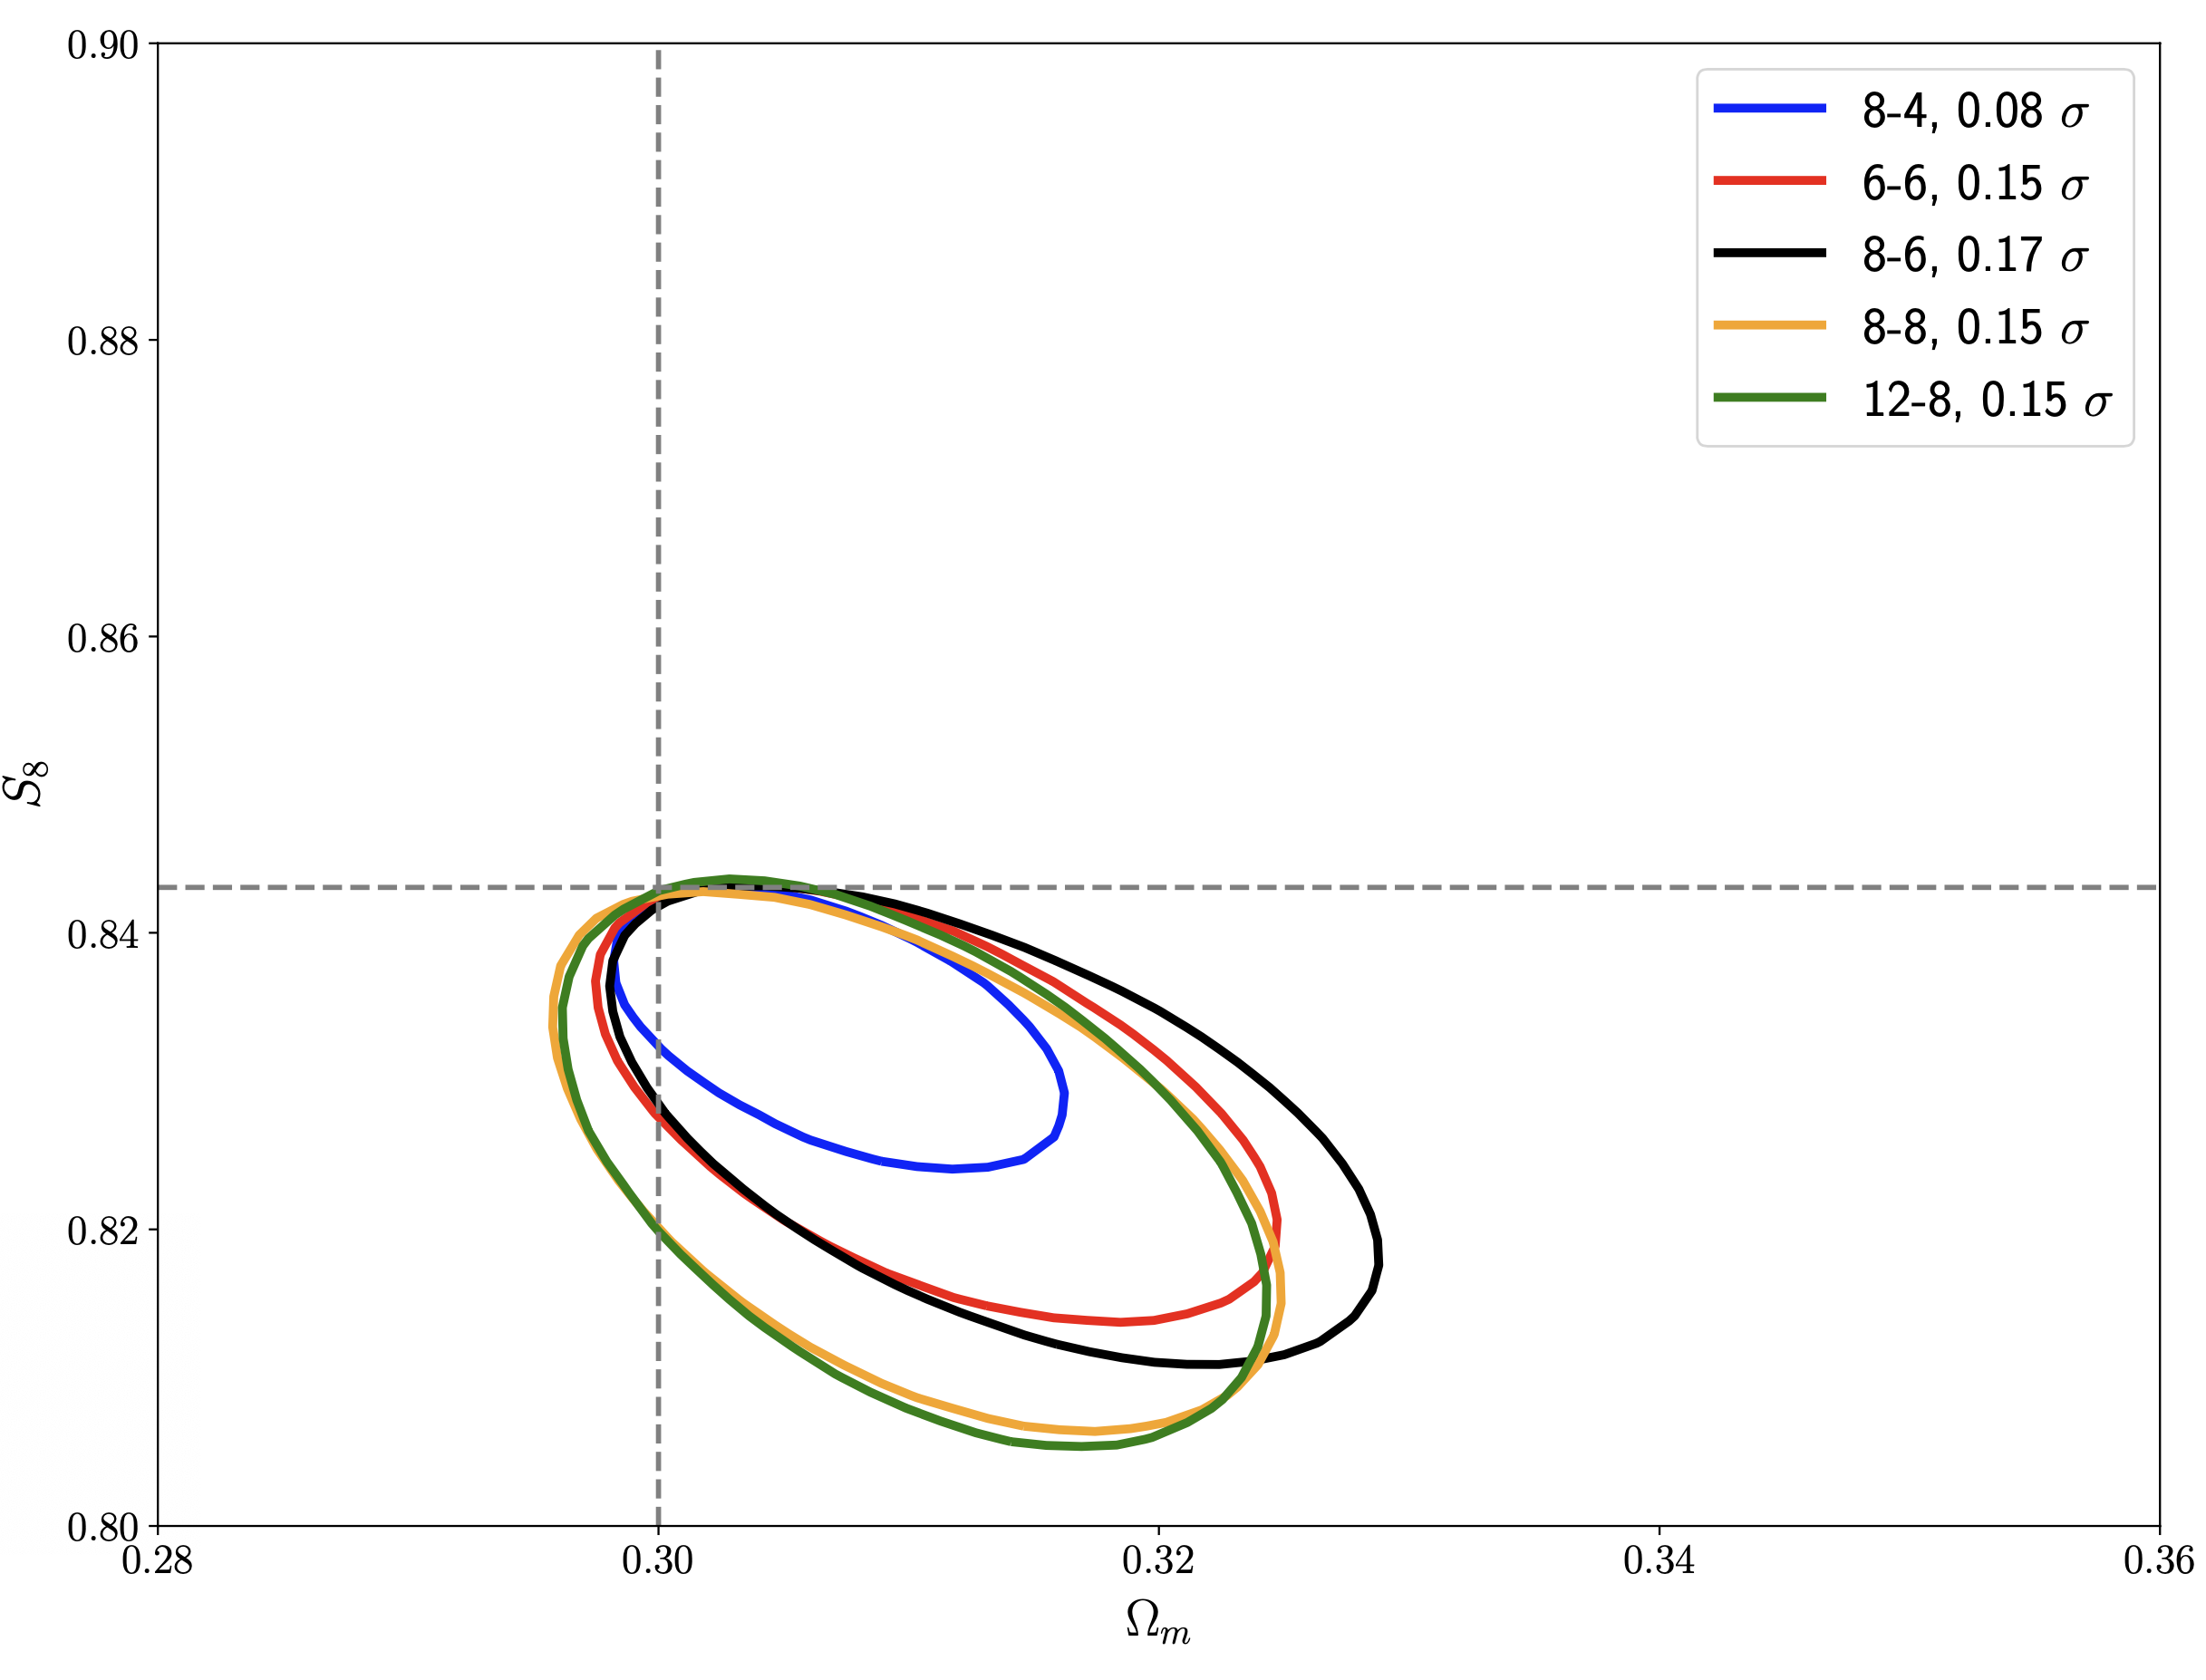
\includegraphics[width=0.48\textwidth,draft]{figs/temp.png}
\caption[]{Comparison of 1D or 2D $\Omega_m-S_8$ contours when analyzing with fiducial non-linear bias model ($b_s$ and $b_{\rm 3nl}$ fixed to co-evolution value) a datavector with $b_s$ and $b_{\rm 3nl}$ shifted by 1$\sigma$ (as given by 3D tests). This will validate our fiducial non-linear bias model from a simulated likelihood method. }
\label{fig:nlbias_bsb3nl}
\end{figure}

% \begin{figure}
% 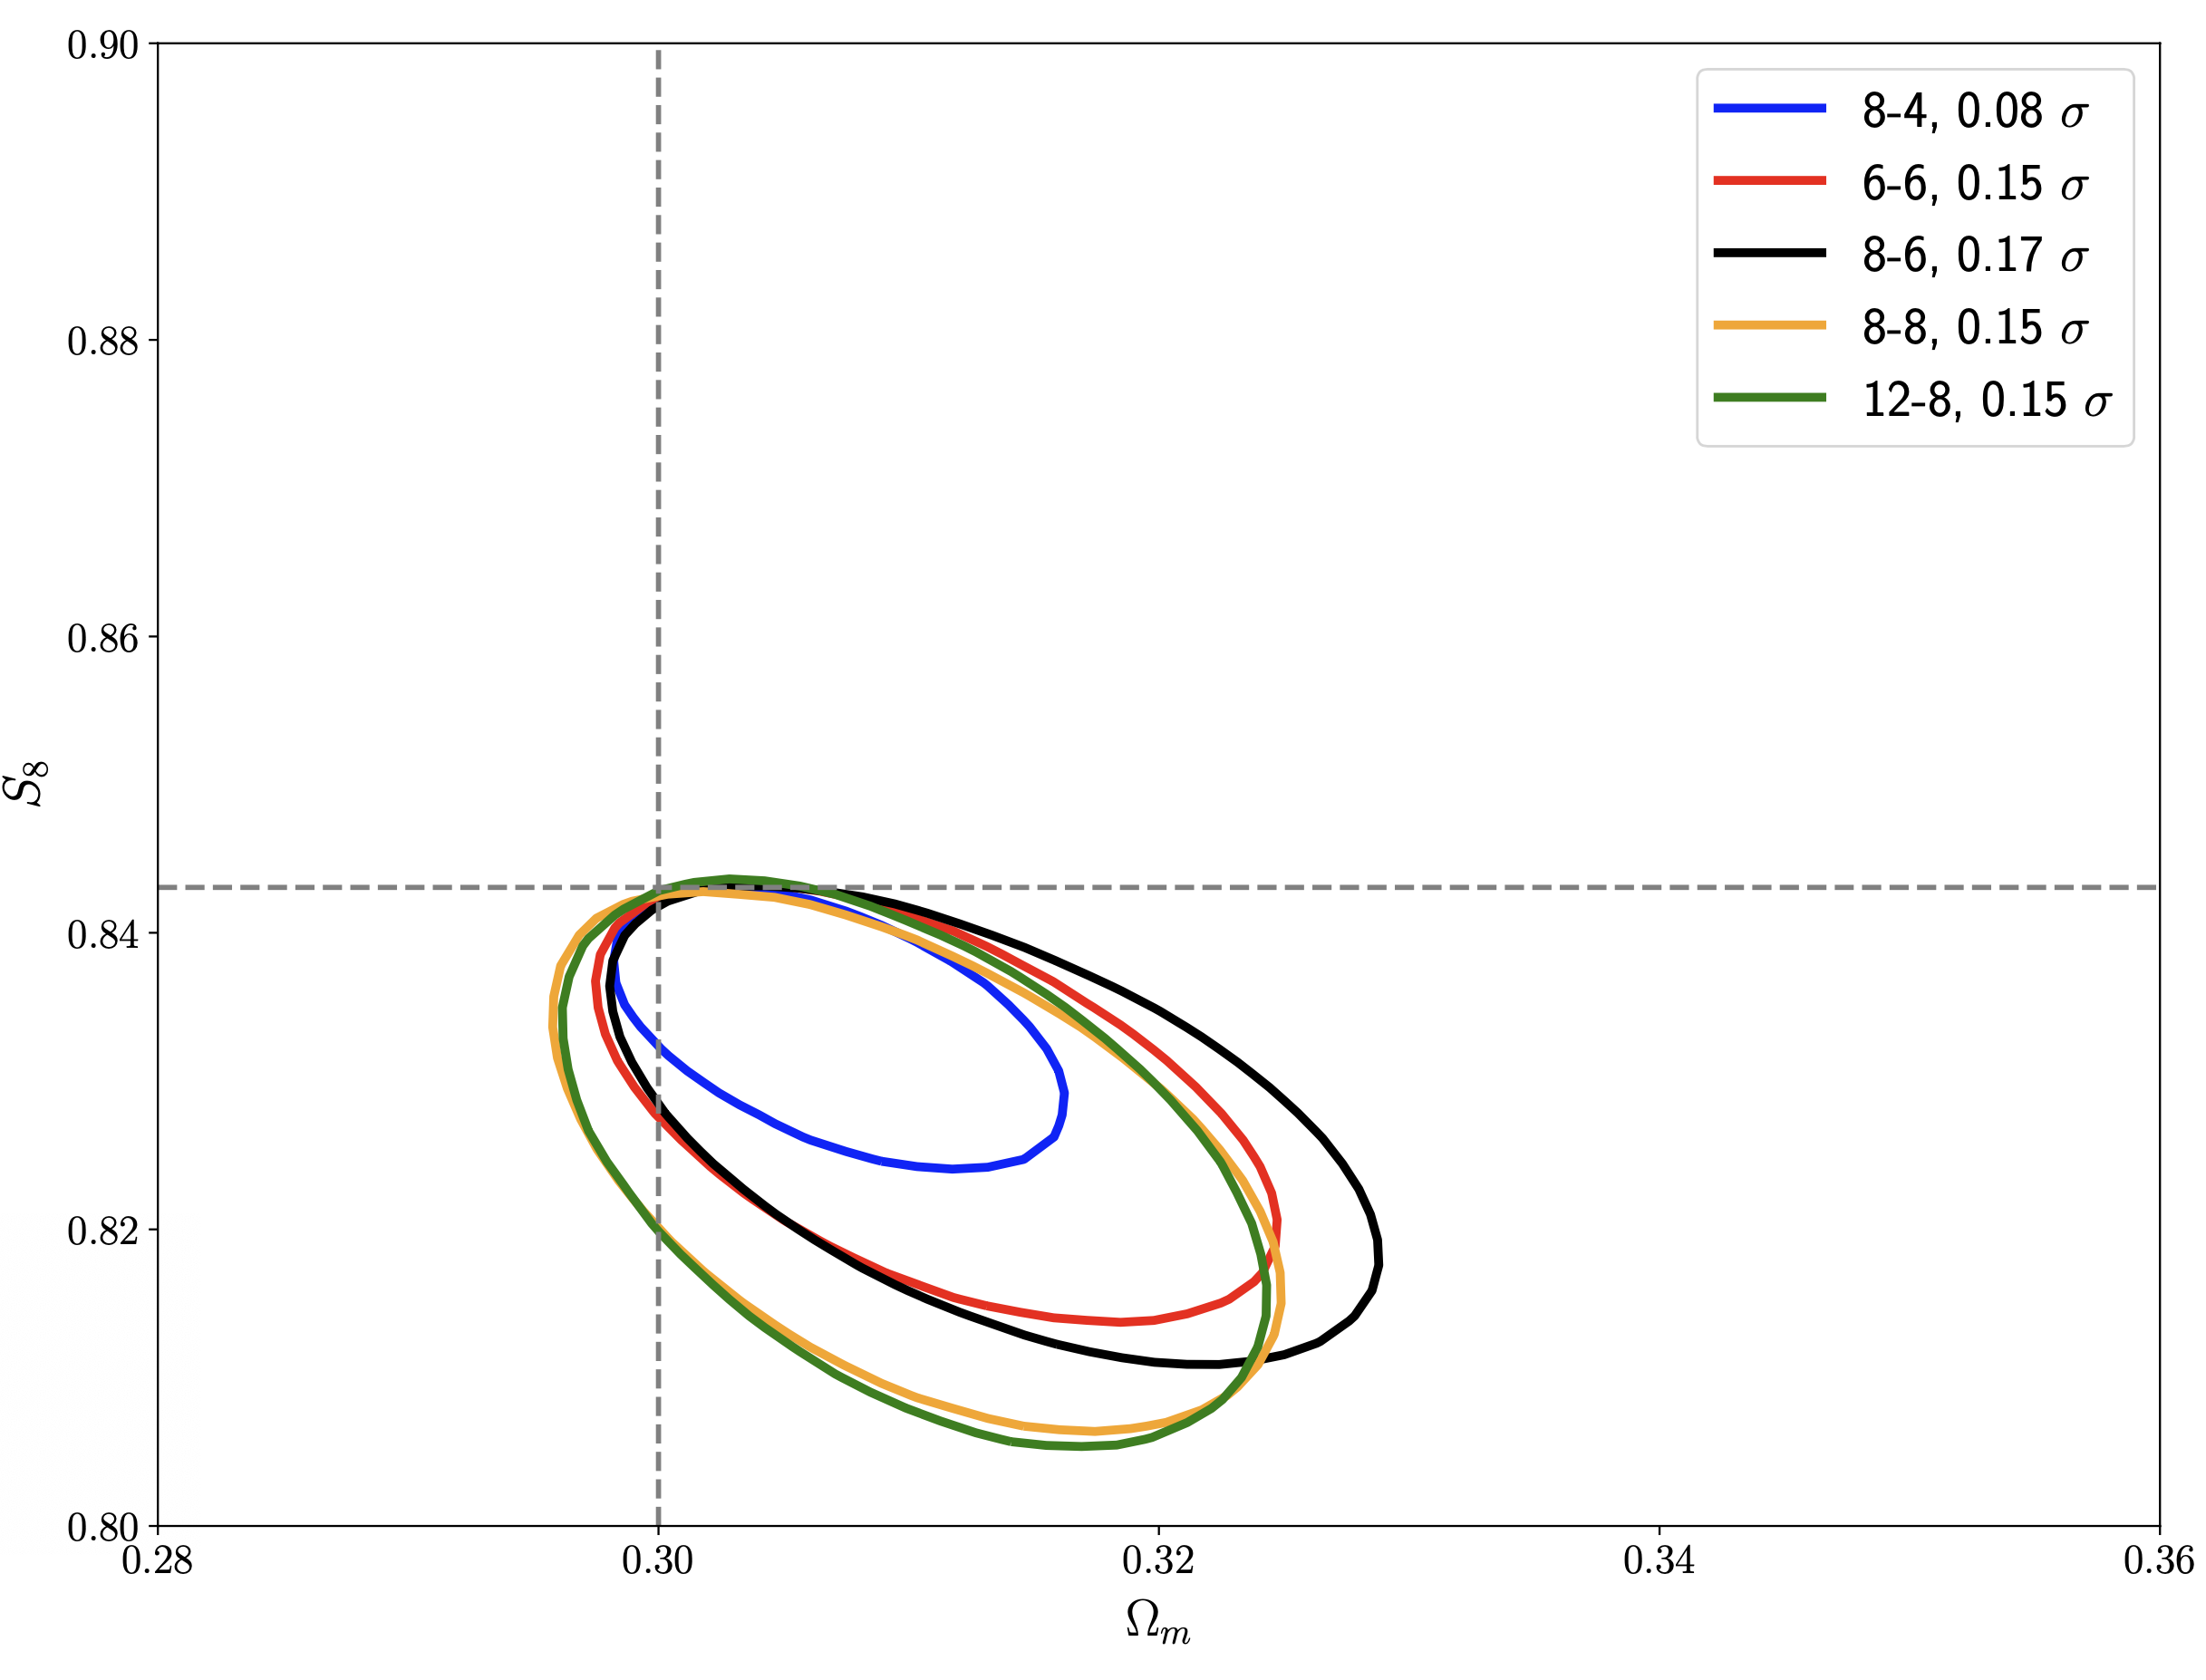
\includegraphics[width=0.5\textwidth,draft]{figs/temp.png}
% \caption[]{Show the contours when freeing up the $b_k$ parameters.}
% \label{fig:nlbias_bk}
% \end{figure}



\subsection{Simulations}

\begin{figure}
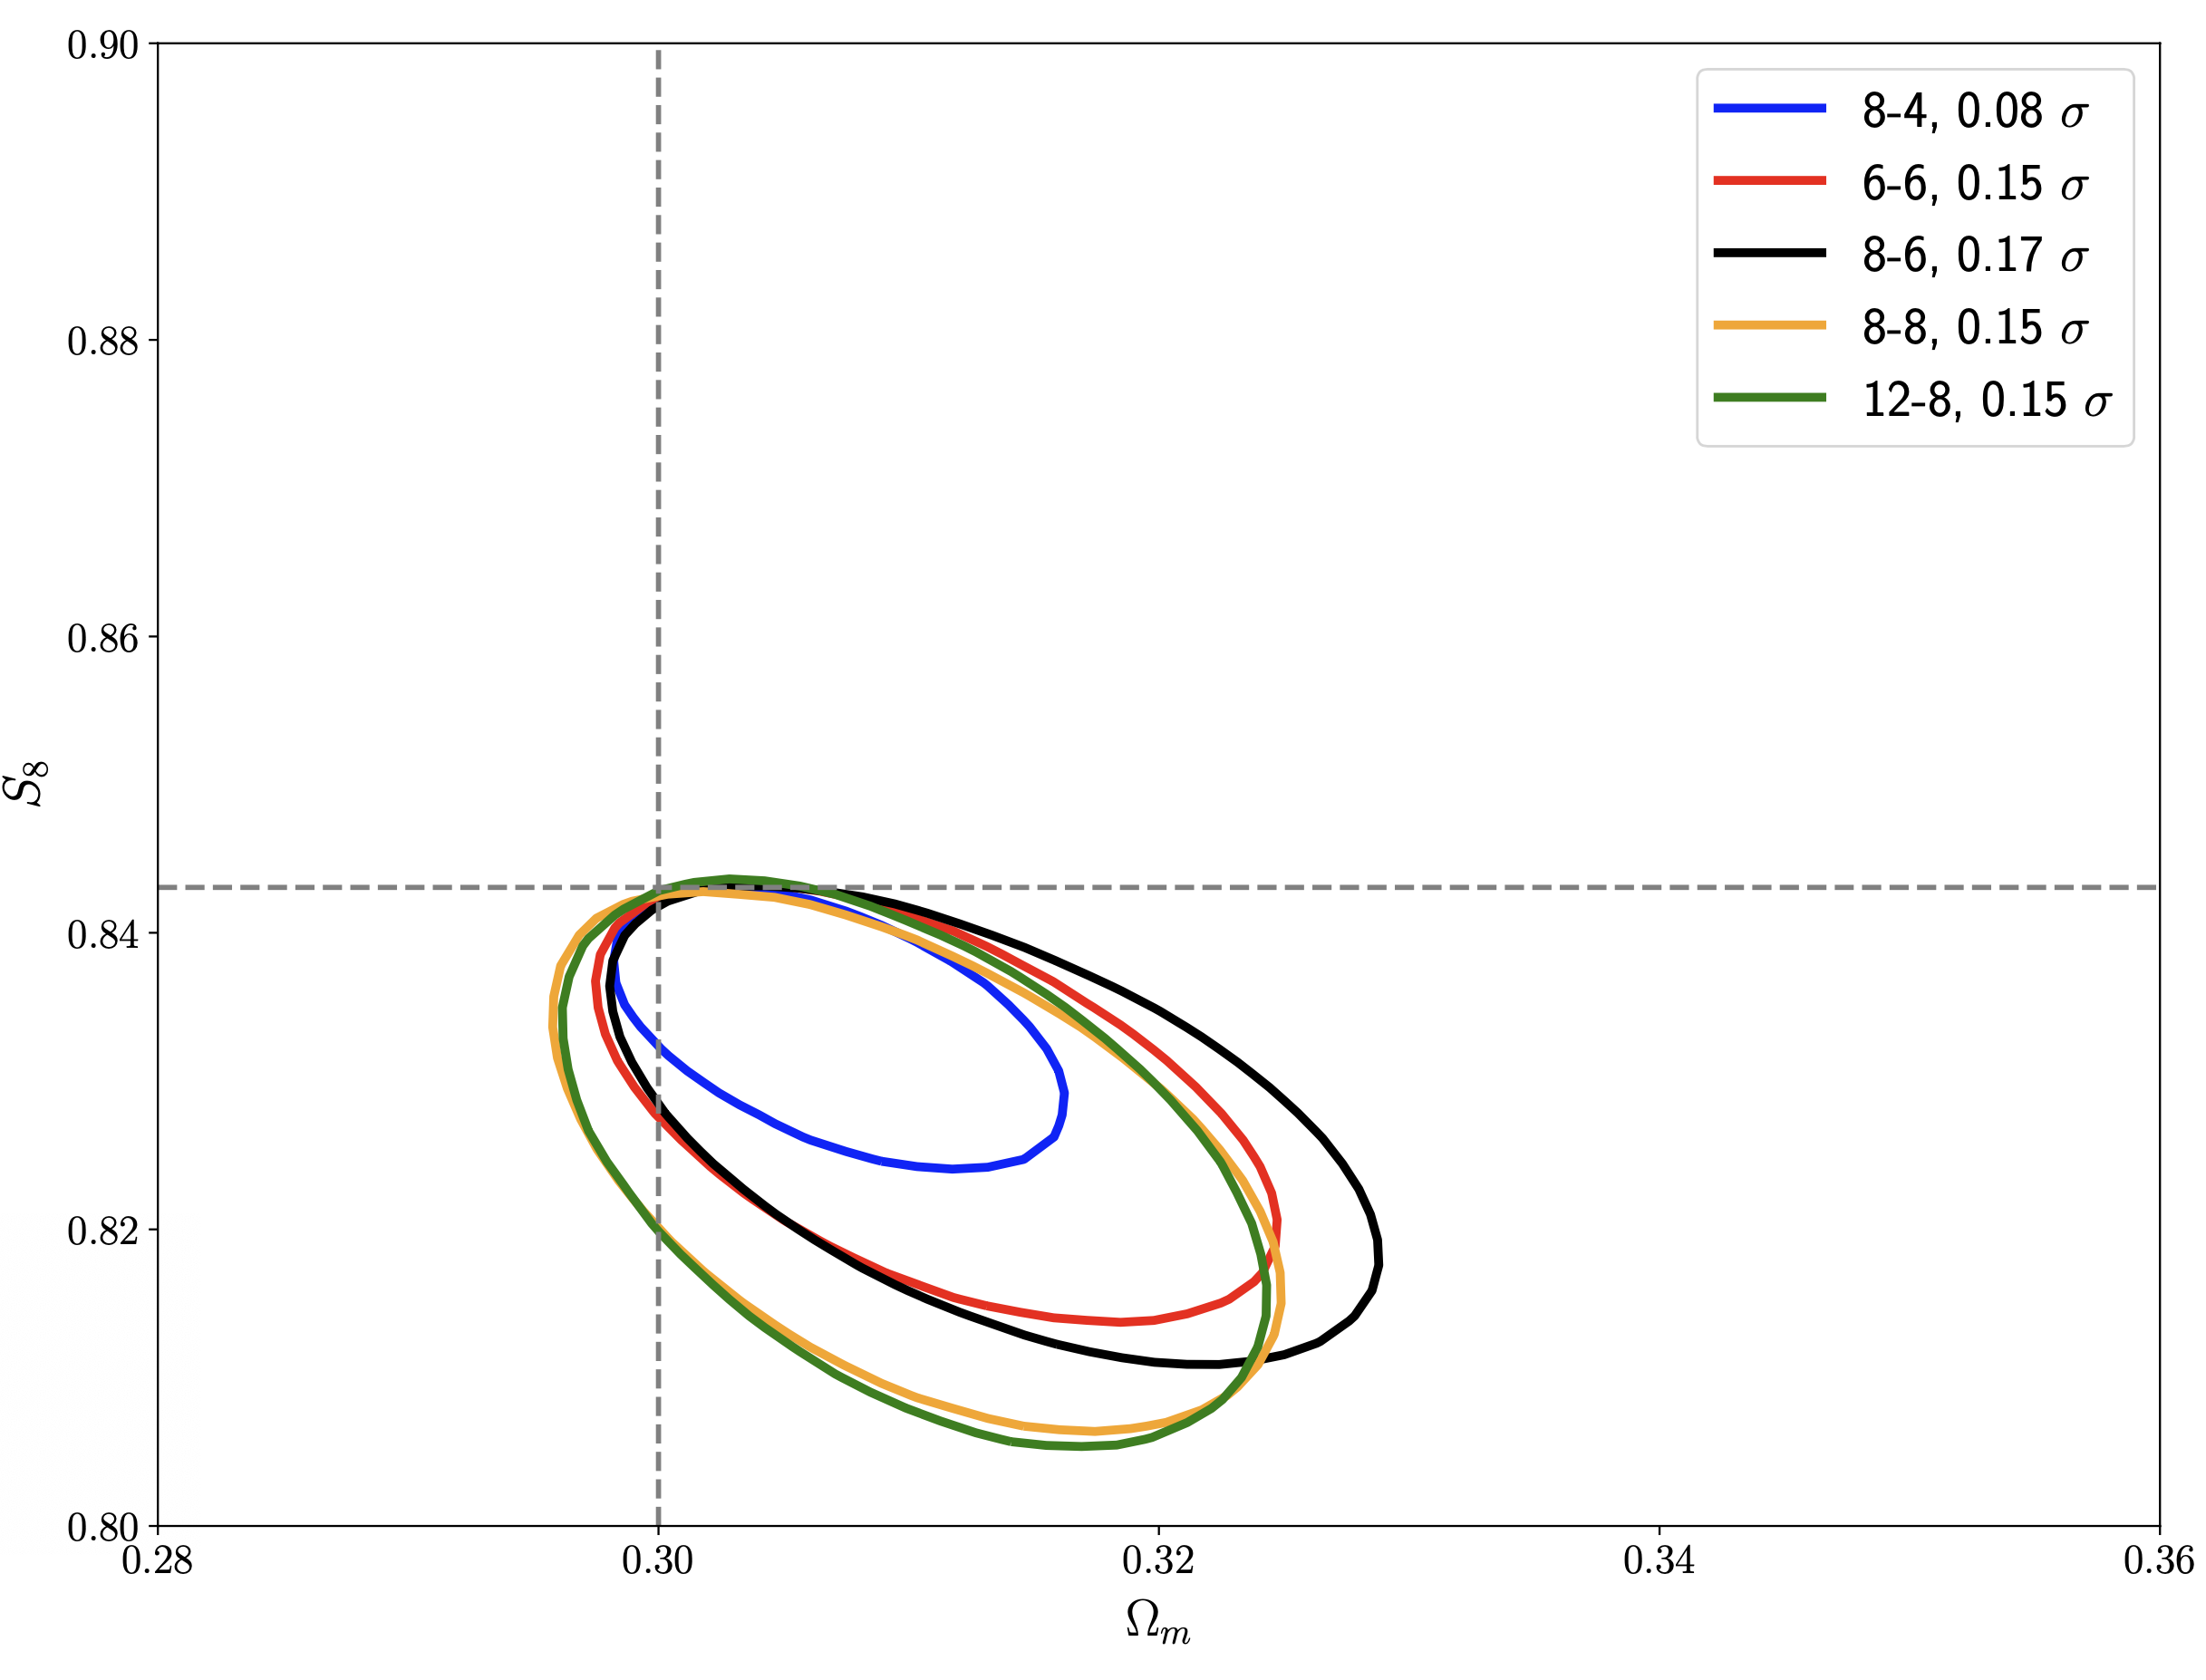
\includegraphics[width=0.5\textwidth,draft]{figs/temp.png}
\caption[]{Measurements and best-fit of \wtheta and \gammat for \buzzard \ simulations. 
% Show results for mean of N realizations and bestfit theory 
}
\label{fig:buzzard_2pt}
\end{figure}

\begin{figure}
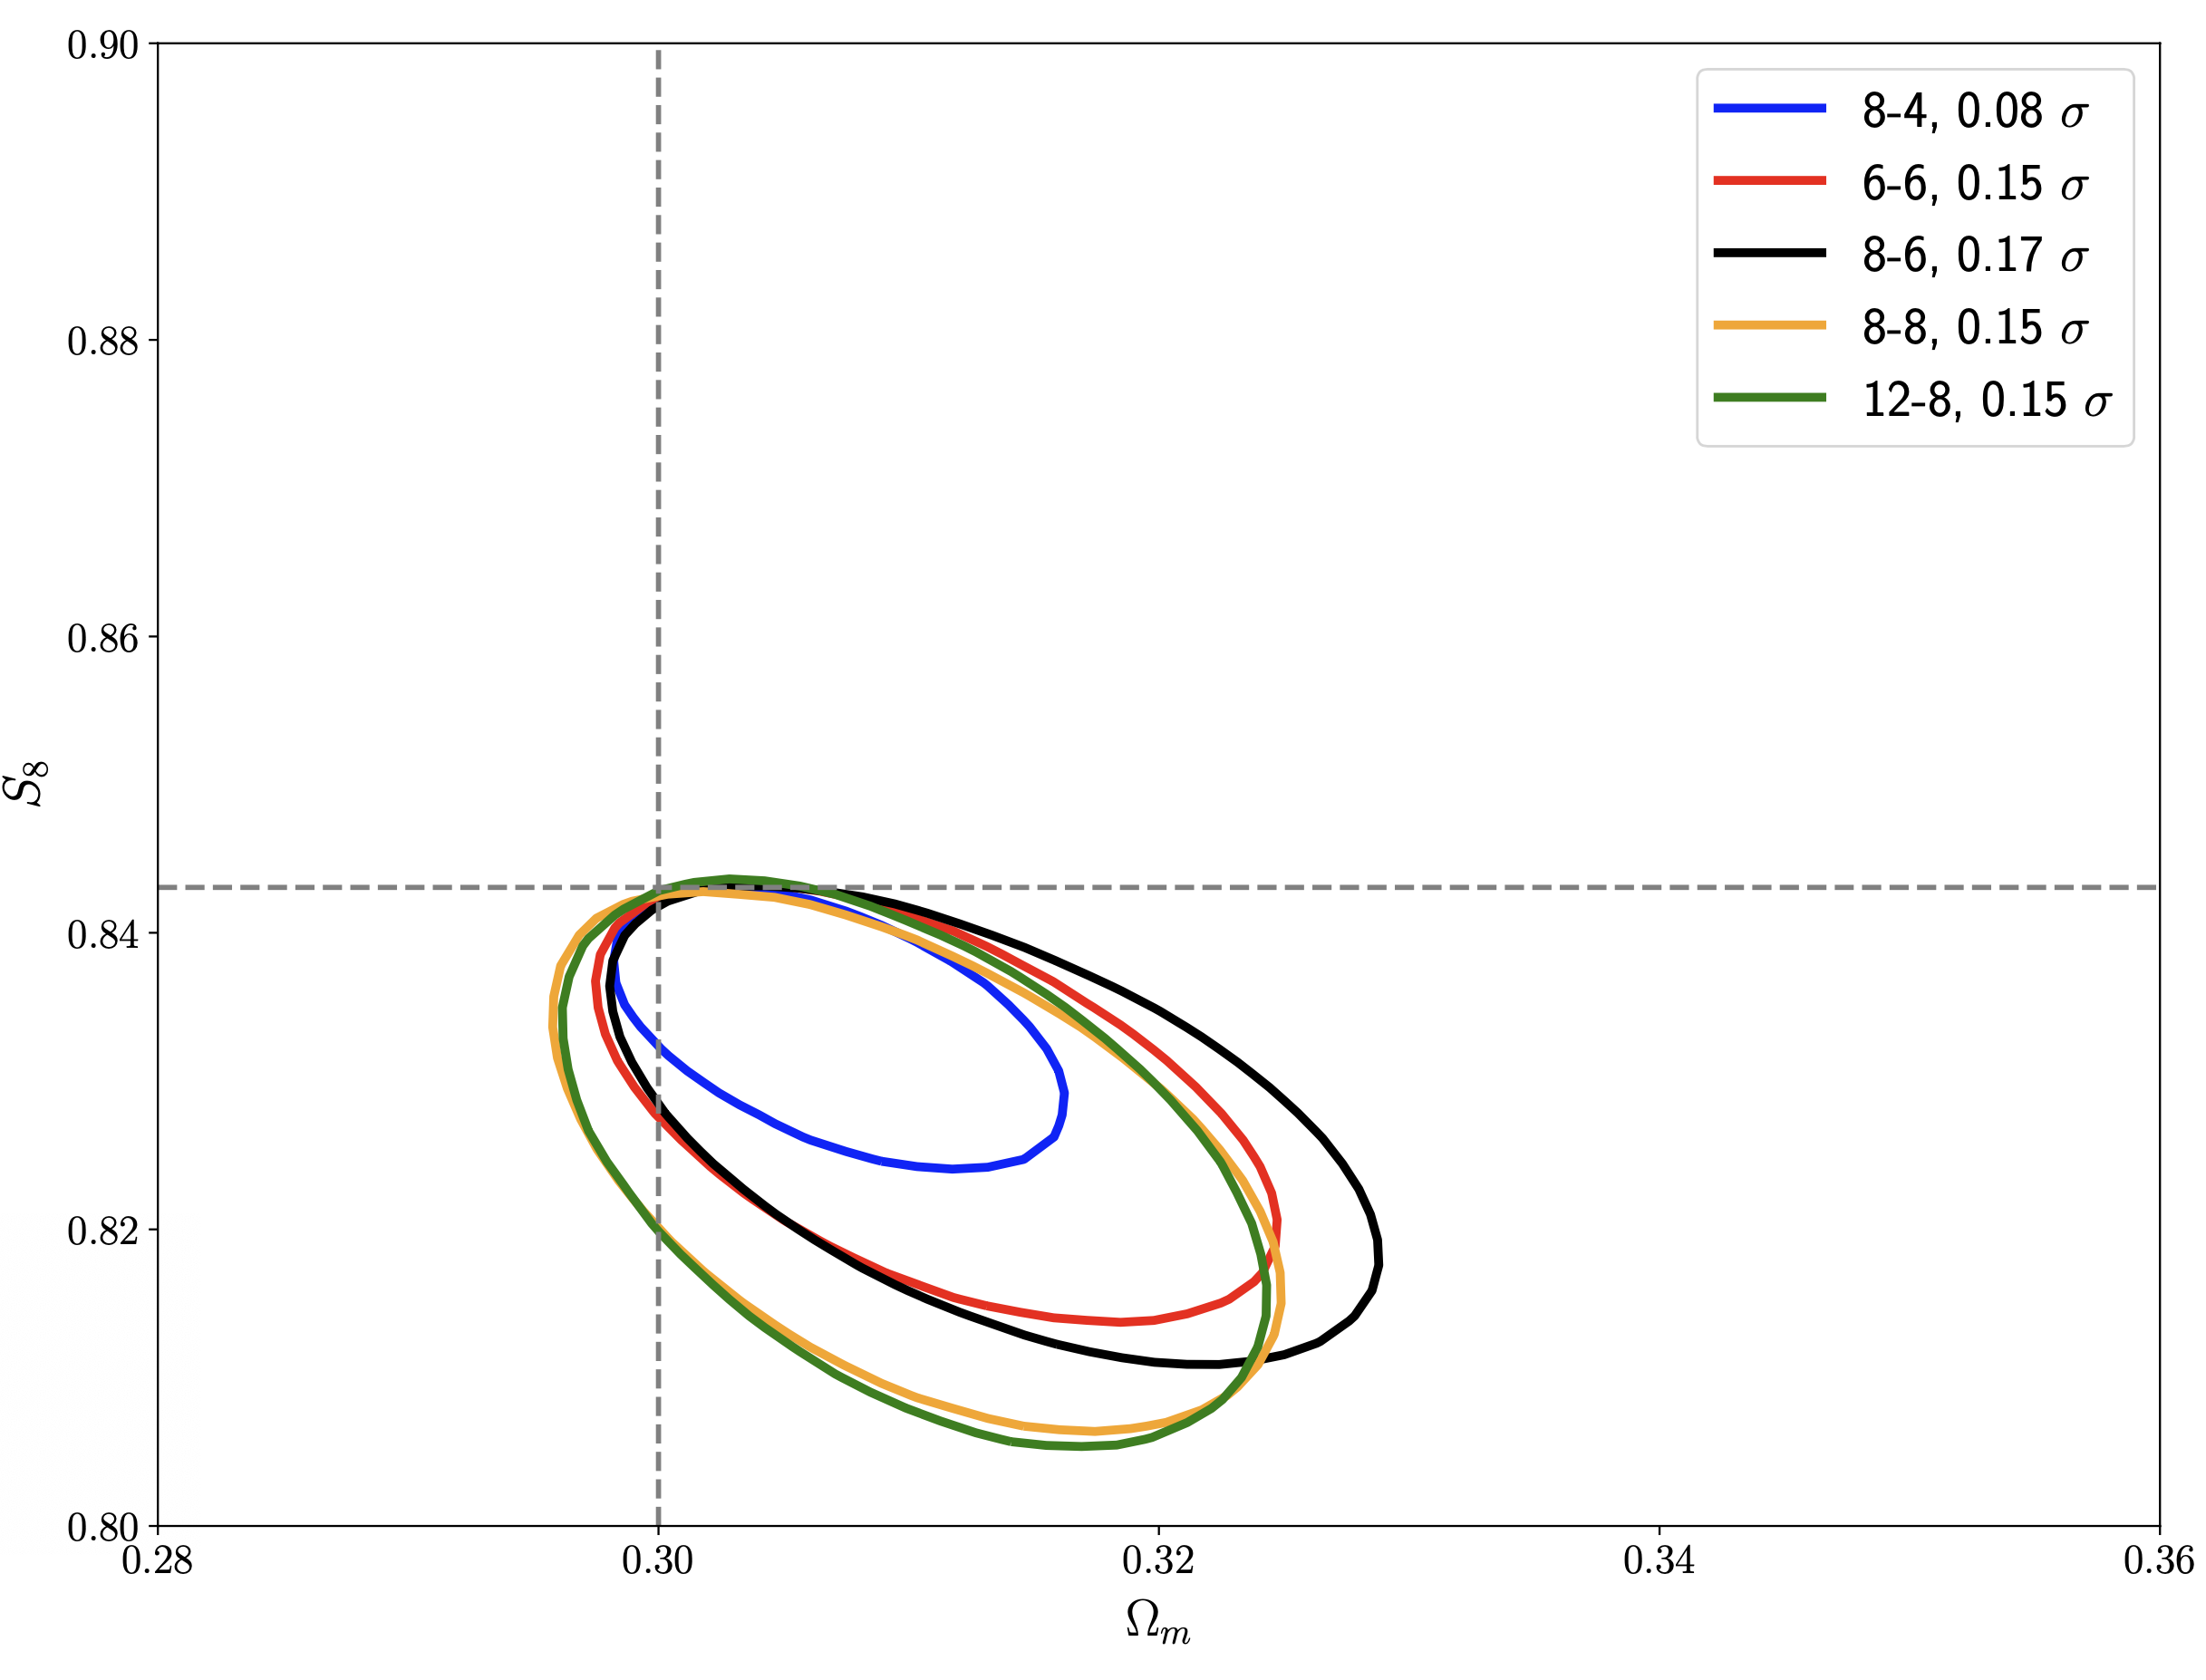
\includegraphics[width=0.5\textwidth,draft]{figs/temp.png}
\caption[]{Measurements and best-fit of \wtheta and \gammat for \mice \  simulations }
\label{fig:mice_2pt}
\end{figure}

\subsection{DES Y3}
\begin{figure}
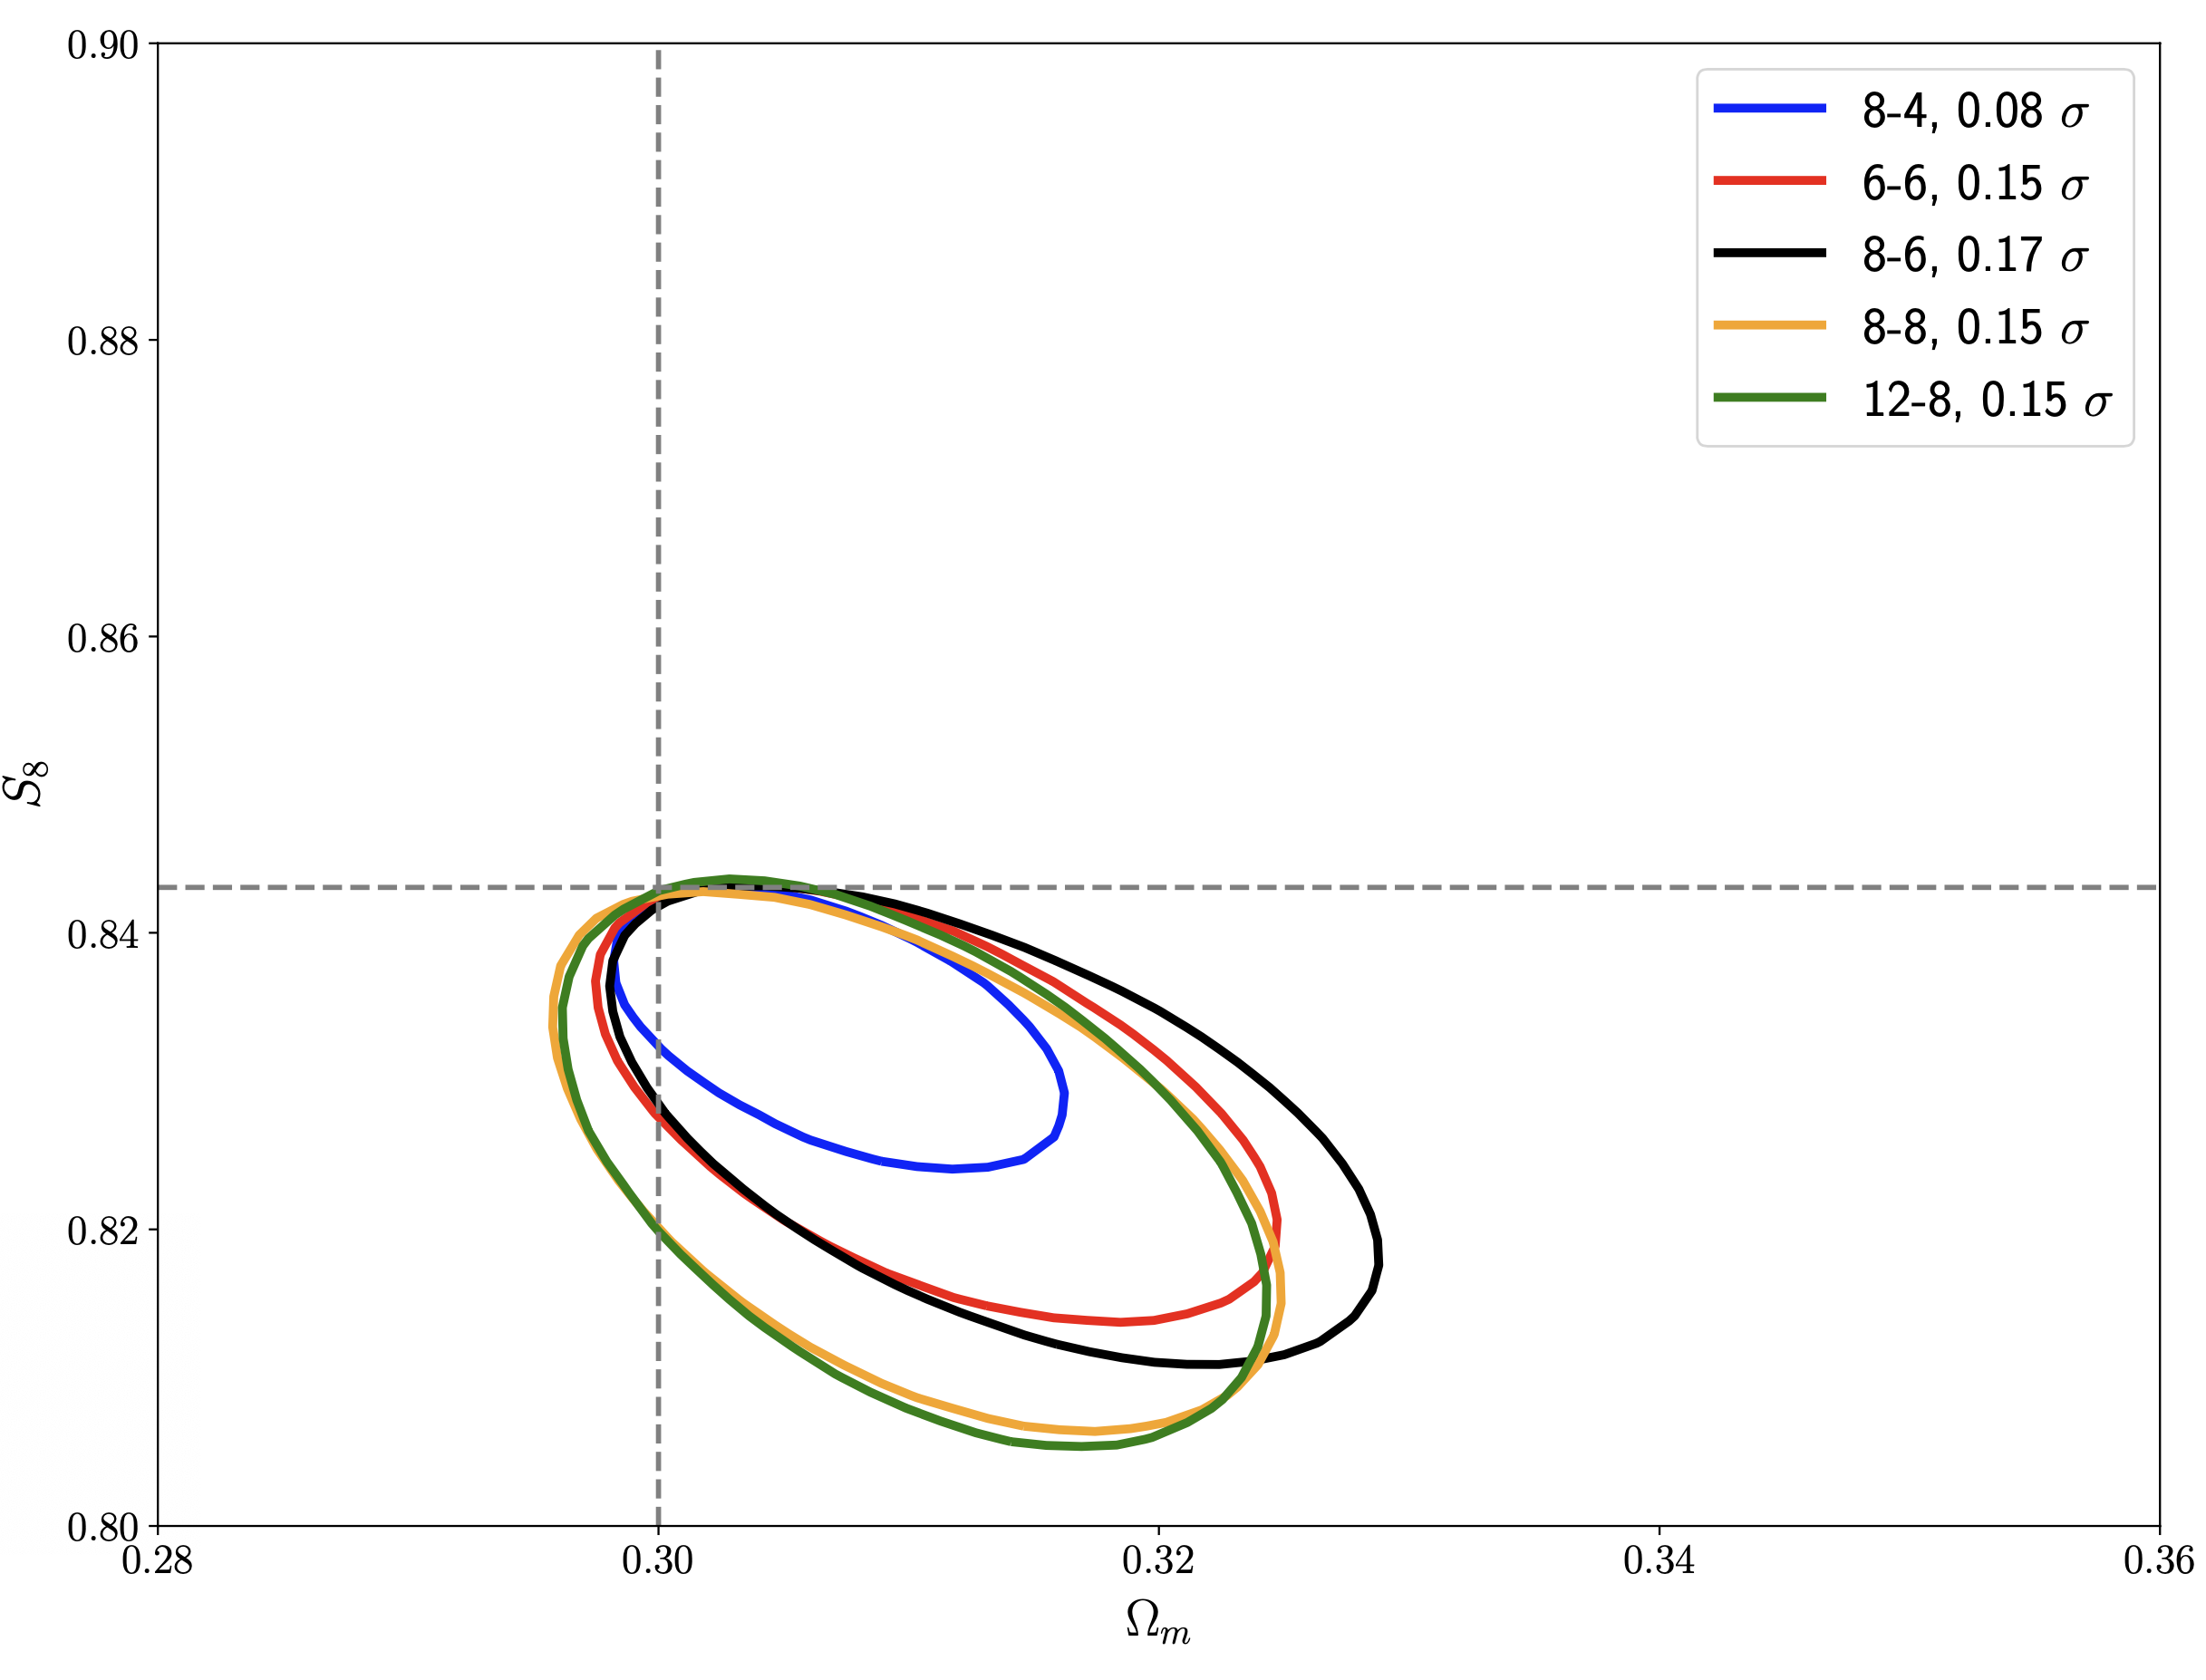
\includegraphics[width=0.5\textwidth,draft]{figs/temp.png}
\caption[]{Measurements and best-fit of $\wtheta$ and $\gammat$ with DES Y3 data }
\label{fig:data_2pt}
\end{figure}

\section{Scale cuts validation}\label{app:scale_cuts}
\subsection{Projection effects}\label{app:projection_effects}

% \begin{figure}
% 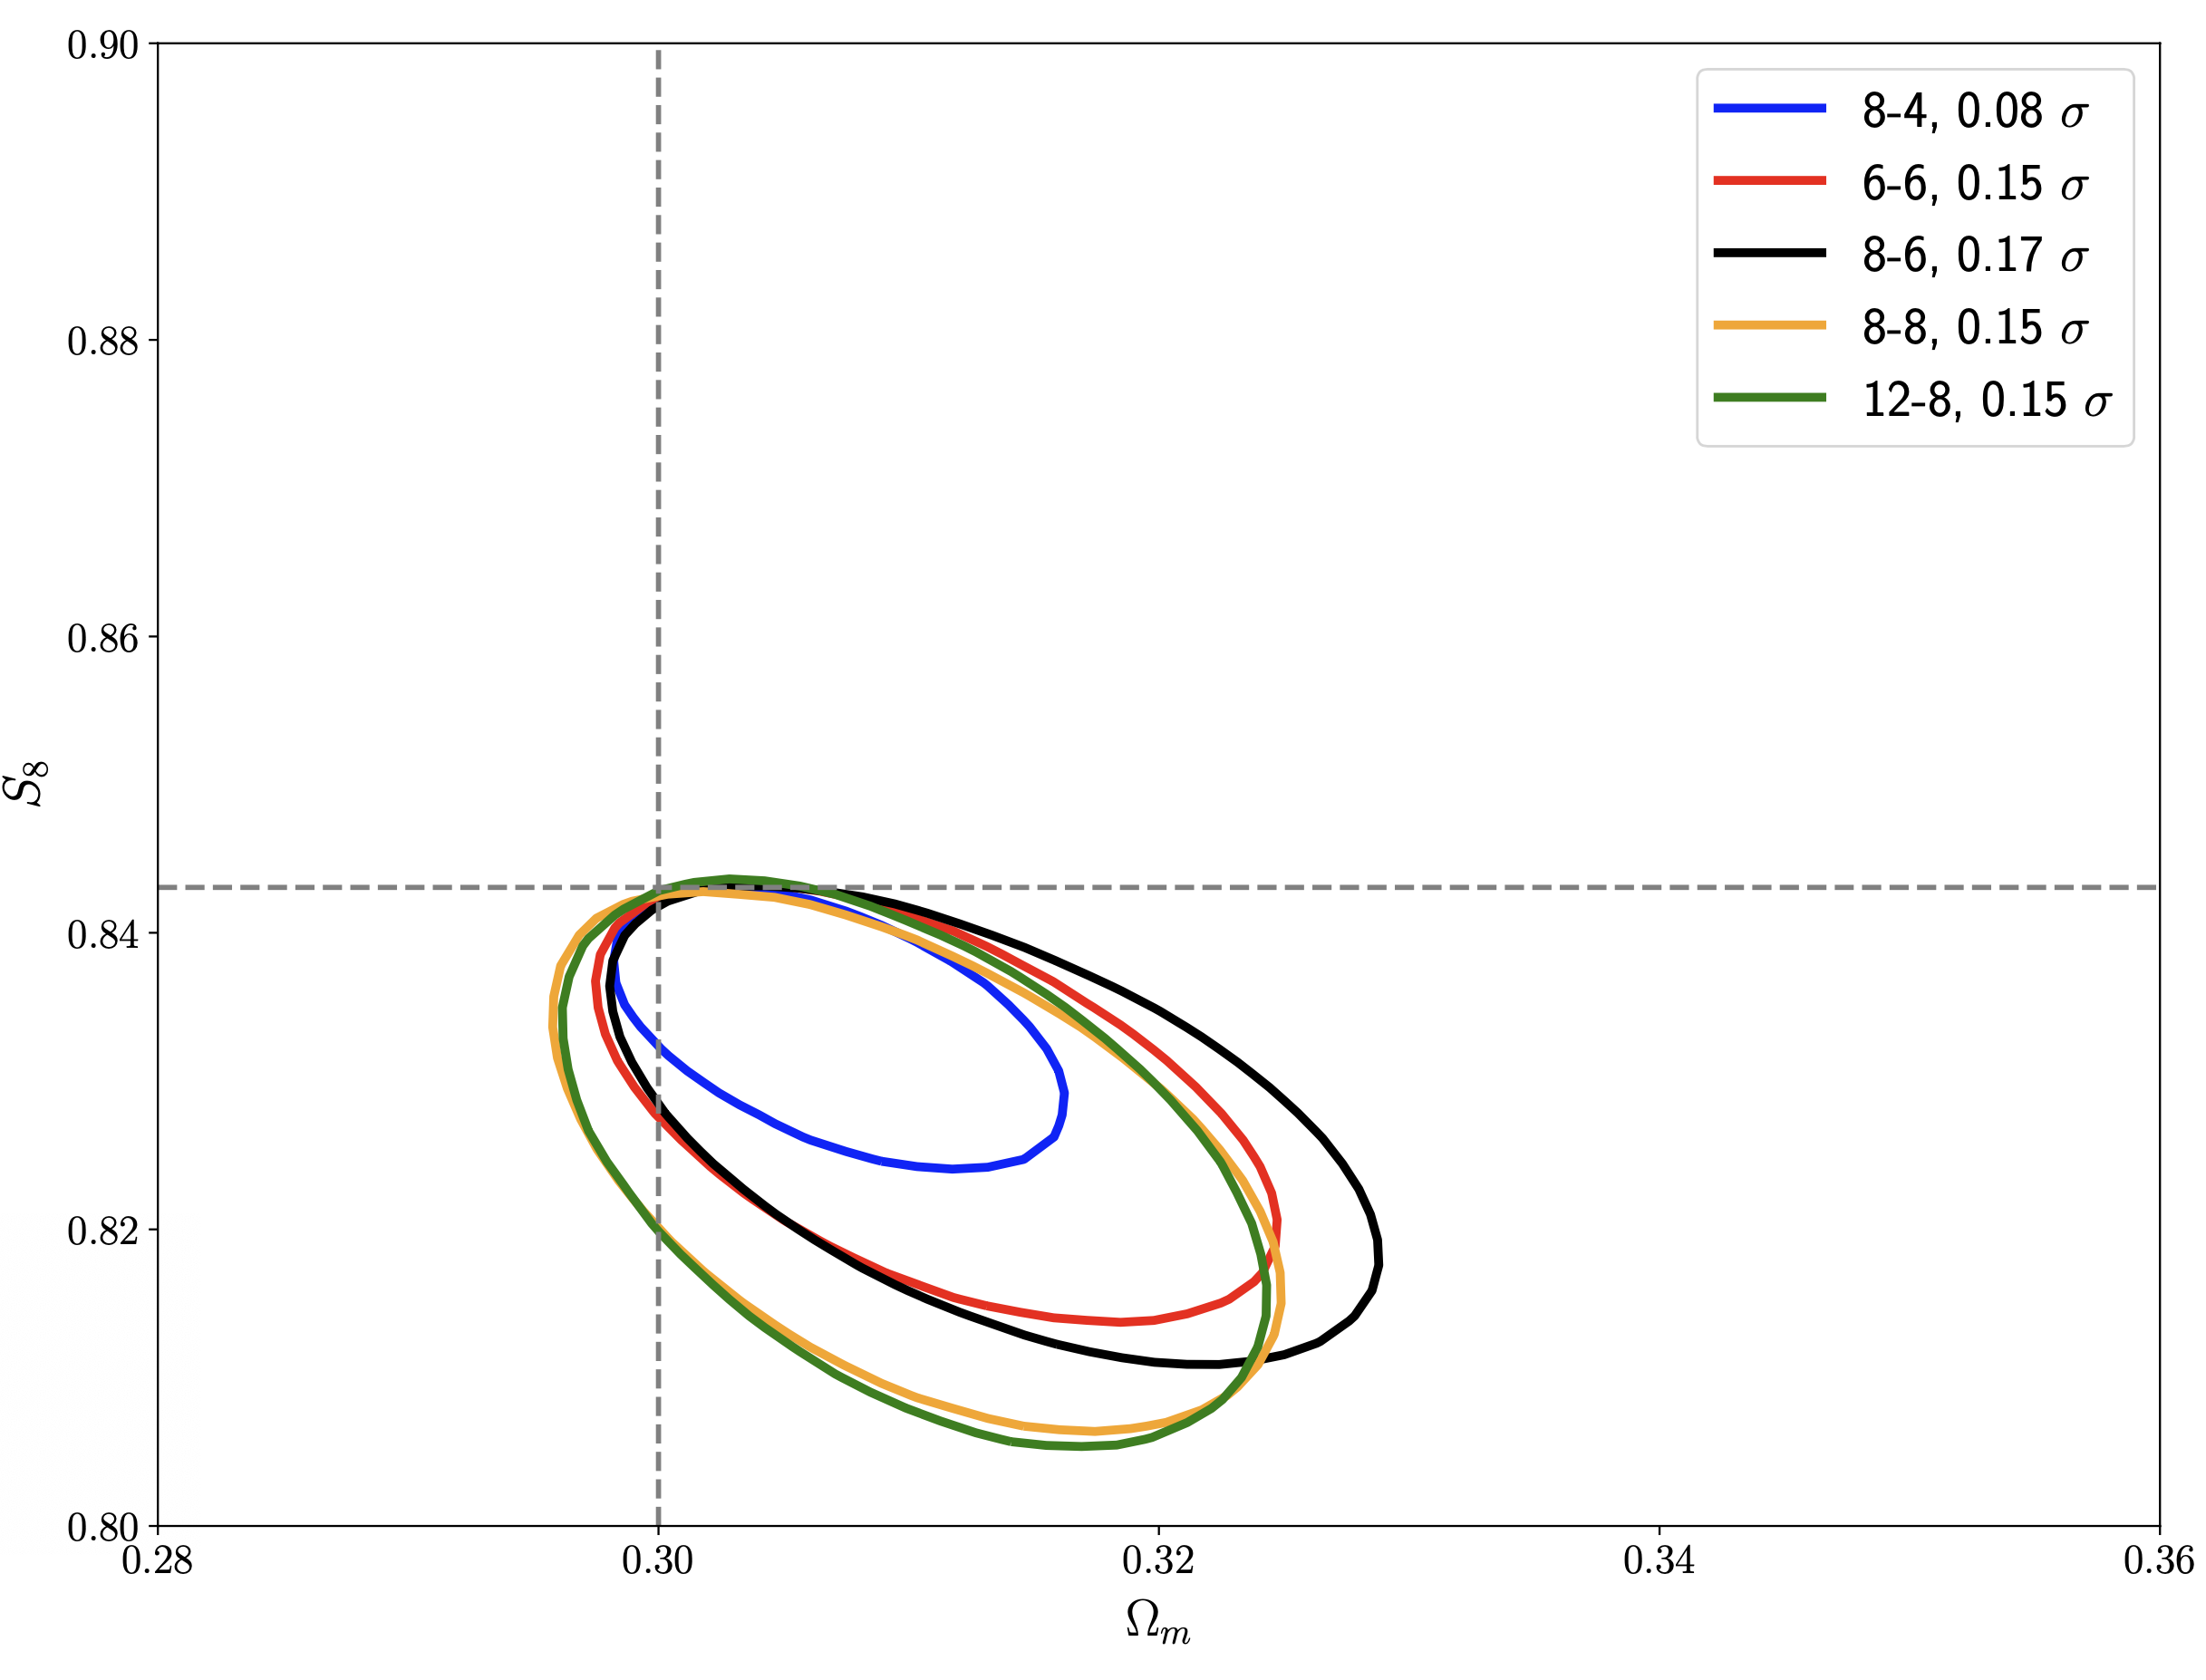
\includegraphics[width=0.5\textwidth,draft]{figs/temp.png}
% \caption[]{Show profile likelihood plots to show that we recover correct likelihood for cosmology parameters, while the posteriors are biased}
% \label{fig:prof_like}
% \end{figure}

% \begin{figure*}
% 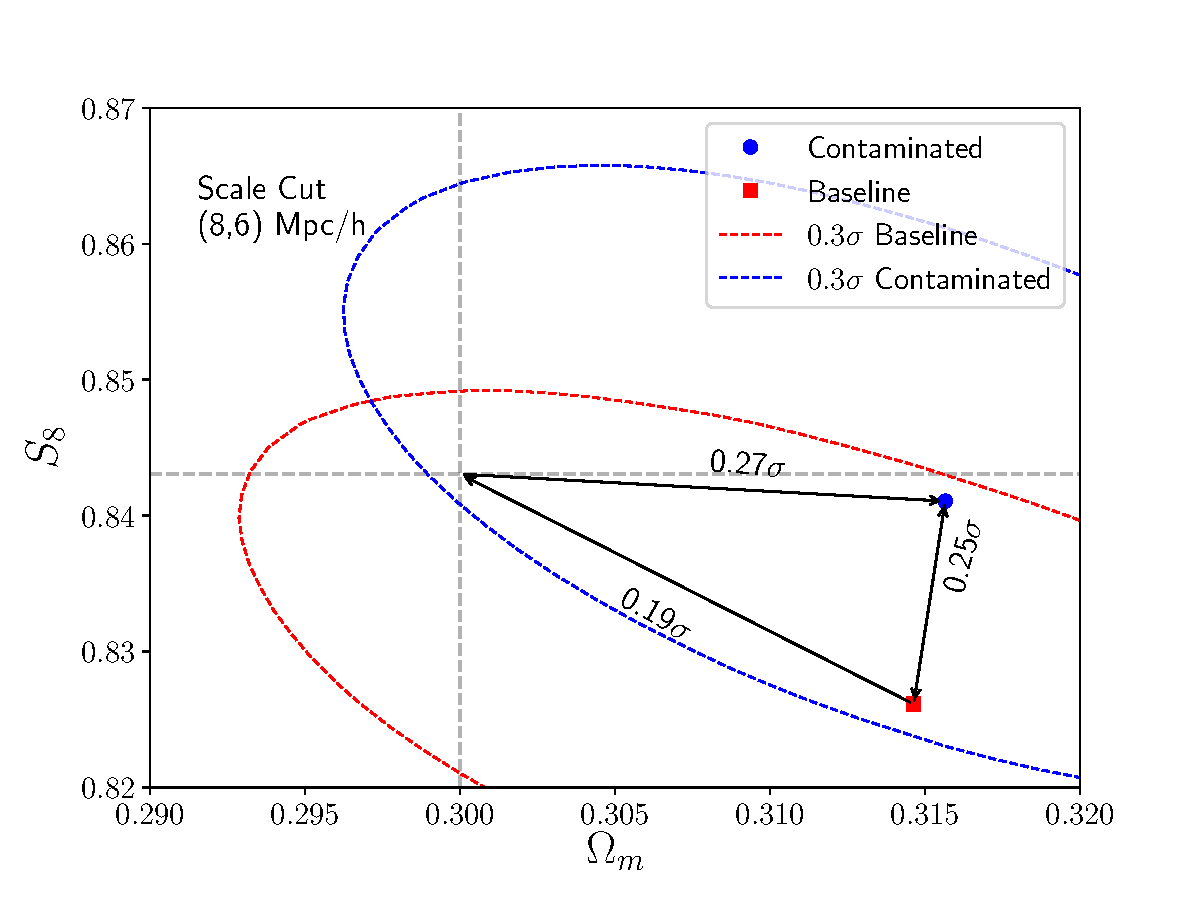
\includegraphics[width=\columnwidth]{figs/contour_2x2pt_sc_8_6.pdf}
% 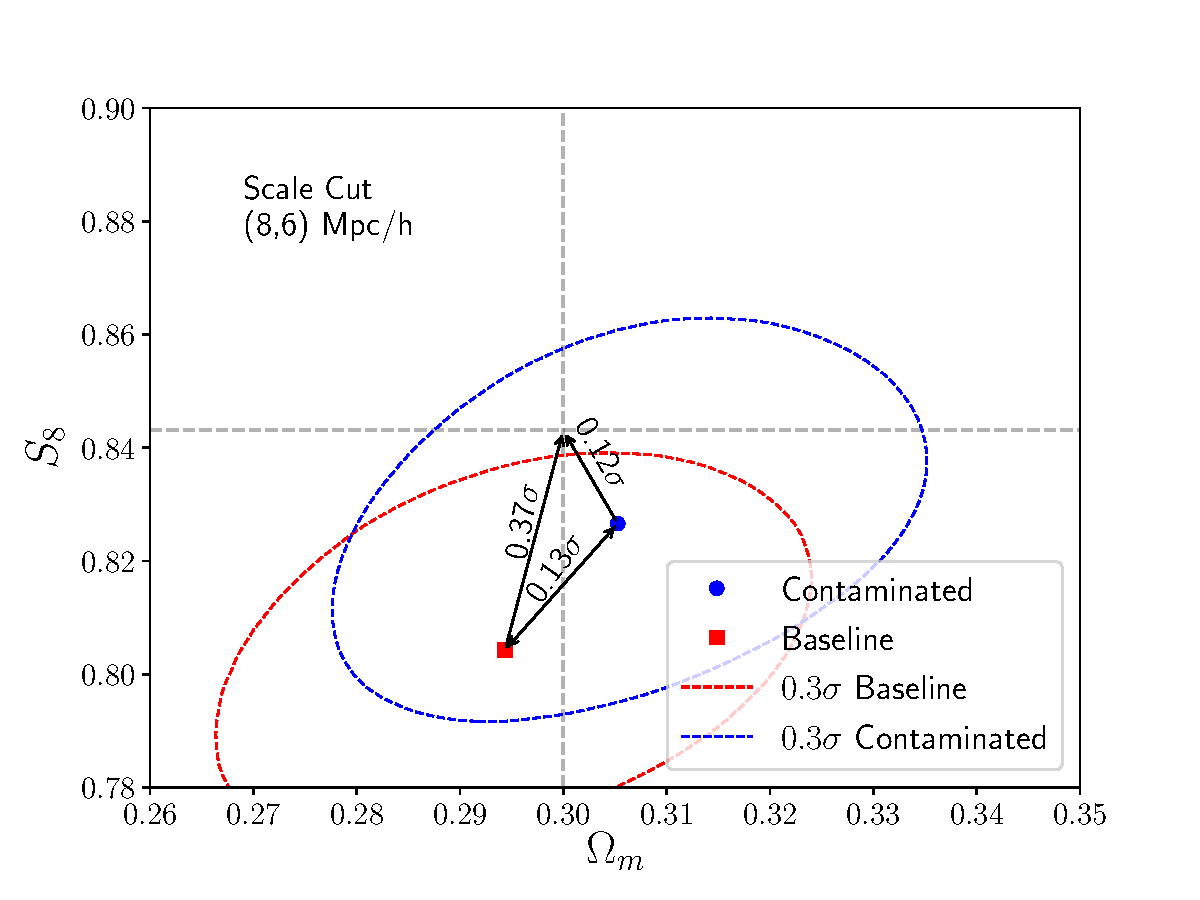
\includegraphics[width=\columnwidth]{figs/contour_2x2pt_sc_8_6_wcdm.pdf}
% \caption[]{Show the contour plots and biases in cosmology in the 2D space. Left is for $\Lambda$CDM and right is for $w$CDM. Show that the projection effects are much smaller in the 2D space}
% \label{fig:2d_simlike}
% \end{figure*}

% \begin{figure}
% 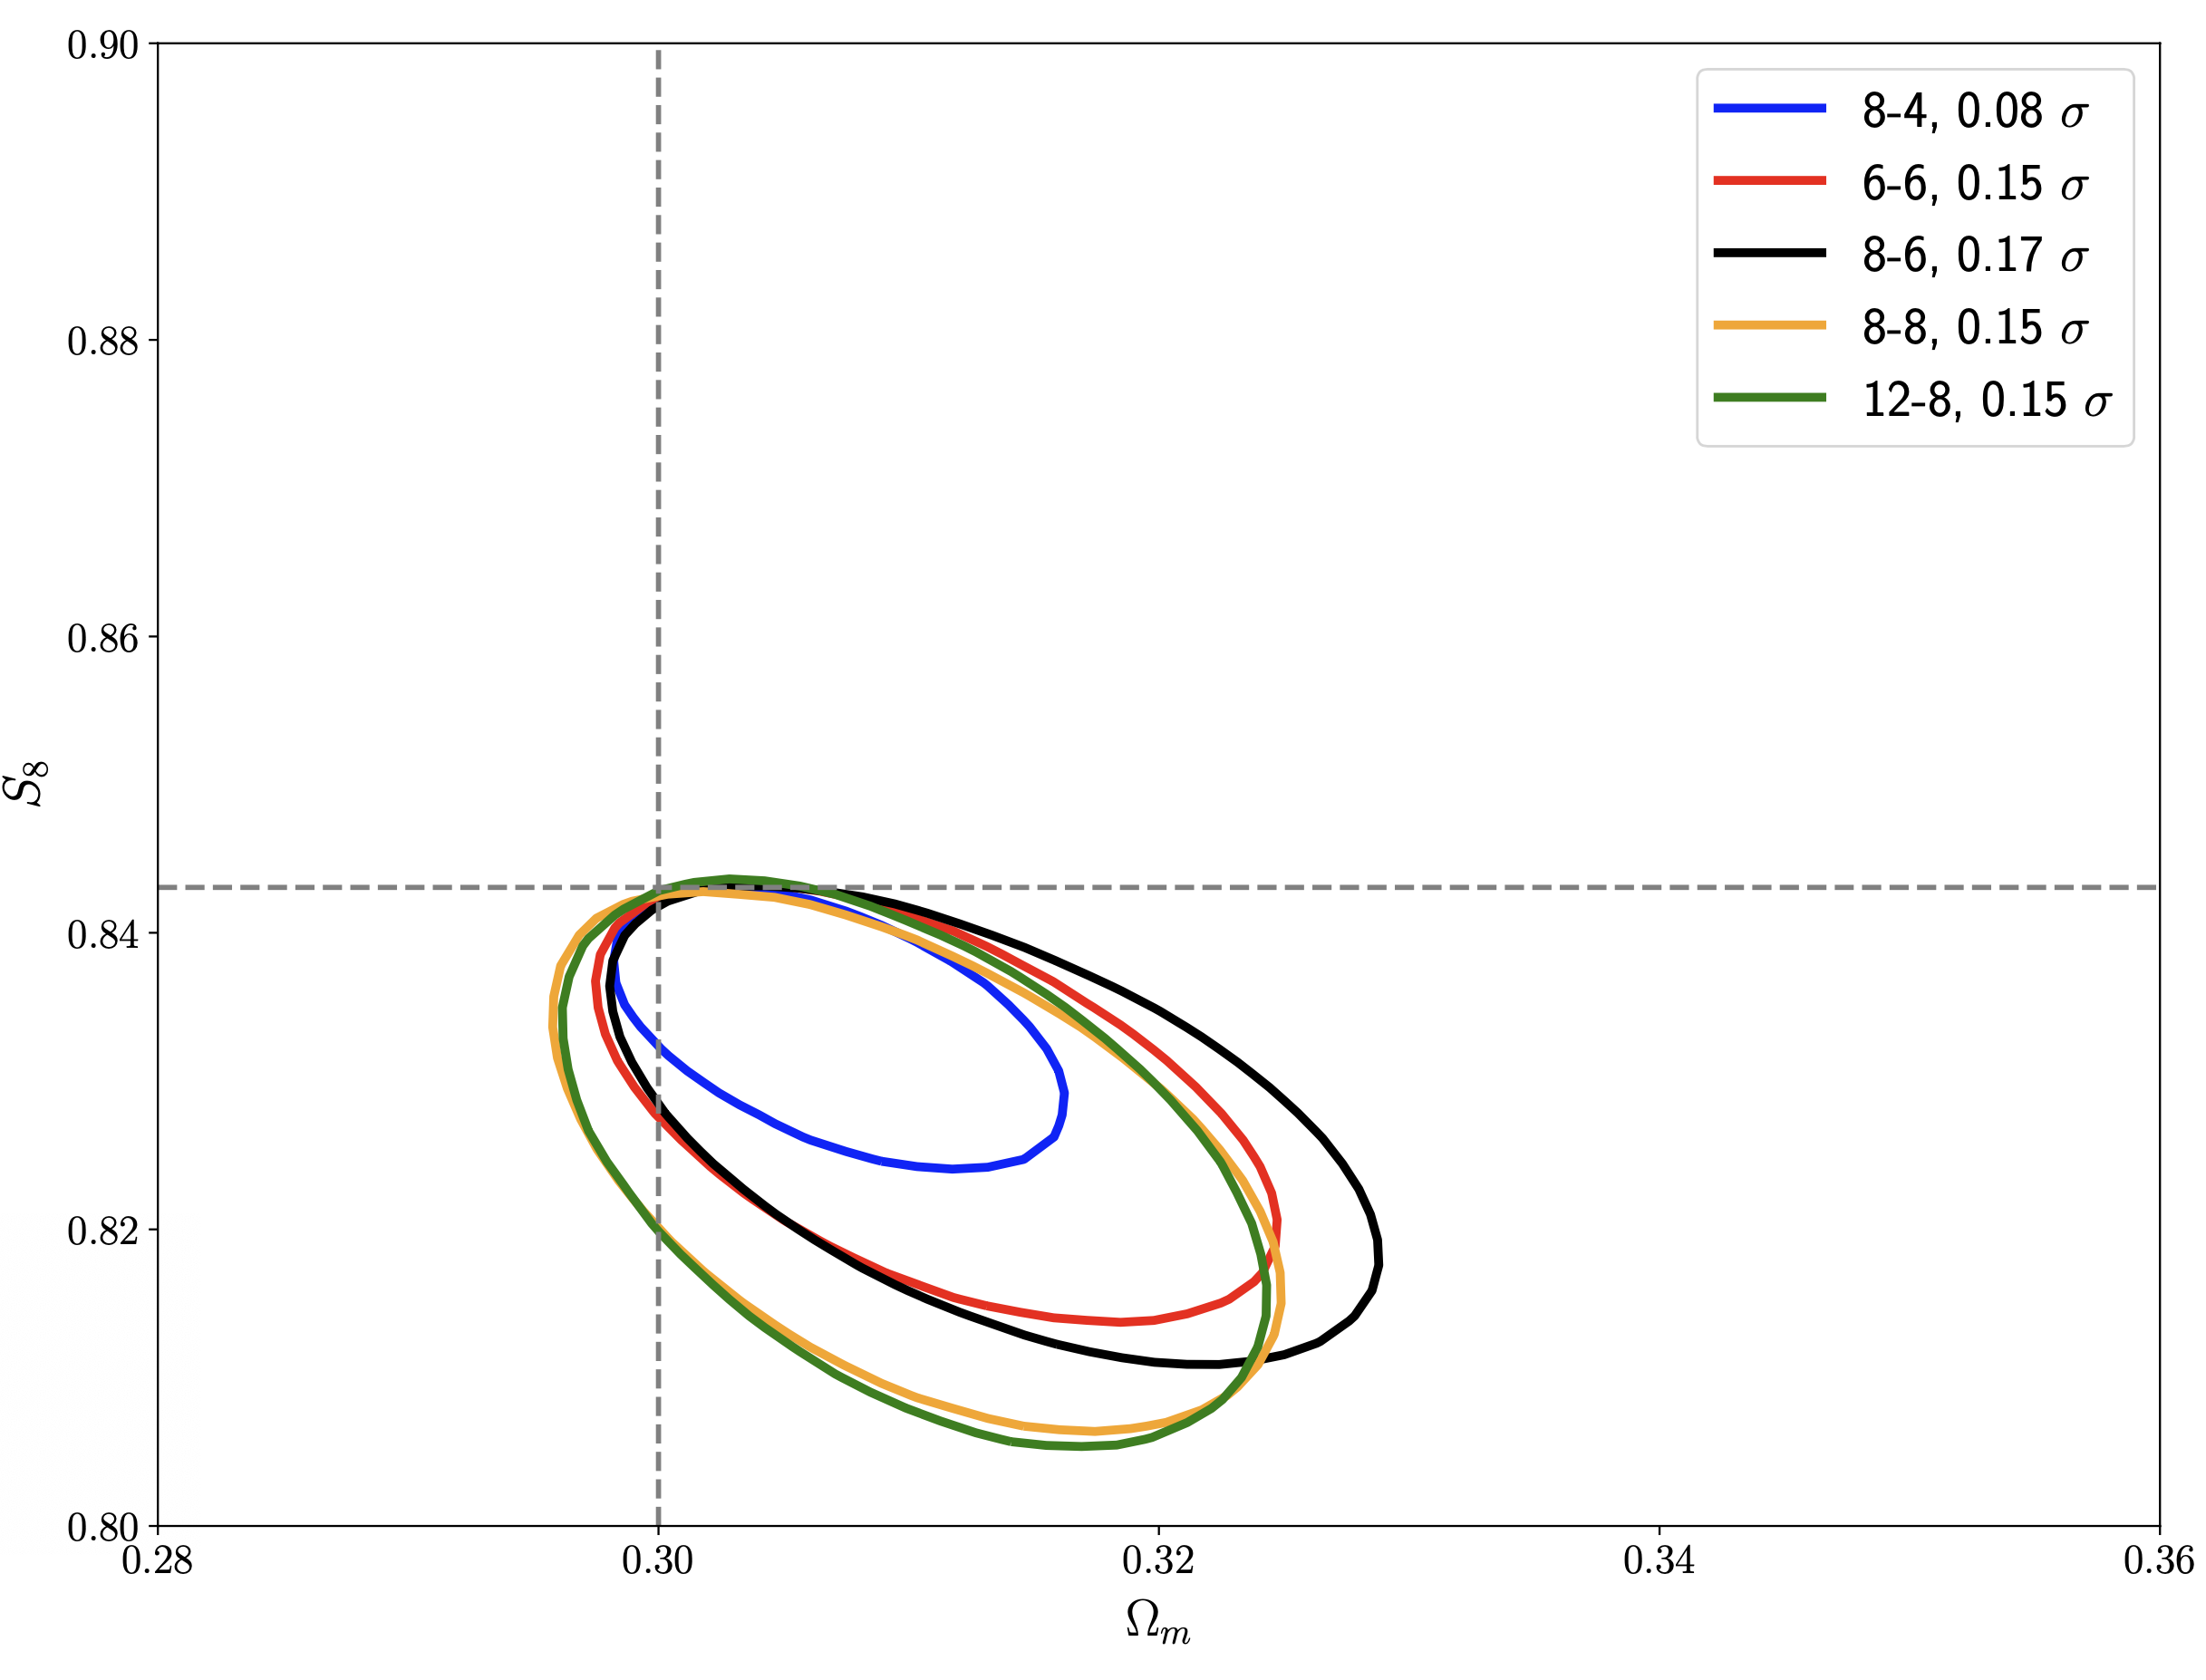
\includegraphics[width=0.5\textwidth,draft]{figs/temp.png}
% \caption[]{Show that the projection effects are smaller when using the prior set (ii), i.e. informative priors on $\theta_{\star}$, $\Omega_{\rm b} h^2$ and $n_s$.}
% \label{fig:simlike_cosmoprior}
% \end{figure}





%%%%%%%%%%%%%%%%%%%%%%%%%%%%%%%%%%%%%%%%%%%%%%%%%%


% Don't change these lines
\bsp	% typesetting comment
\label{lastpage}

% \bibliographystyle{apsrev4-1}
% \bibliography{ref} 

\end{document}

% End of mnras_template.tex